\begin{figure*}[!tp]
\centering
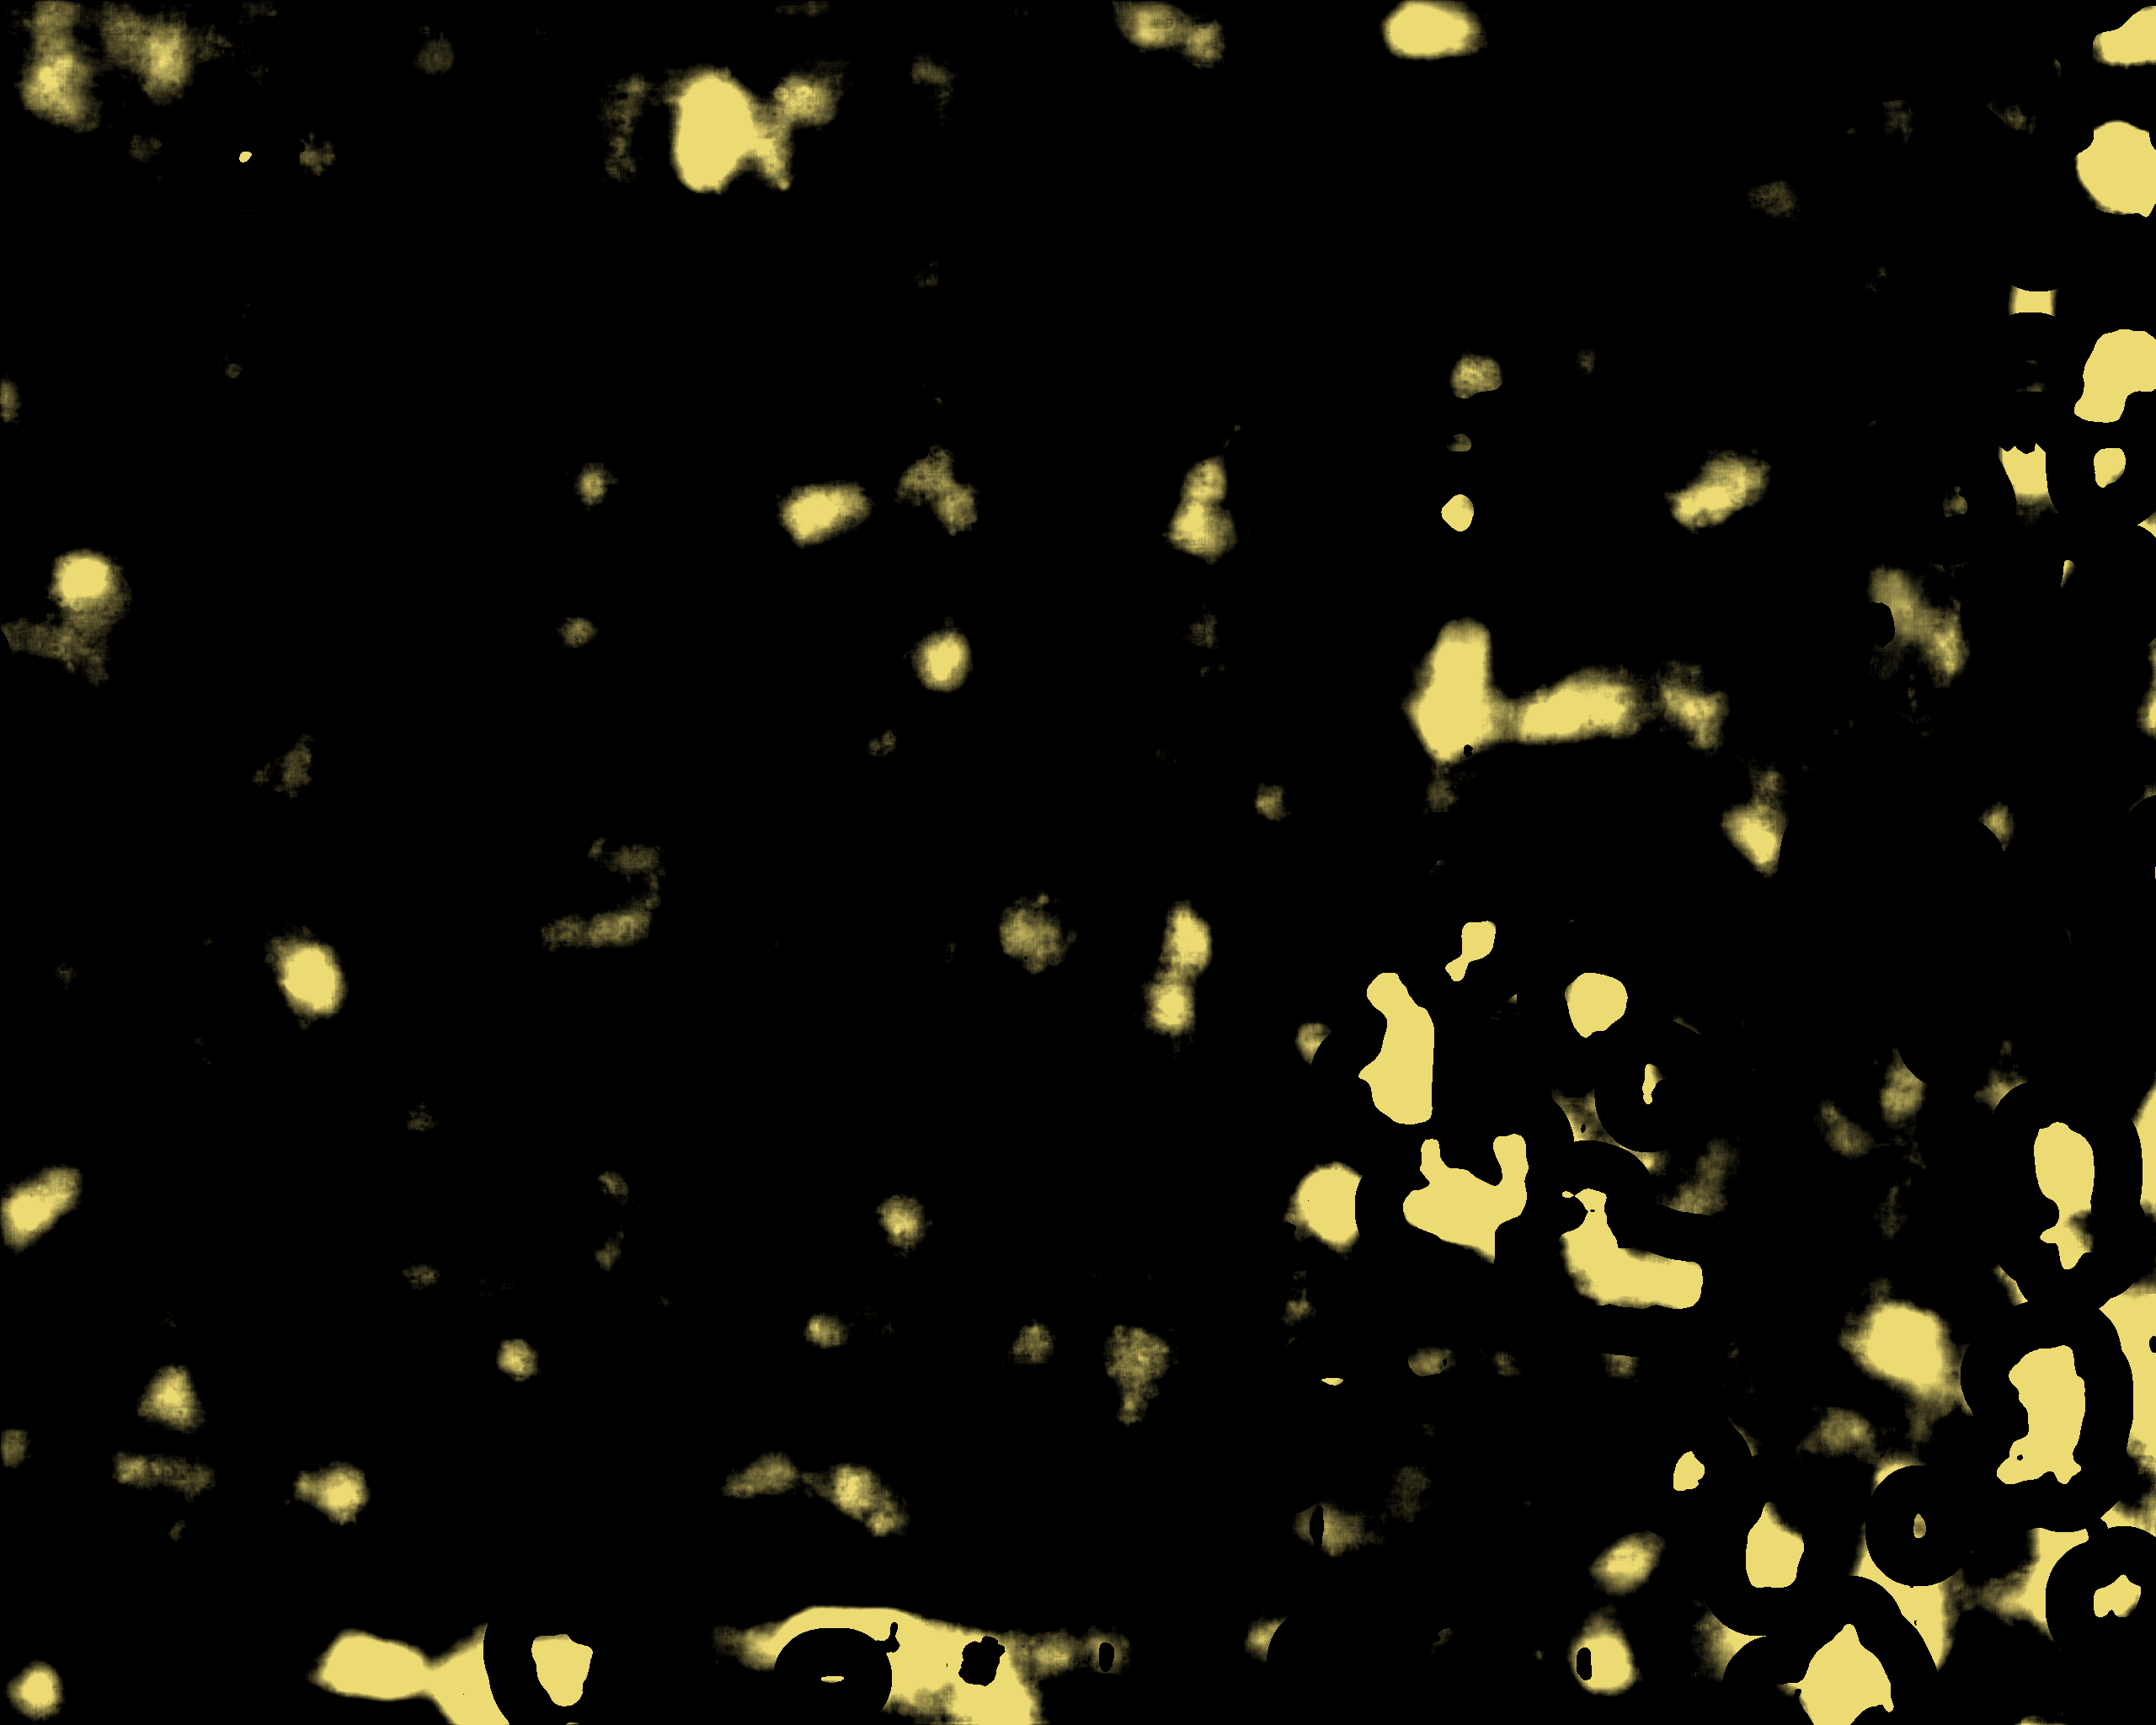
\includegraphics[width=0.29\textwidth]{../figures/m3/20250510172639_1_reader-v3.png}
\hspace{3pt}
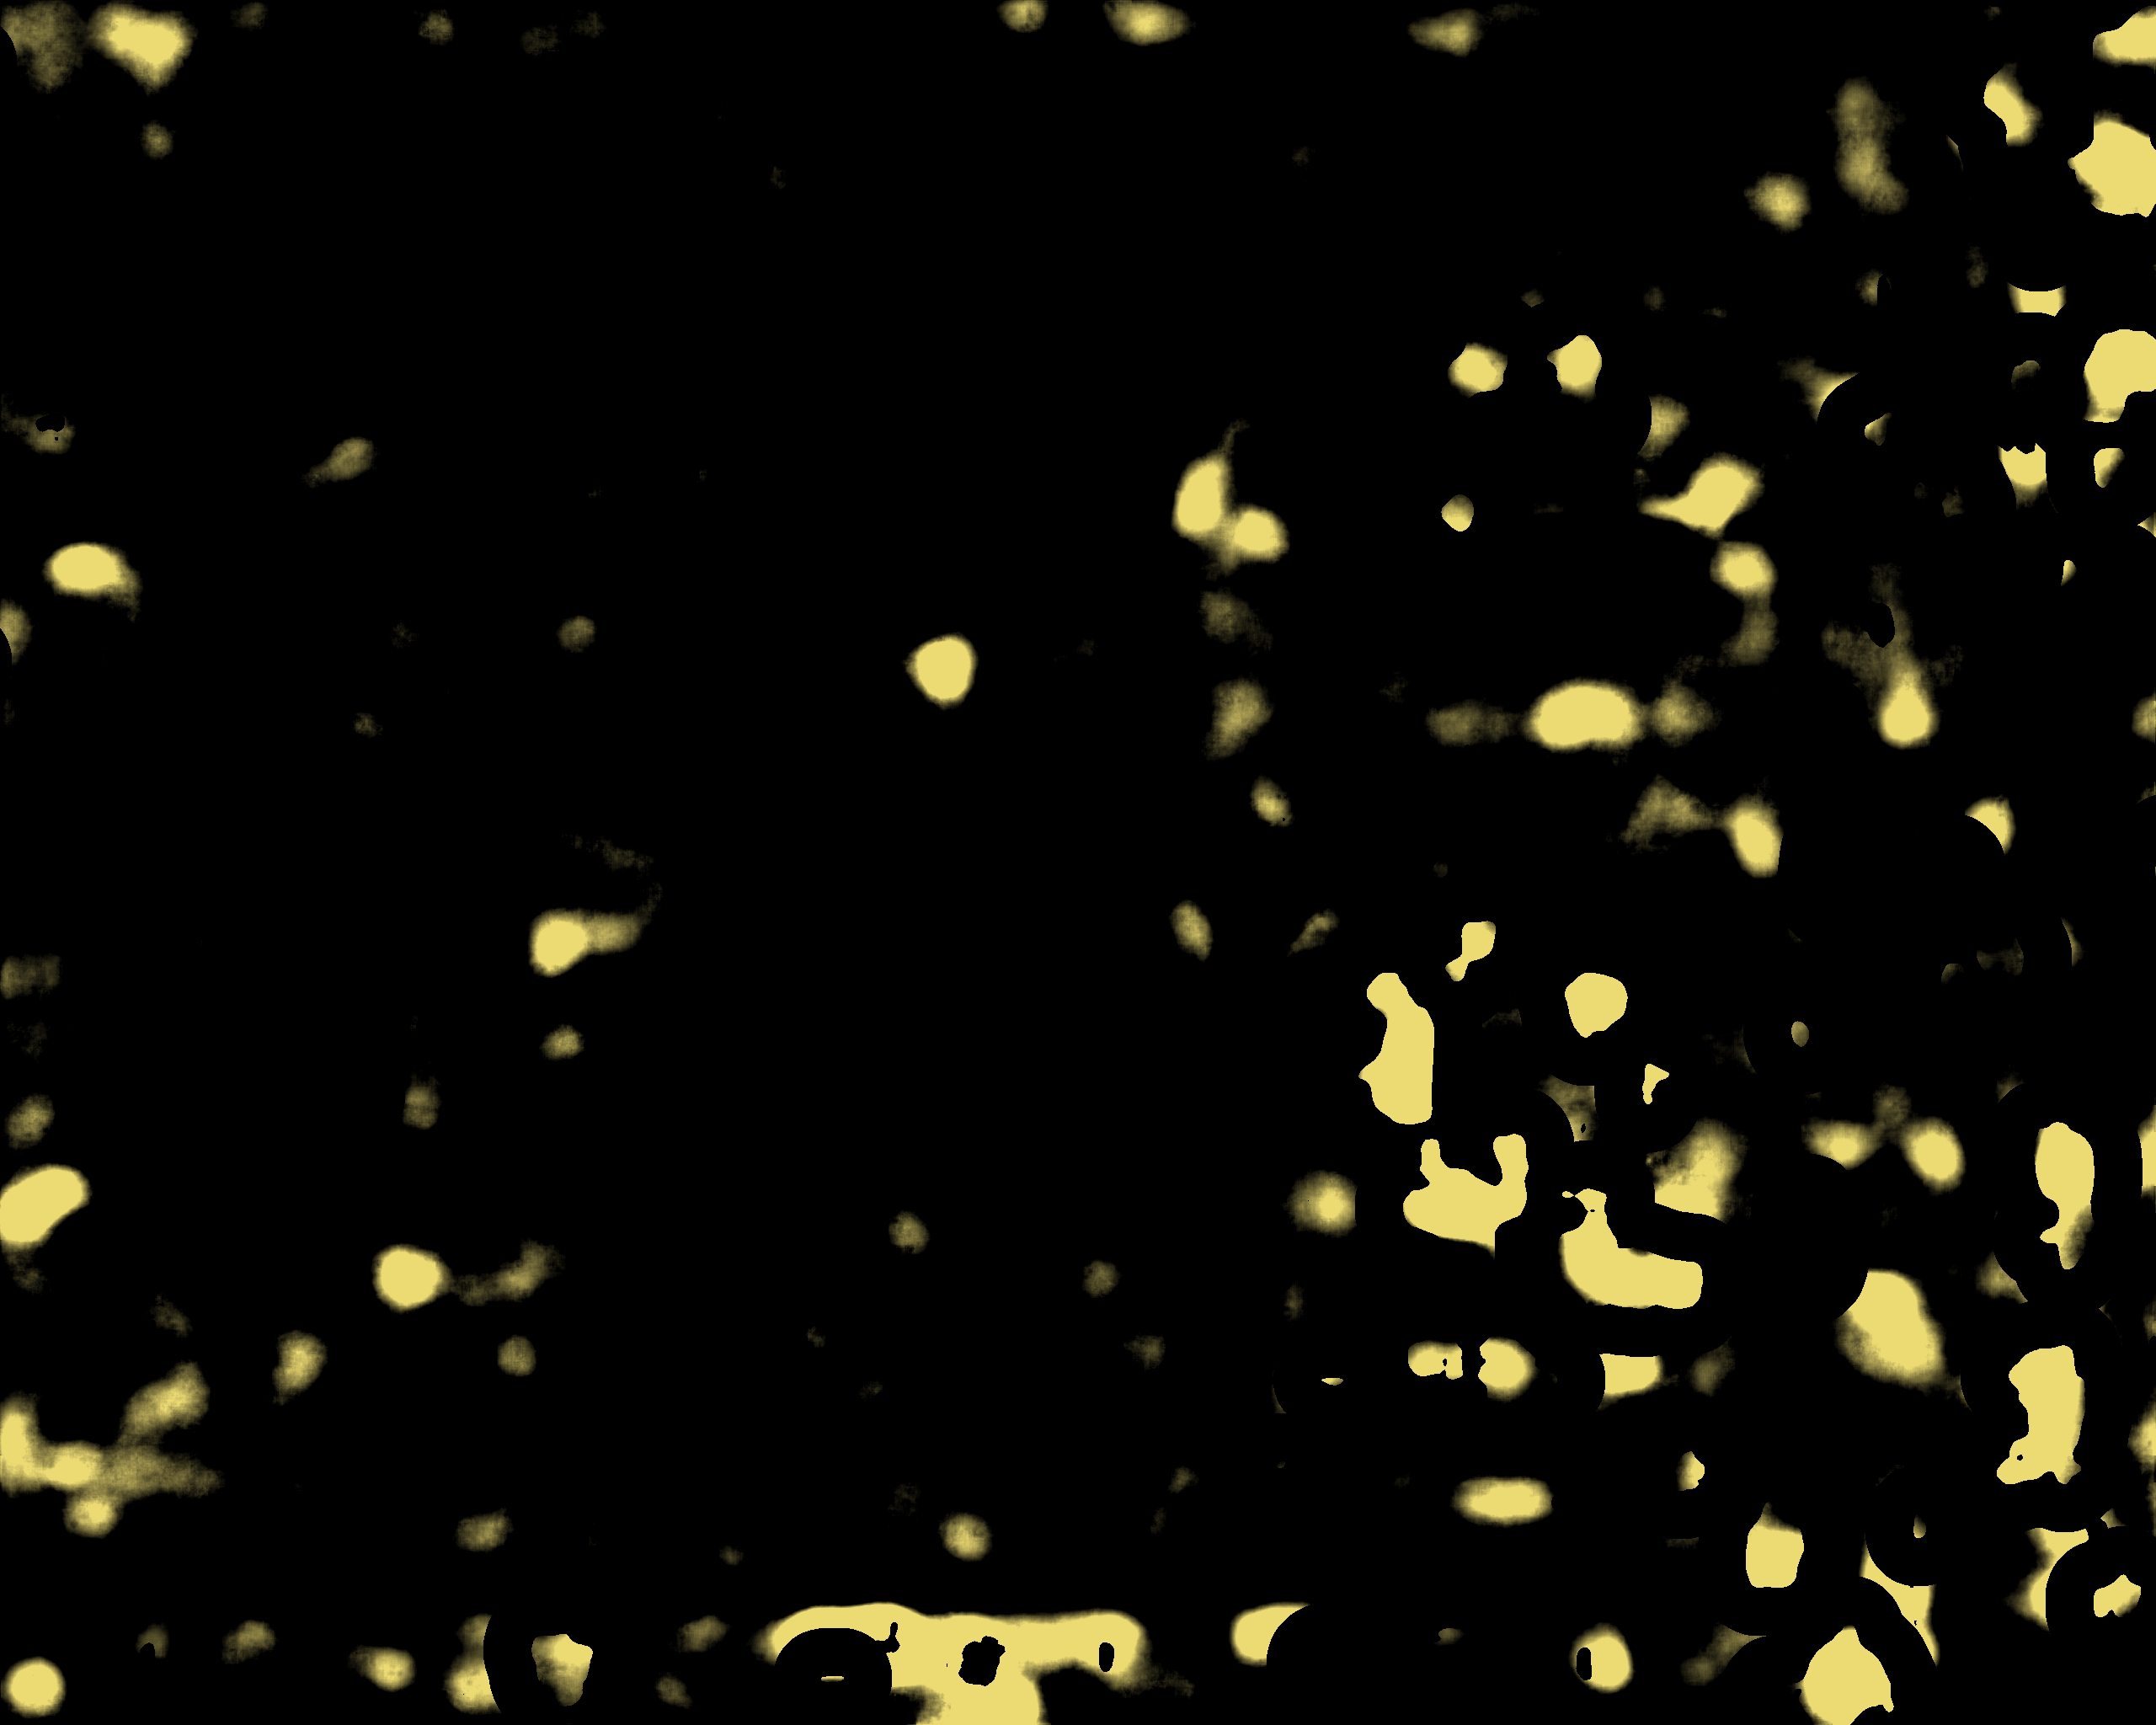
\includegraphics[width=0.29\textwidth]{../figures/m3/20250510172639_2_m3.png}
\hspace{3pt}
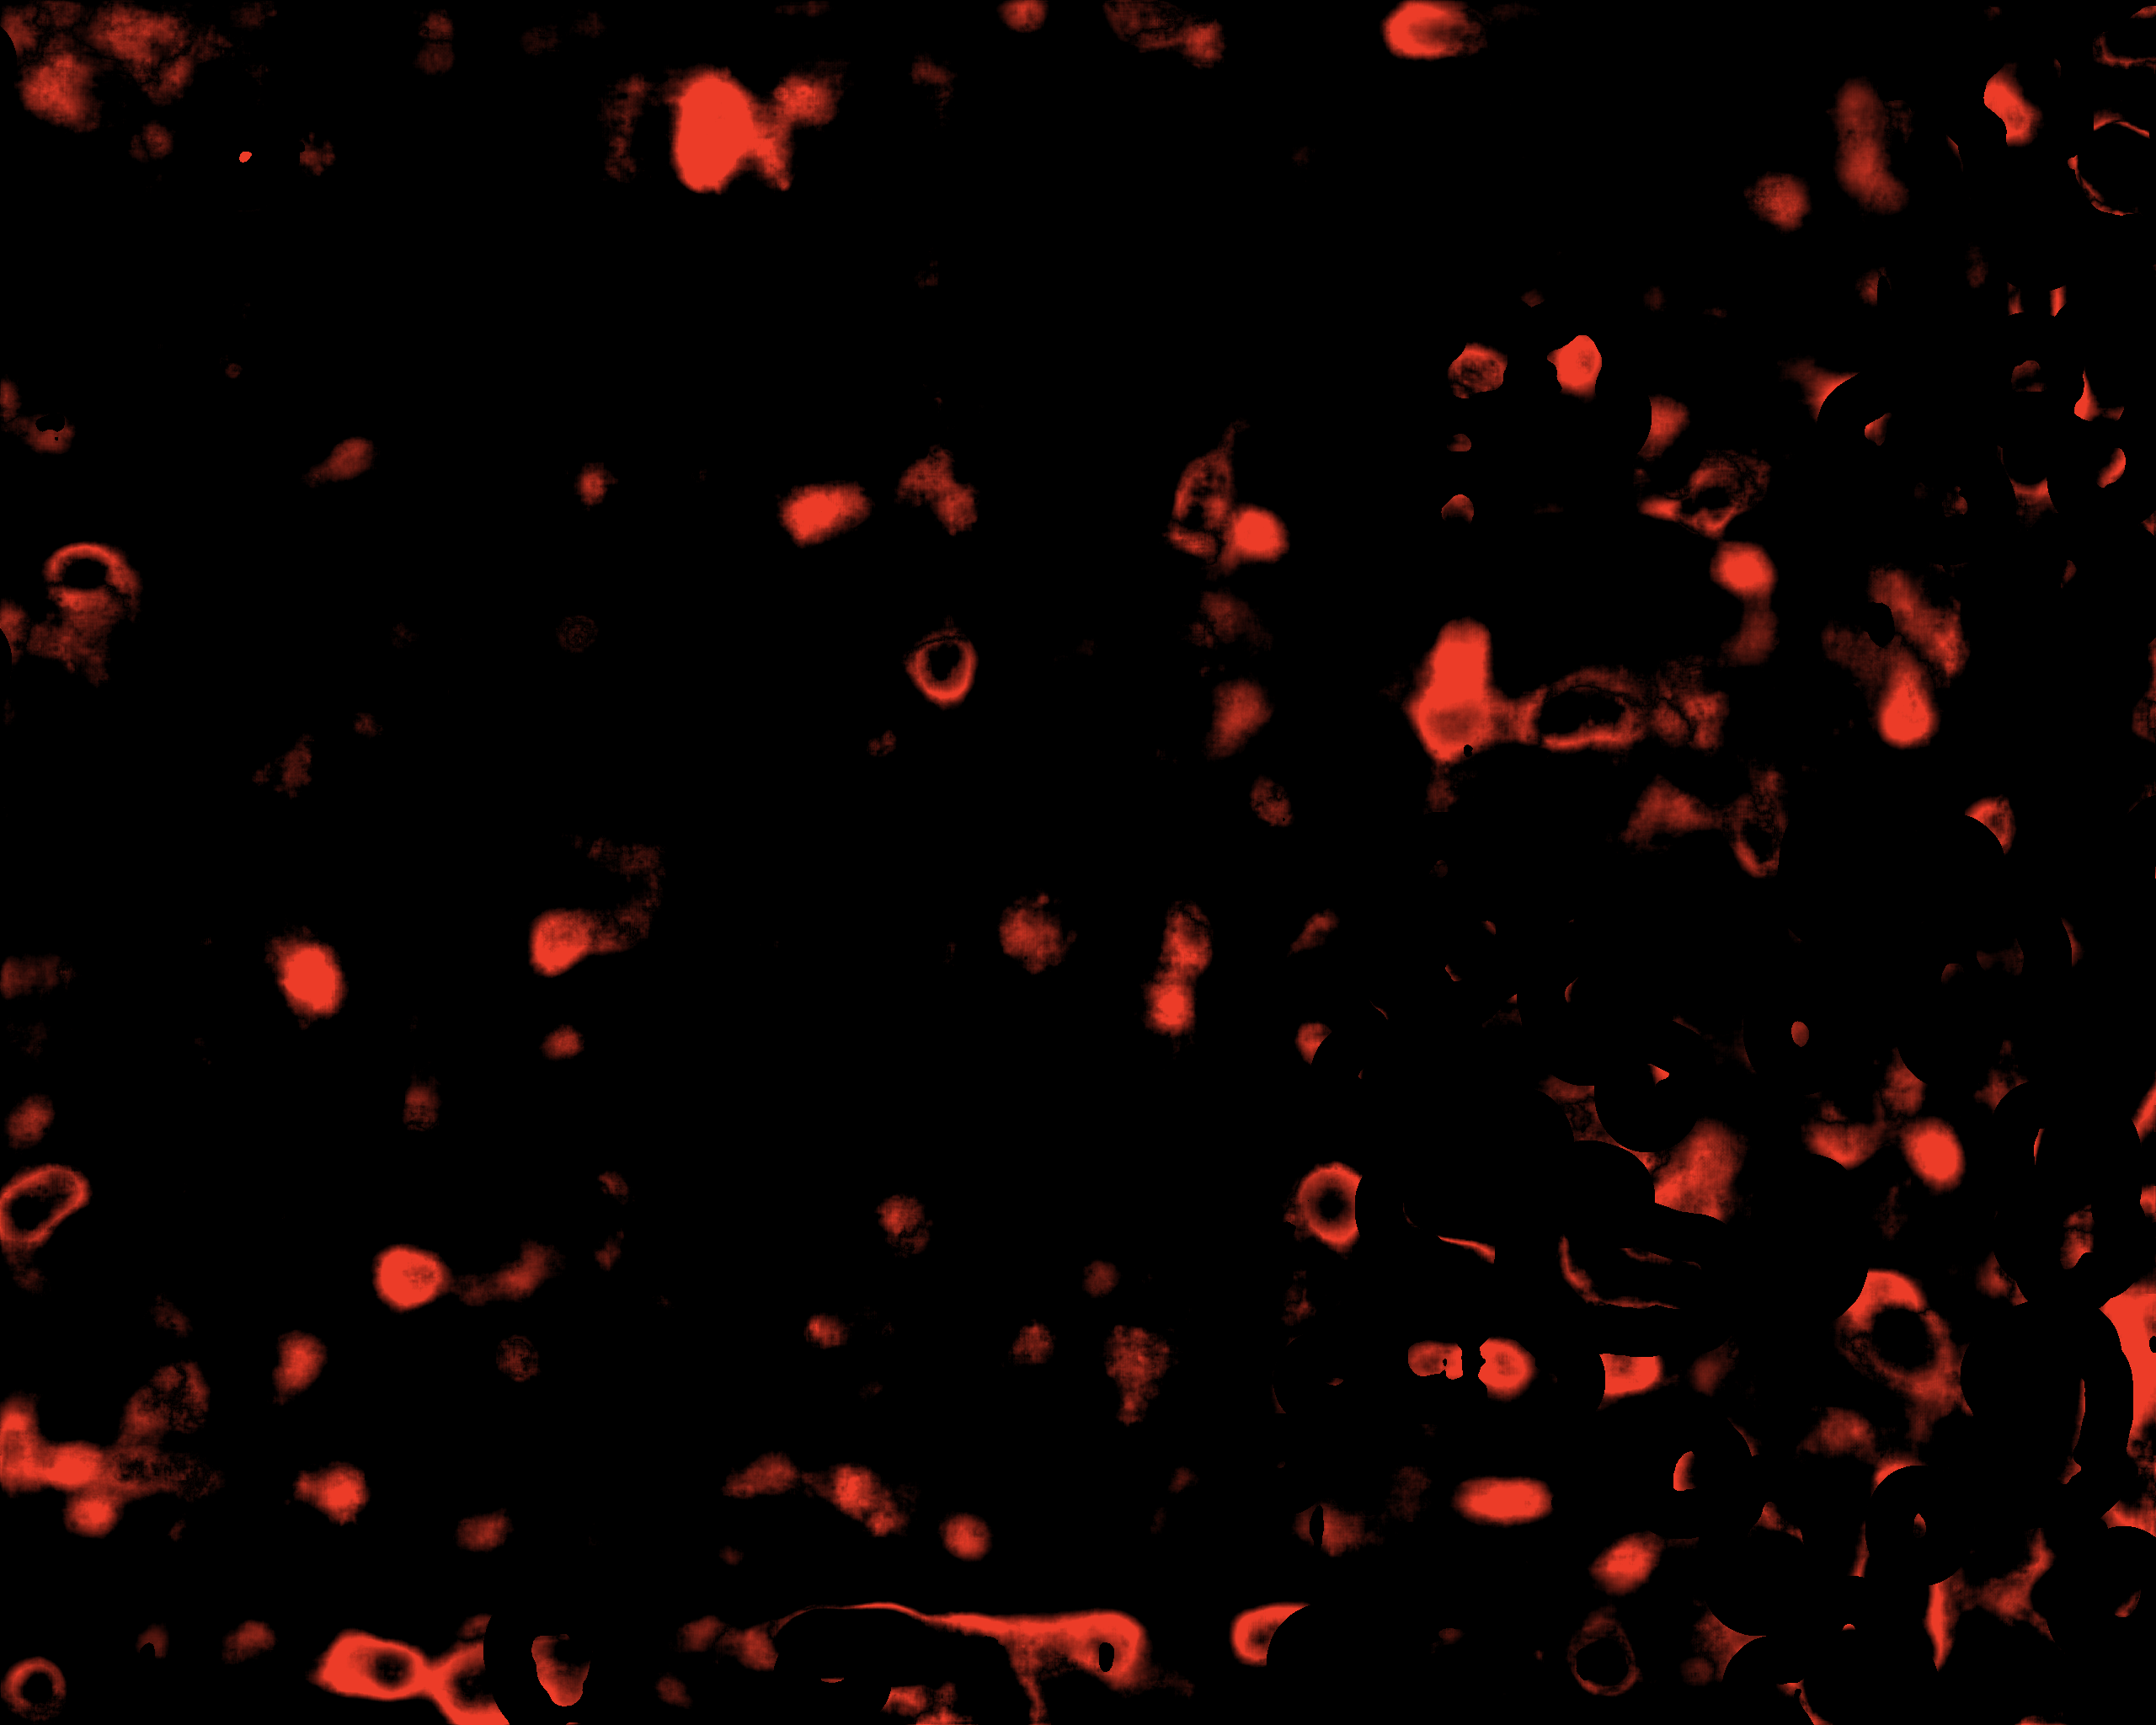
\includegraphics[width=0.29\textwidth]{../figures/m3/20250510172639_3_difference.png}
\caption{Held-out unit 0009B$\cdot$172639. Left, Reader v3 (AUC 0.8456); centre, \MtName{} (AUC 0.8909); right, the red difference between the two maps. Each map is stretched between its own percentiles, the panels are shown at the full resolution of the file.}\label{fig:m3-20250510172639}
\end{figure*}

\begin{figure*}[!tp]
\centering
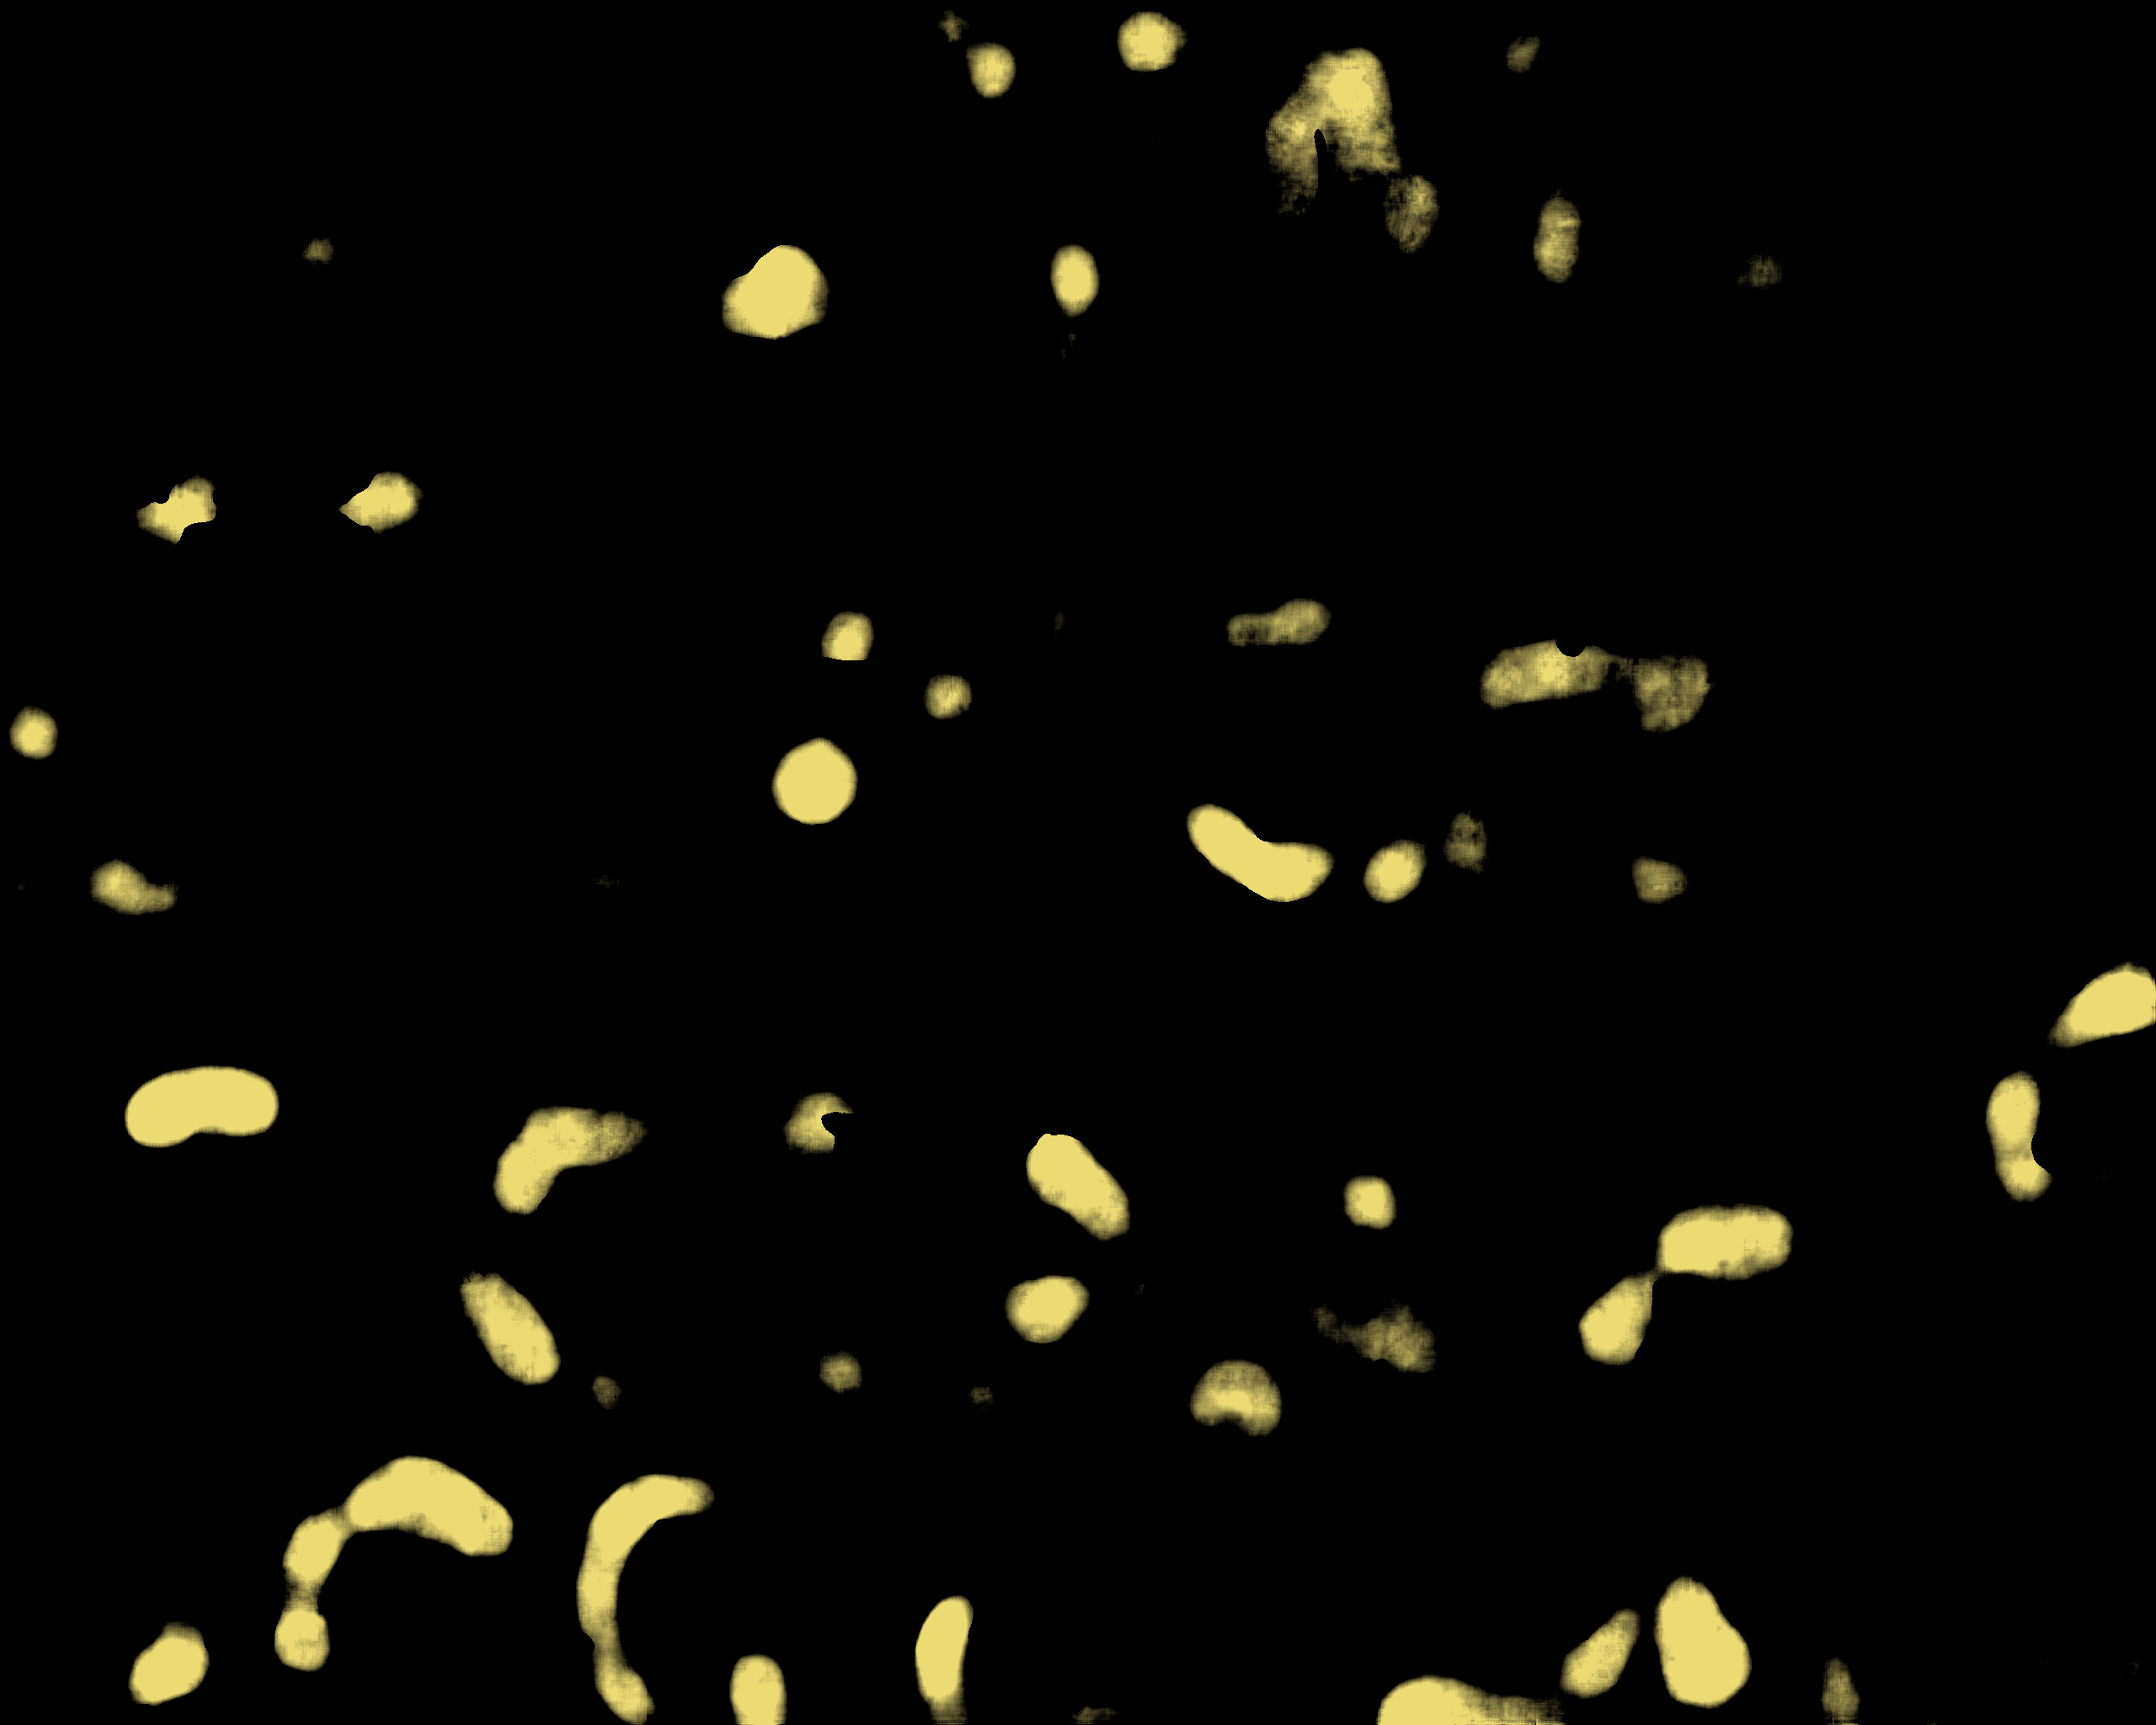
\includegraphics[width=0.29\textwidth]{../figures/m3/20250919125754_1_reader-v3.png}
\hspace{3pt}
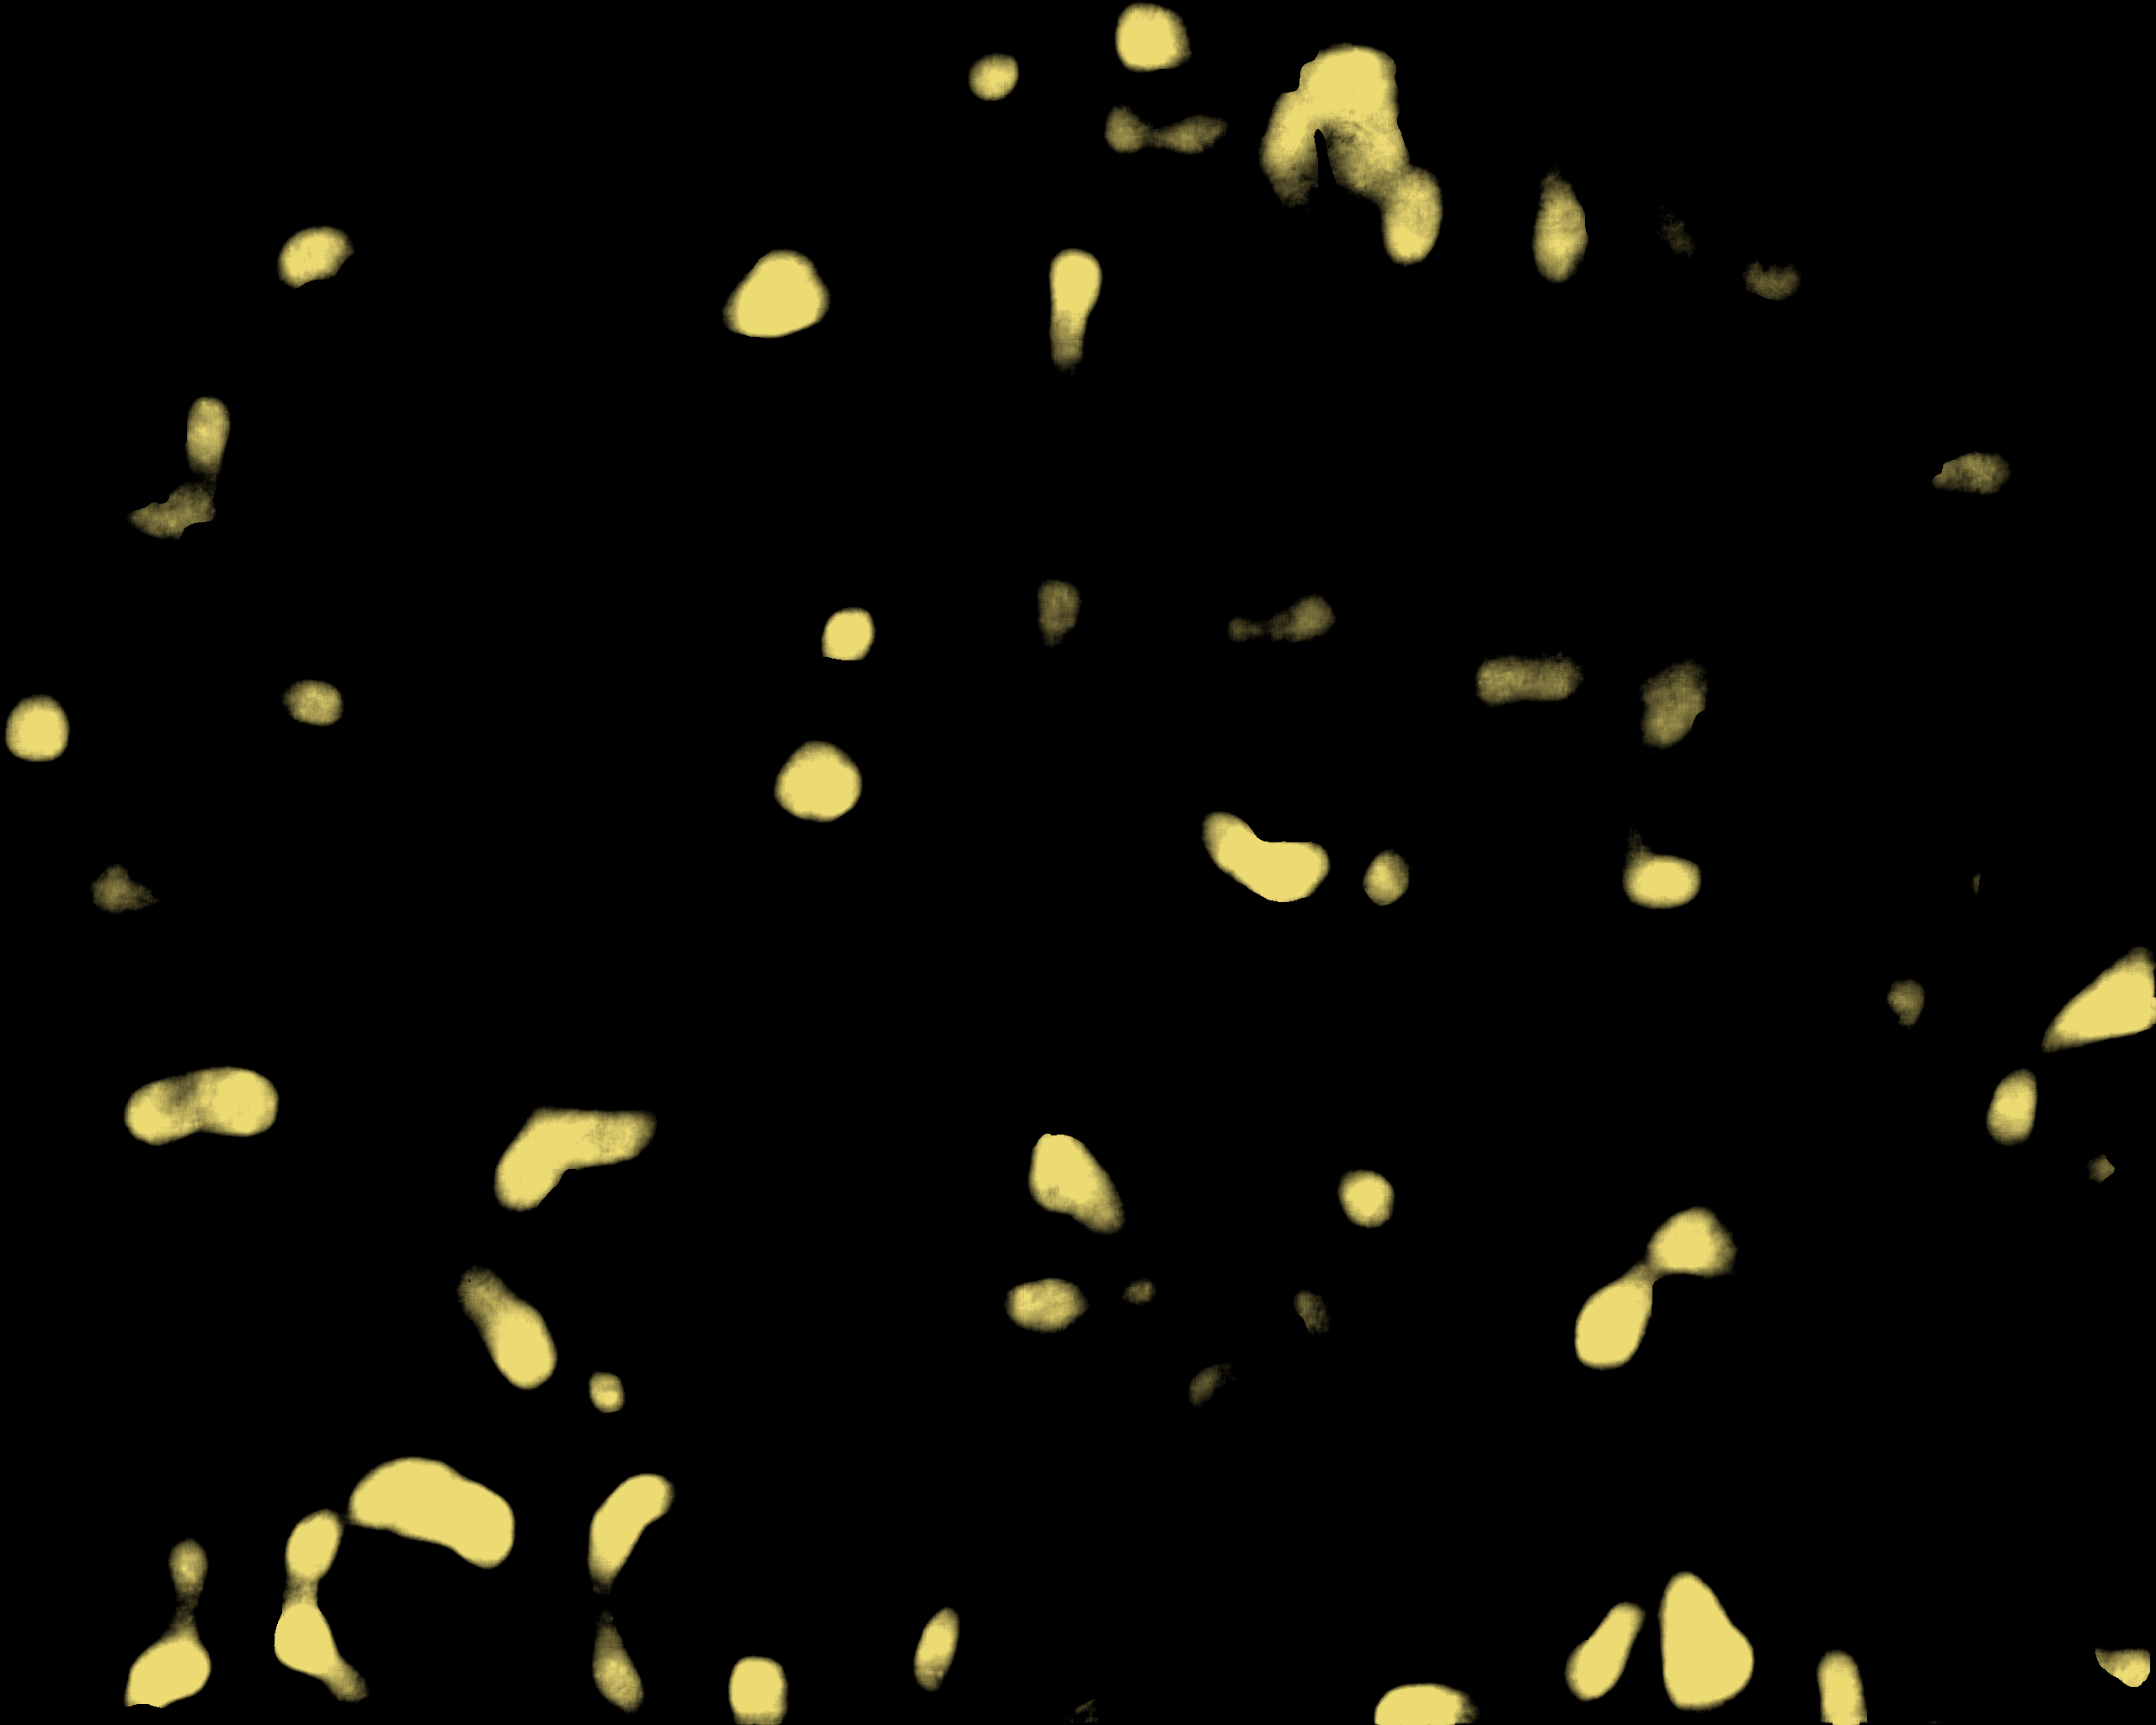
\includegraphics[width=0.29\textwidth]{../figures/m3/20250919125754_2_m3.png}
\hspace{3pt}
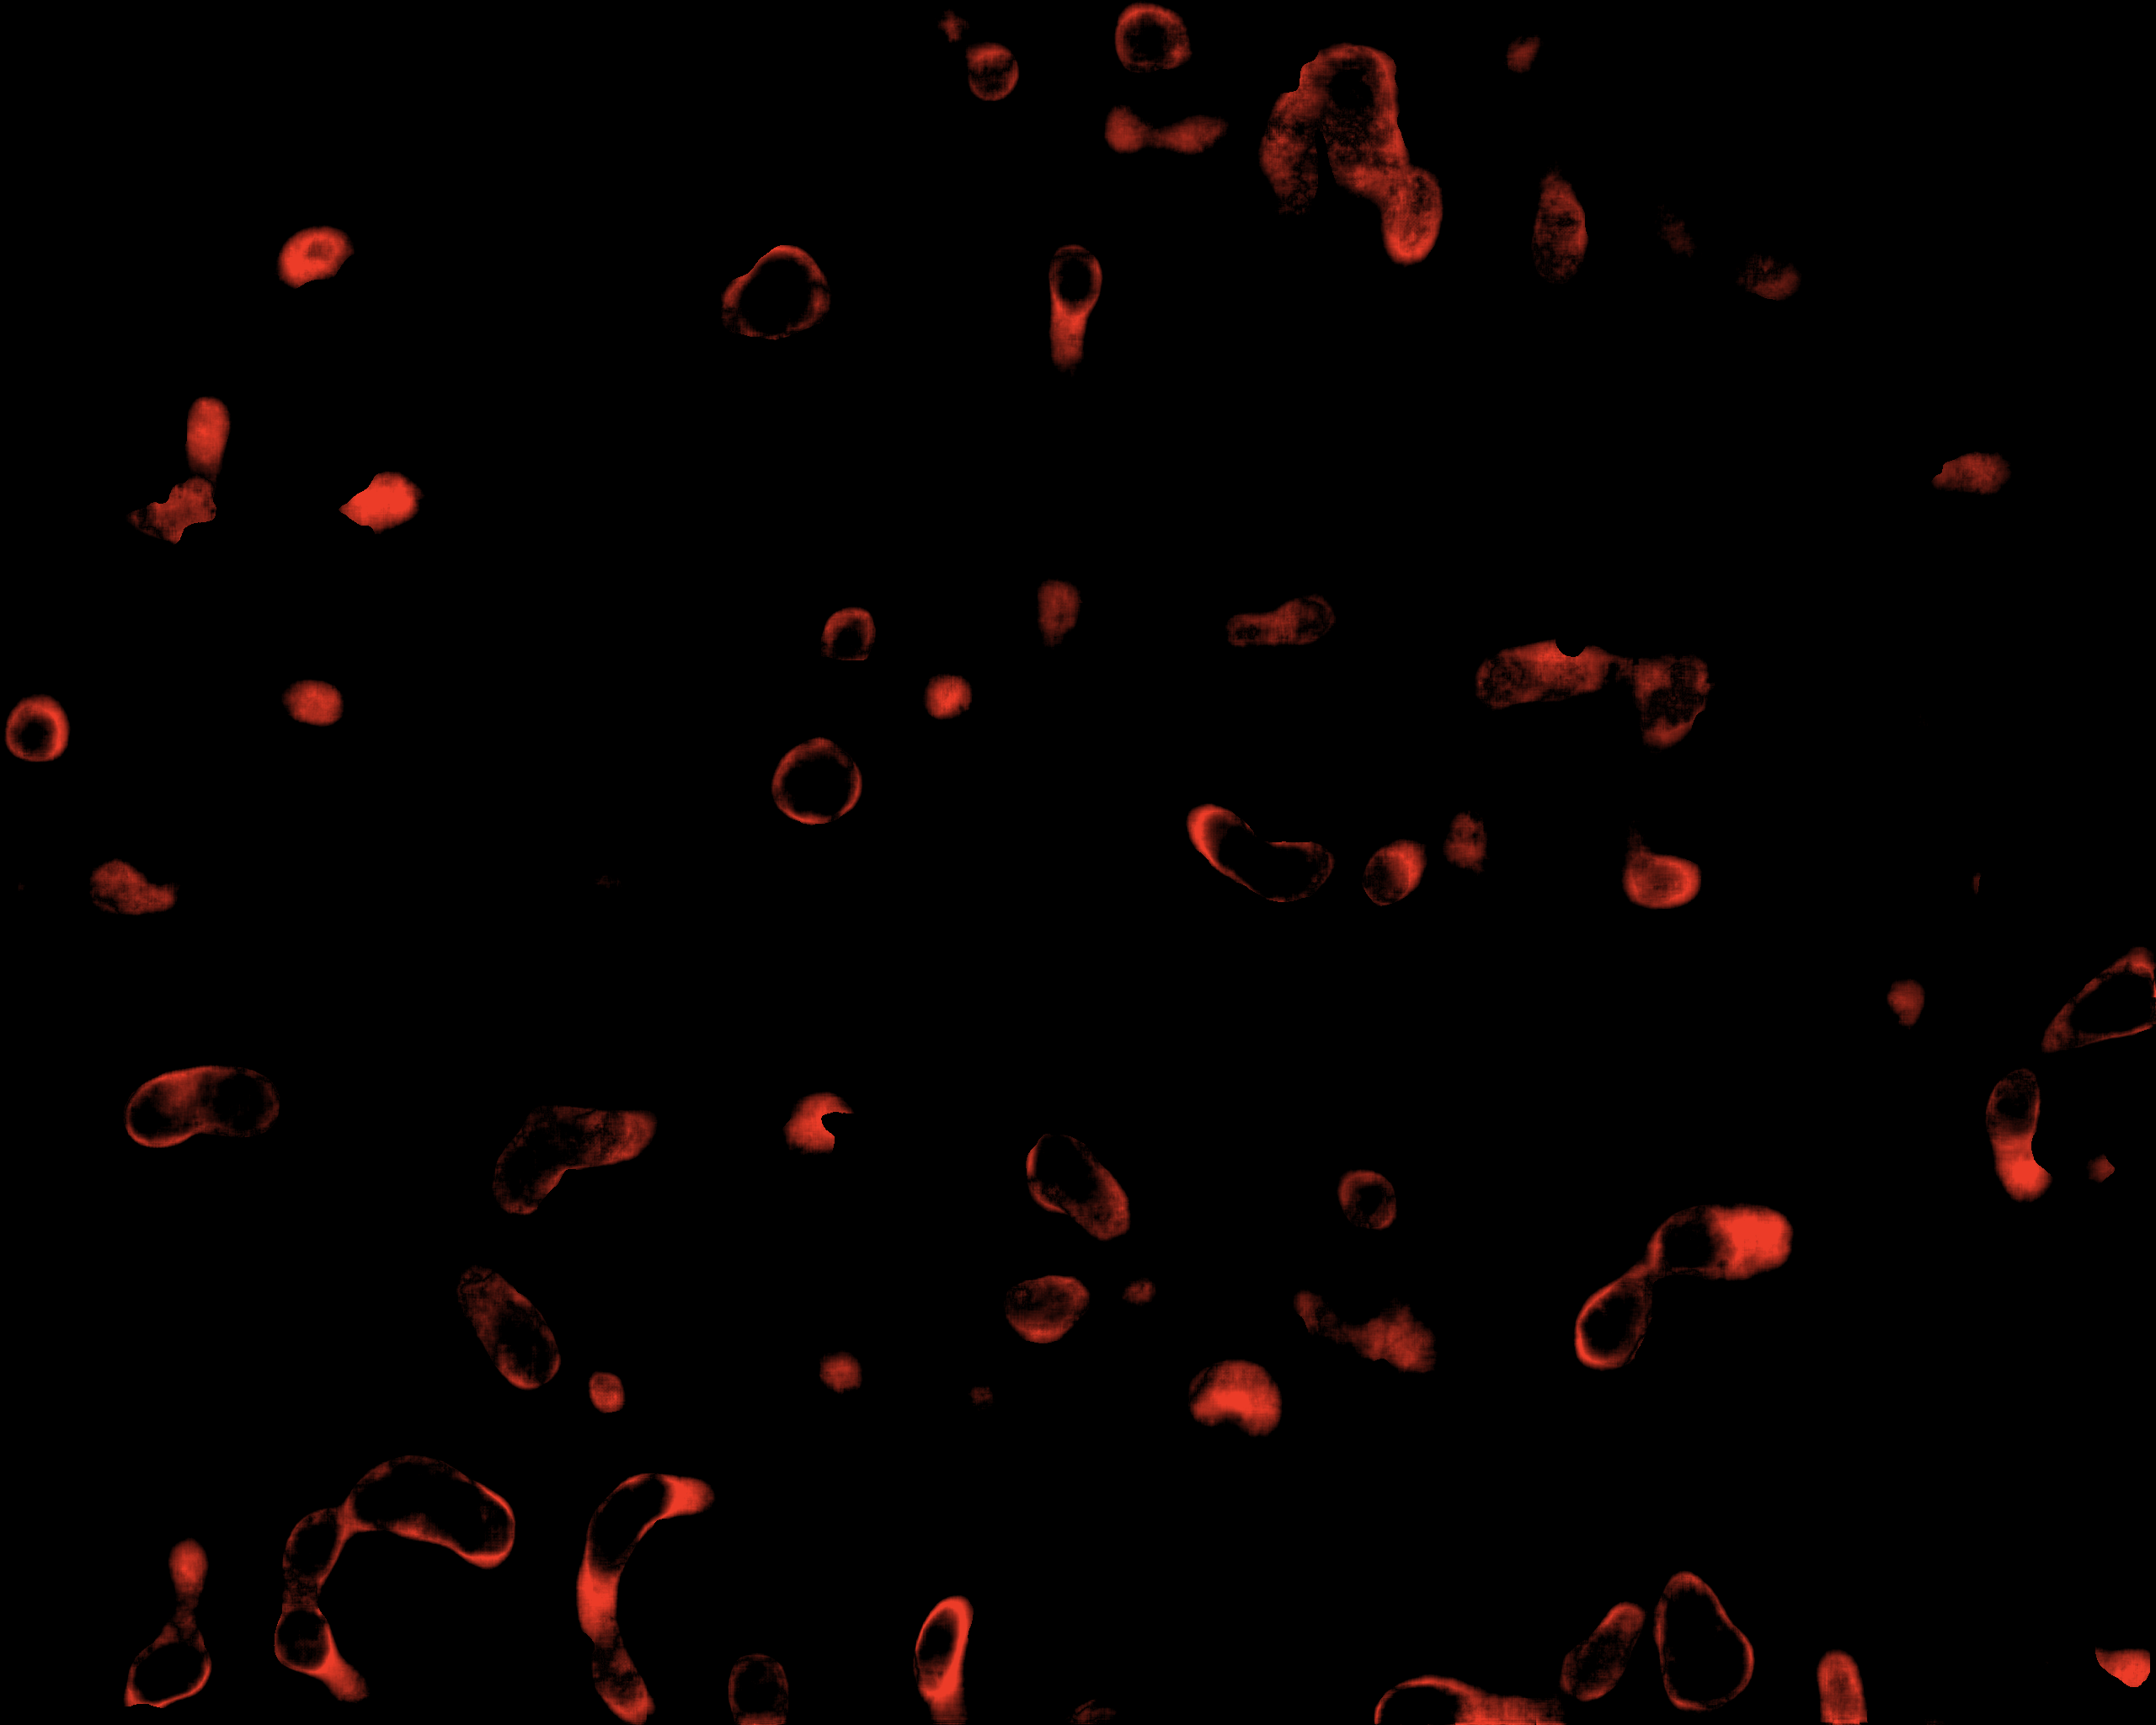
\includegraphics[width=0.29\textwidth]{../figures/m3/20250919125754_3_difference.png}
\caption{Held-out unit 0009B$\cdot$125754. Left, Reader v3 (AUC 0.9562); centre, \MtName{} (AUC 0.9454); right, the red difference between the two maps. Each map is stretched between its own percentiles, the panels are shown at the full resolution of the file.}\label{fig:m3-20250919125754}
\end{figure*}

\begin{figure*}[!tp]
\centering
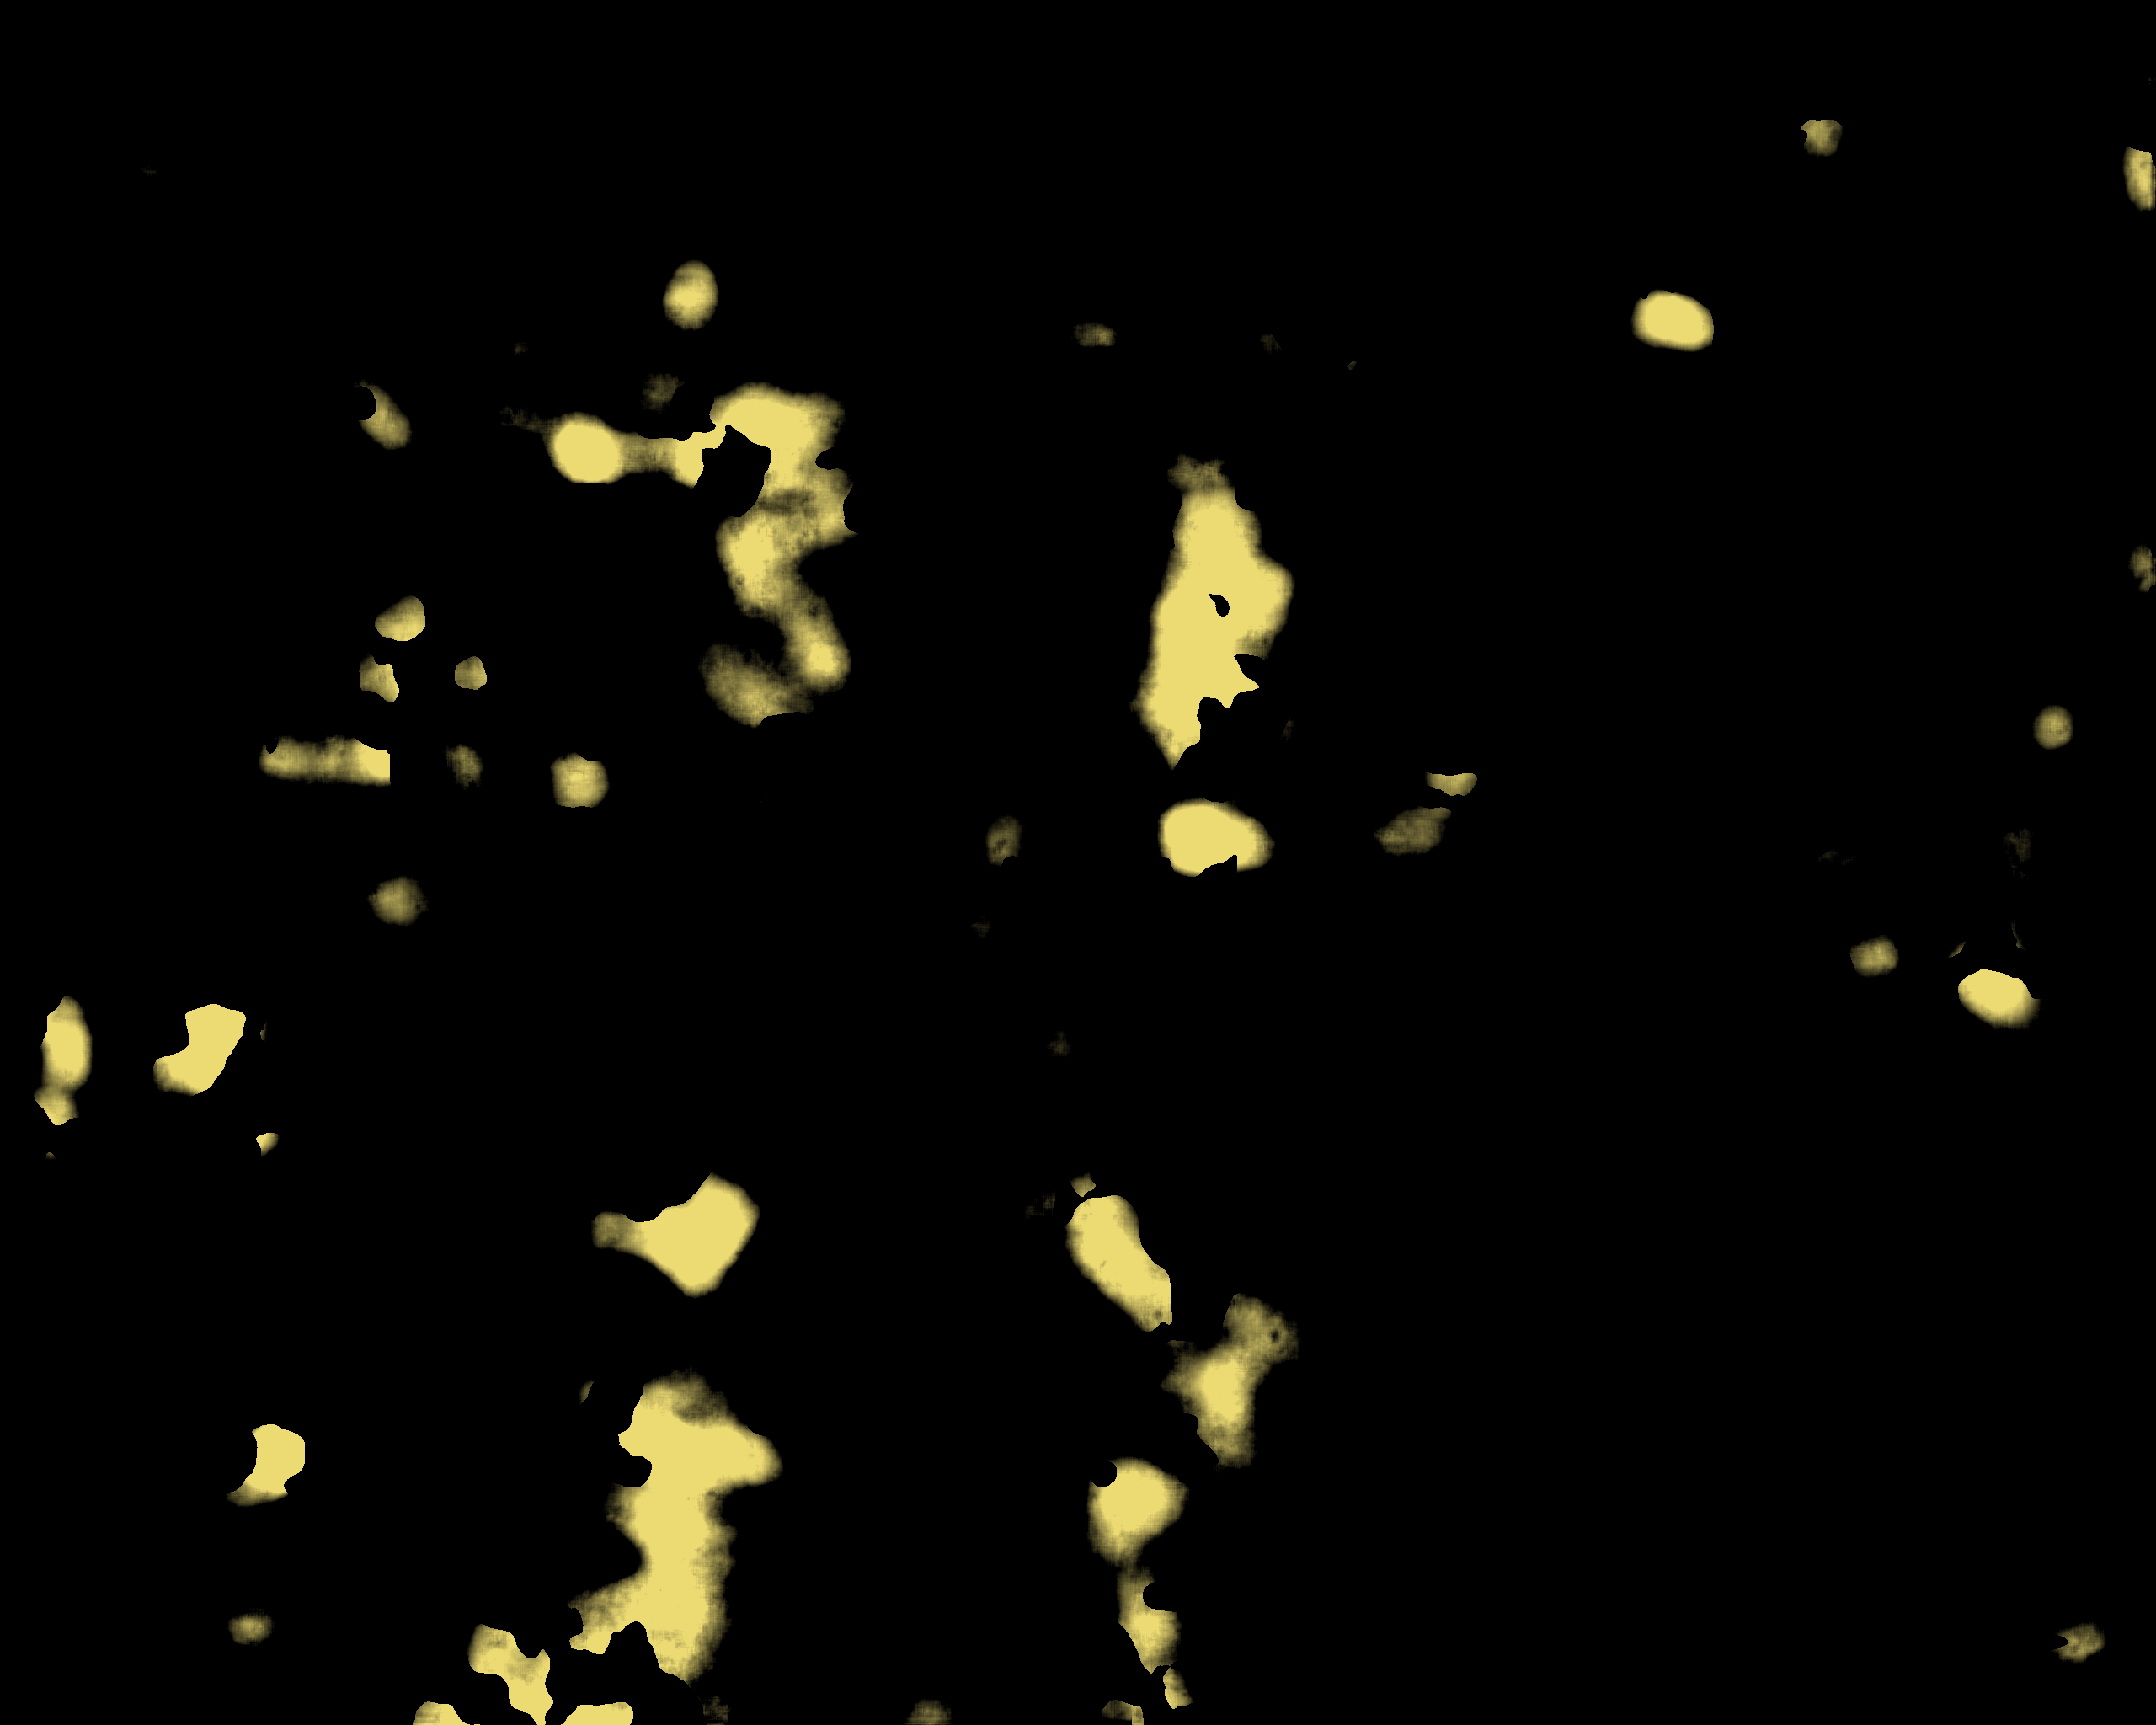
\includegraphics[width=0.29\textwidth]{../figures/m3/20250919133208_1_reader-v3.png}
\hspace{3pt}
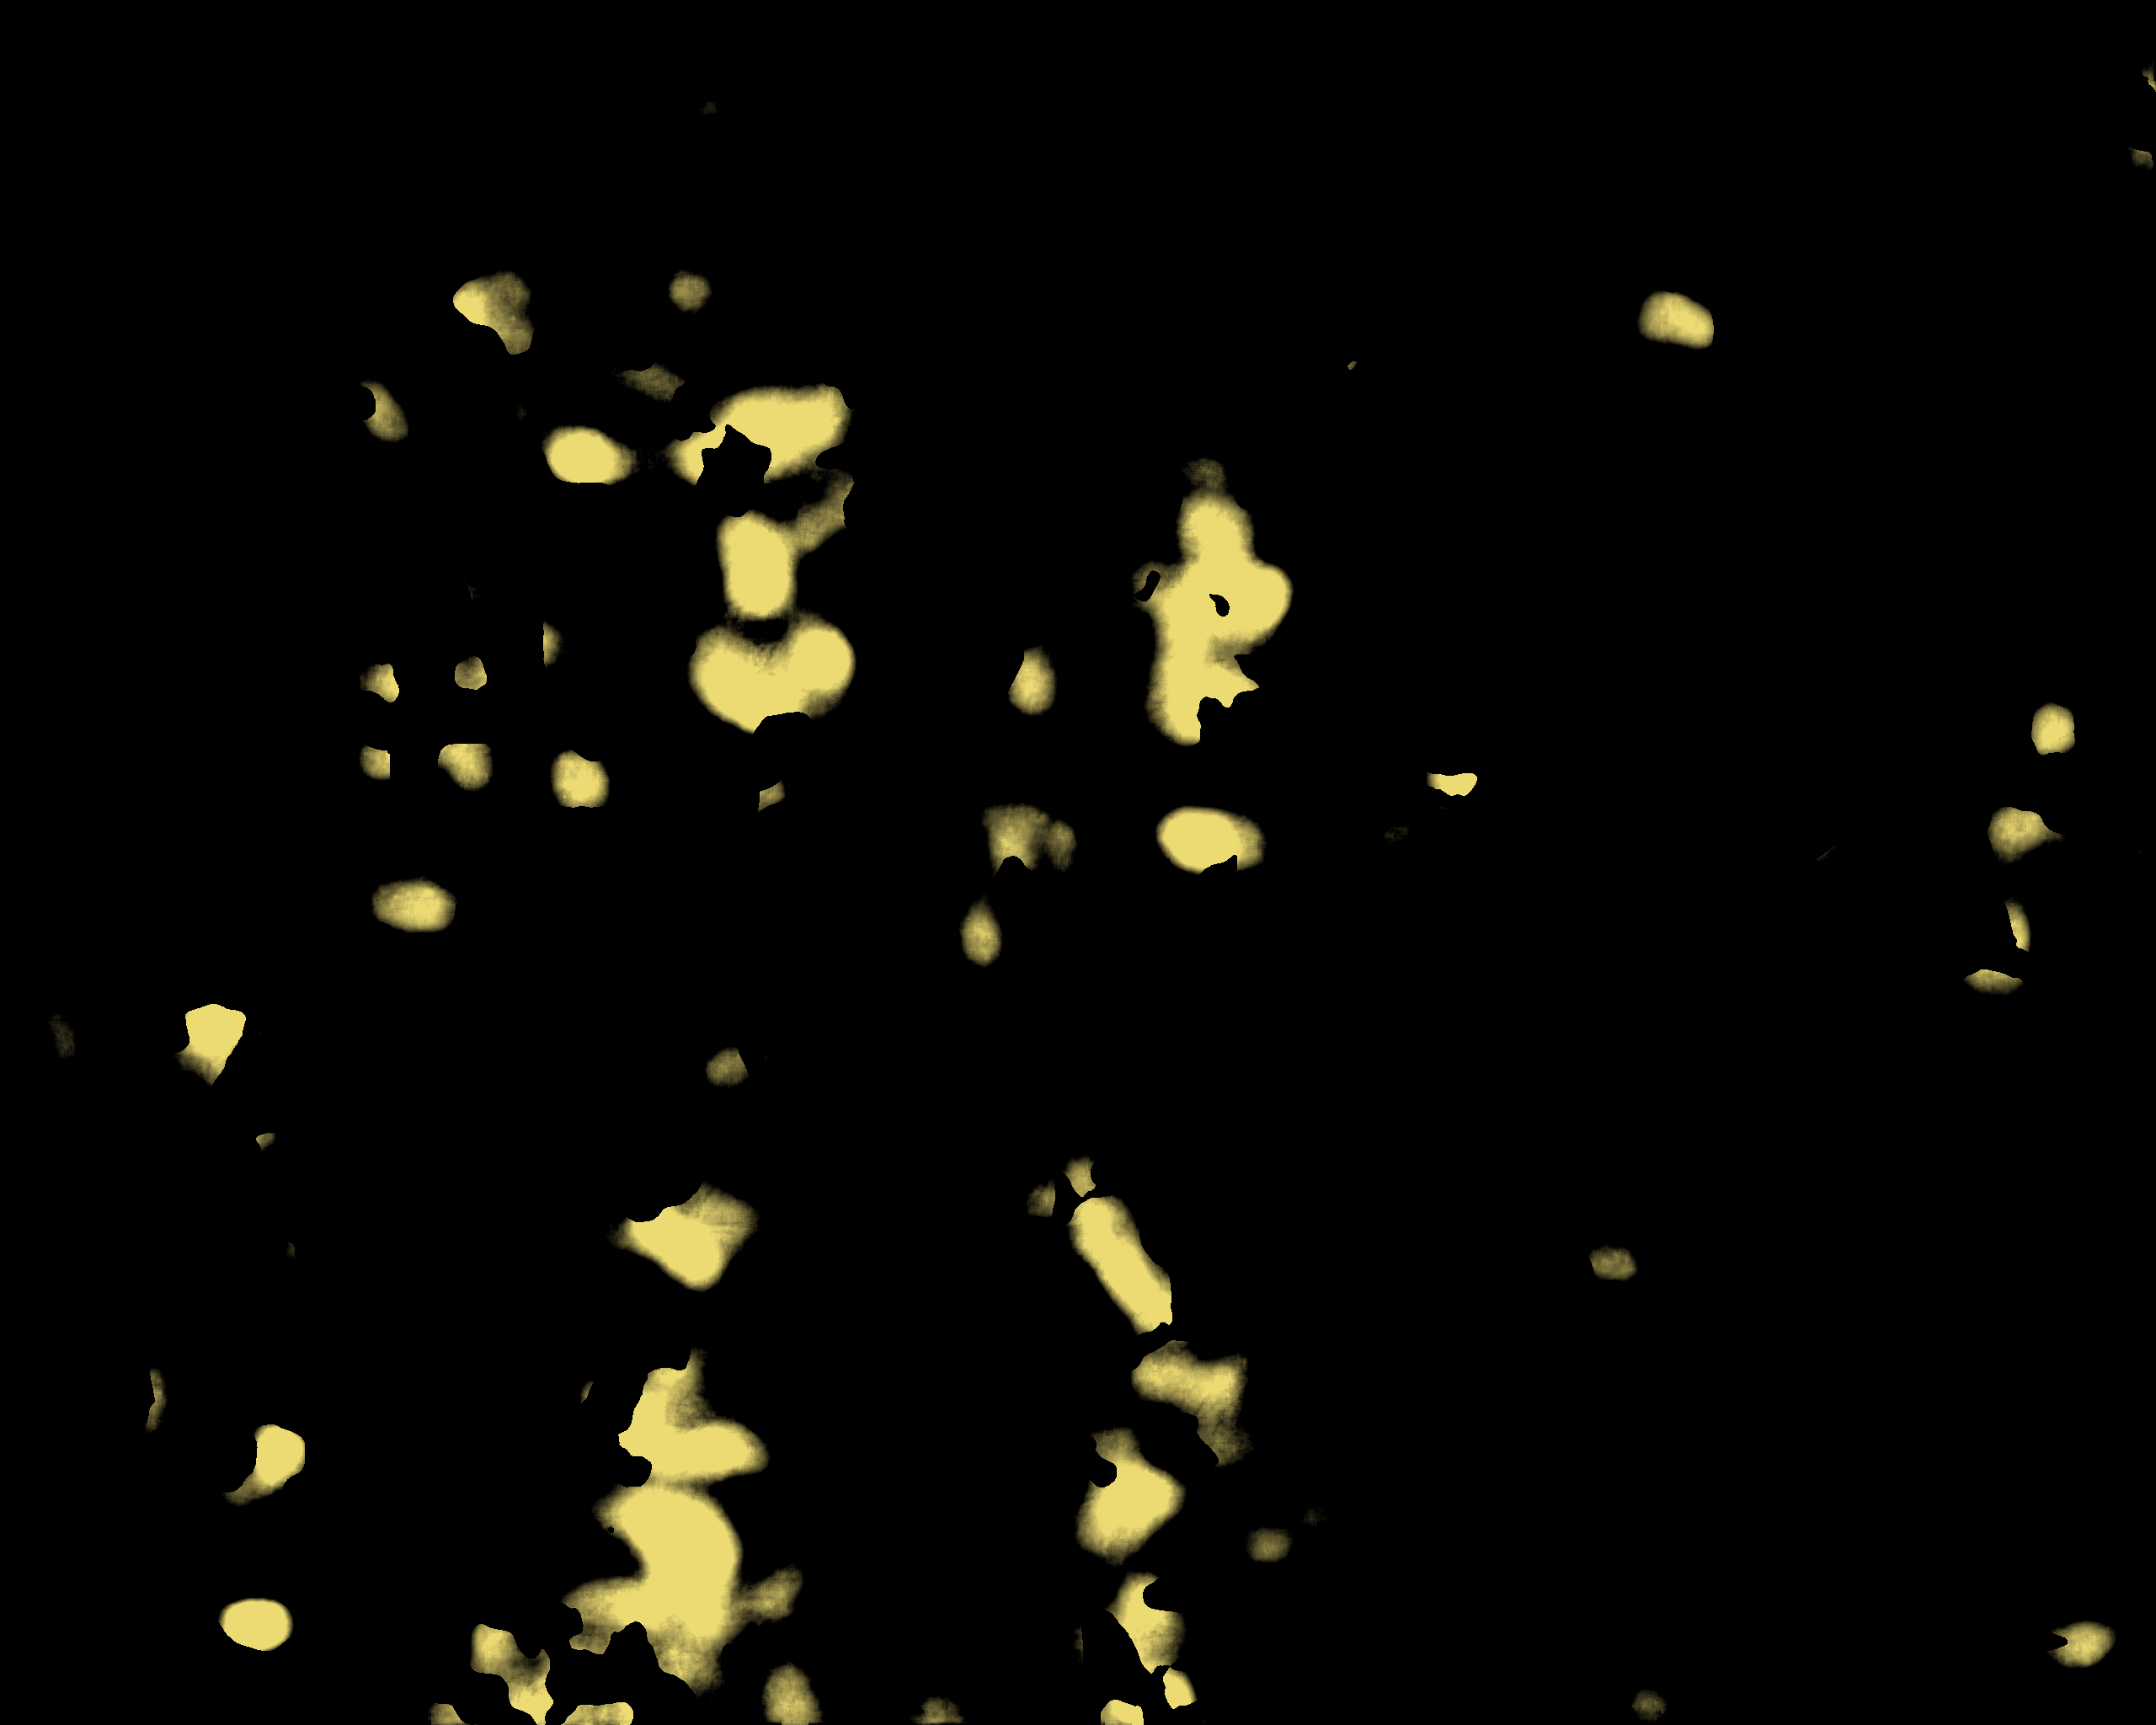
\includegraphics[width=0.29\textwidth]{../figures/m3/20250919133208_2_m3.png}
\hspace{3pt}
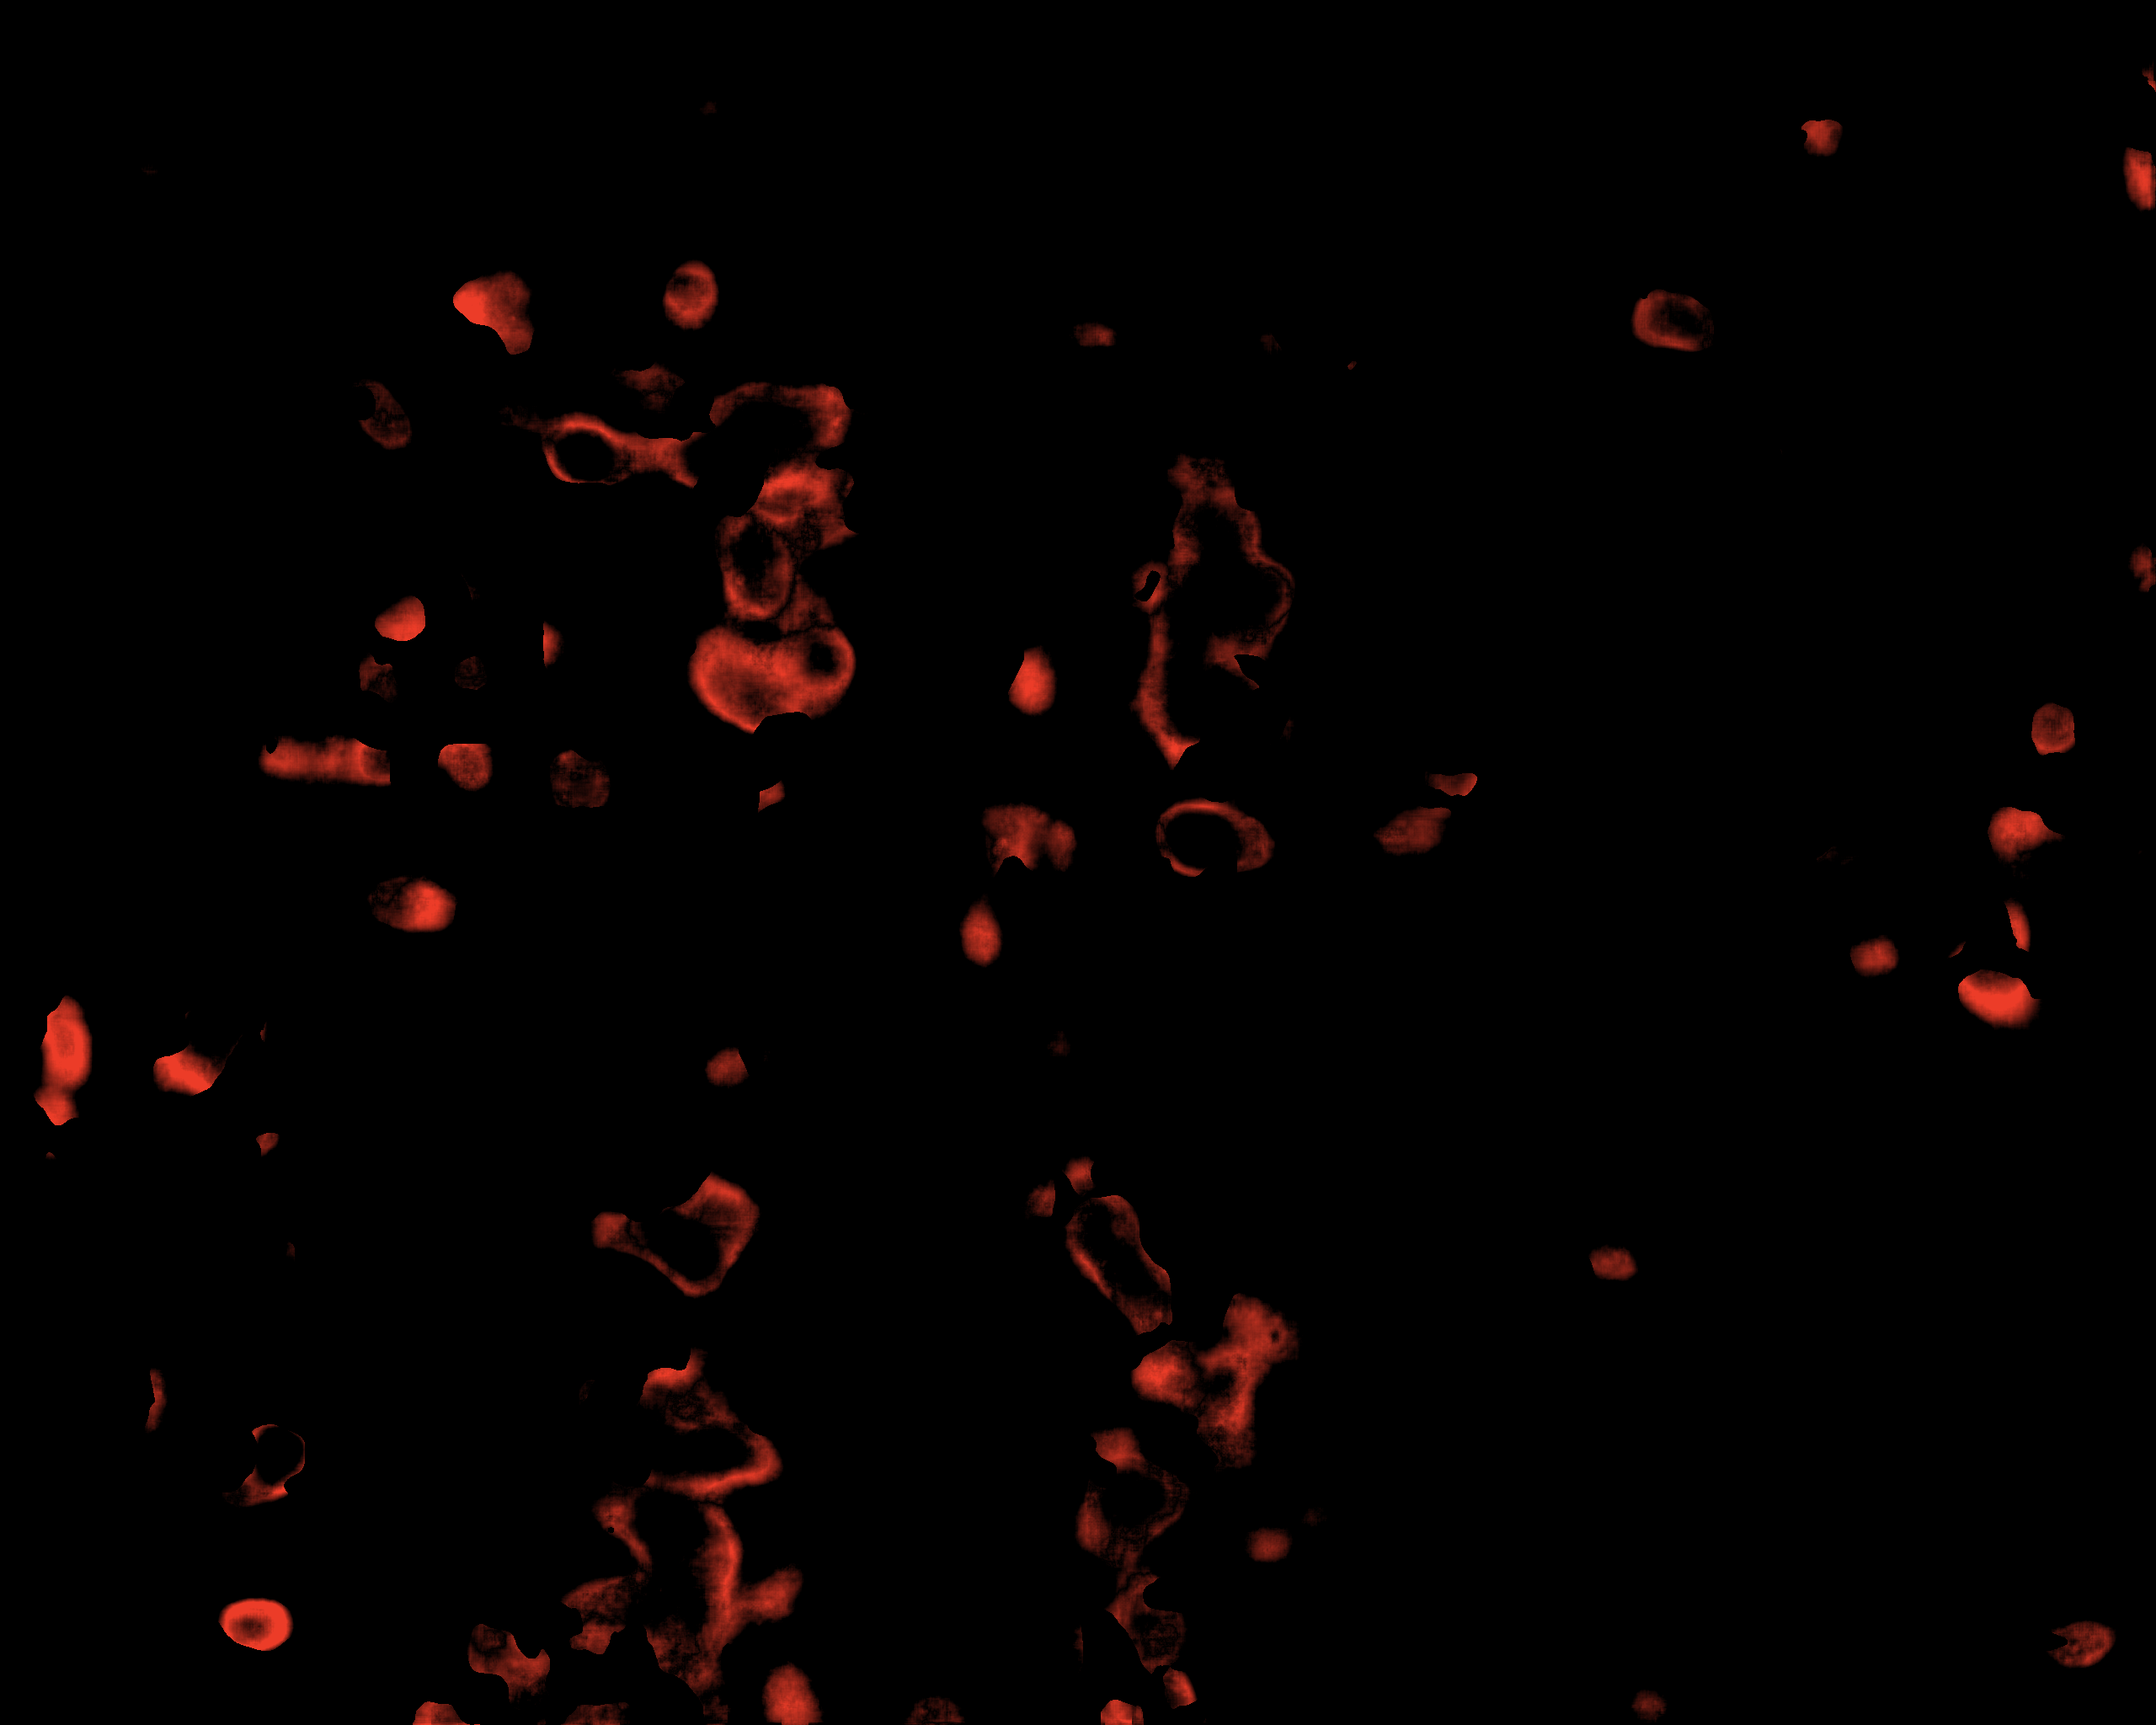
\includegraphics[width=0.29\textwidth]{../figures/m3/20250919133208_3_difference.png}
\caption{Held-out unit 0009B$\cdot$133208. Left, Reader v3 (AUC 0.8551); centre, \MtName{} (AUC 0.8658); right, the red difference between the two maps. Each map is stretched between its own percentiles, the panels are shown at the full resolution of the file.}\label{fig:m3-20250919133208}
\end{figure*}

\begin{figure*}[!tp]
\centering
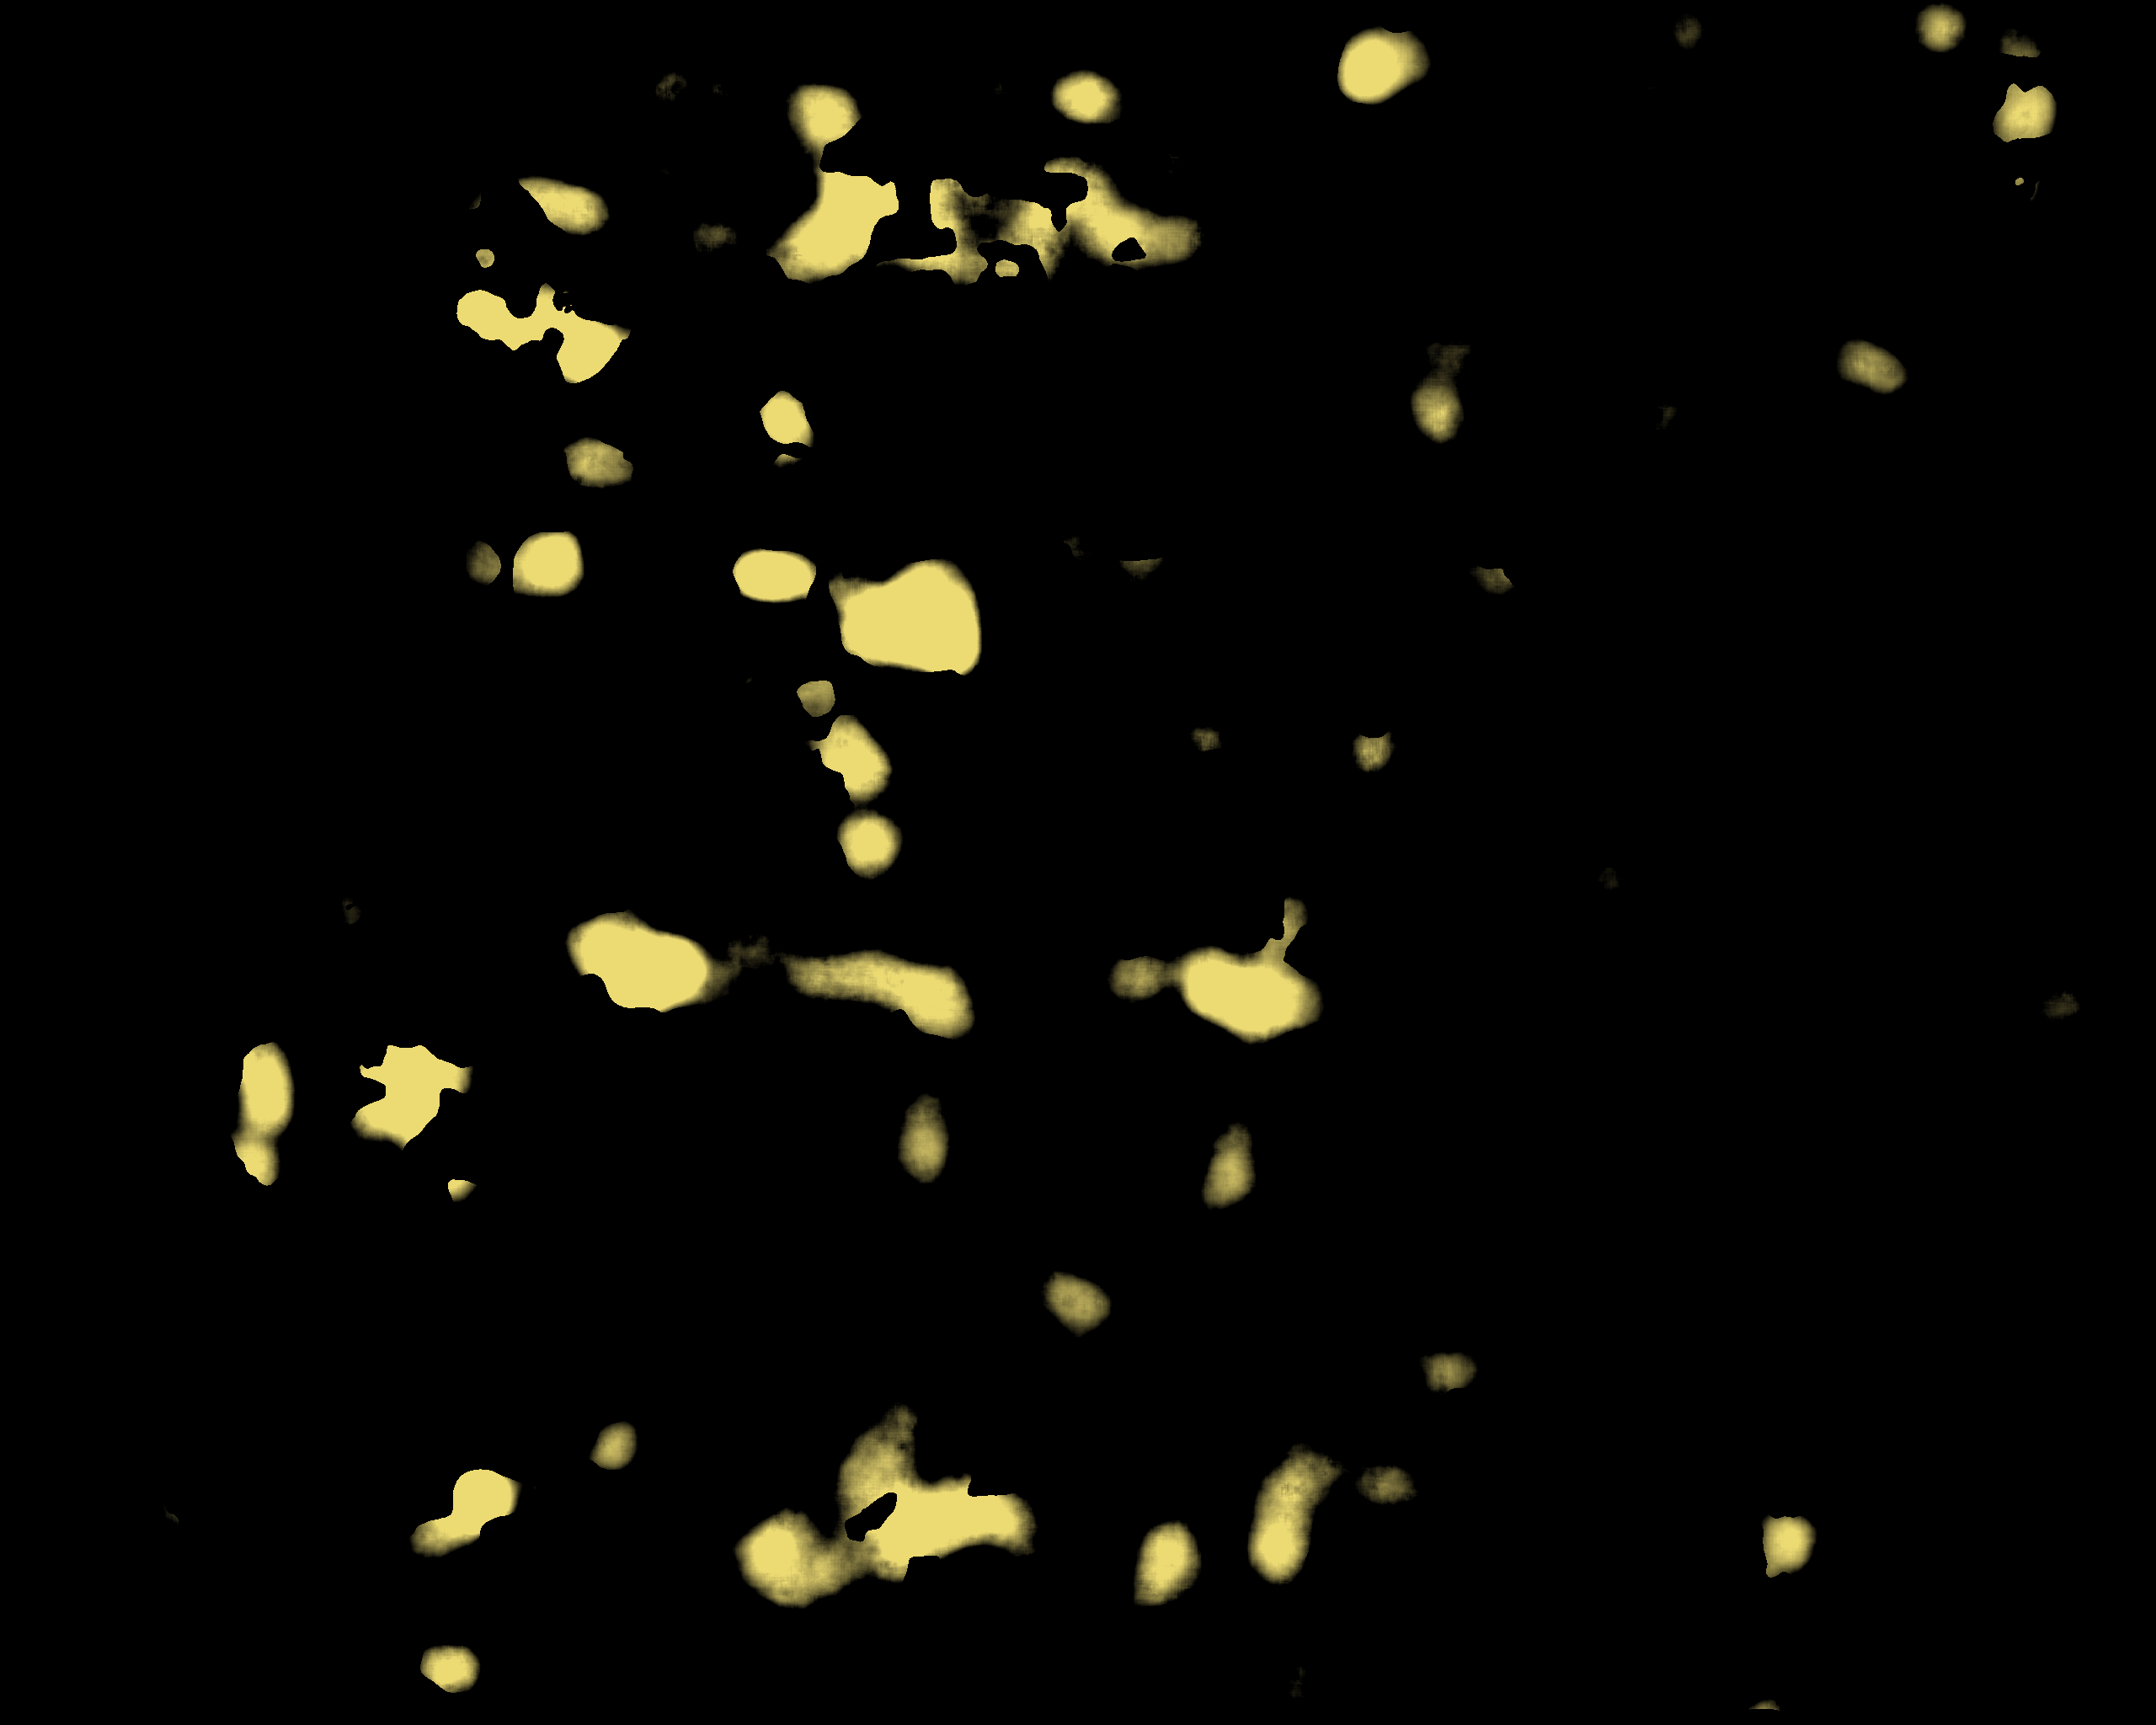
\includegraphics[width=0.29\textwidth]{../figures/m3/20250919140325_1_reader-v3.png}
\hspace{3pt}
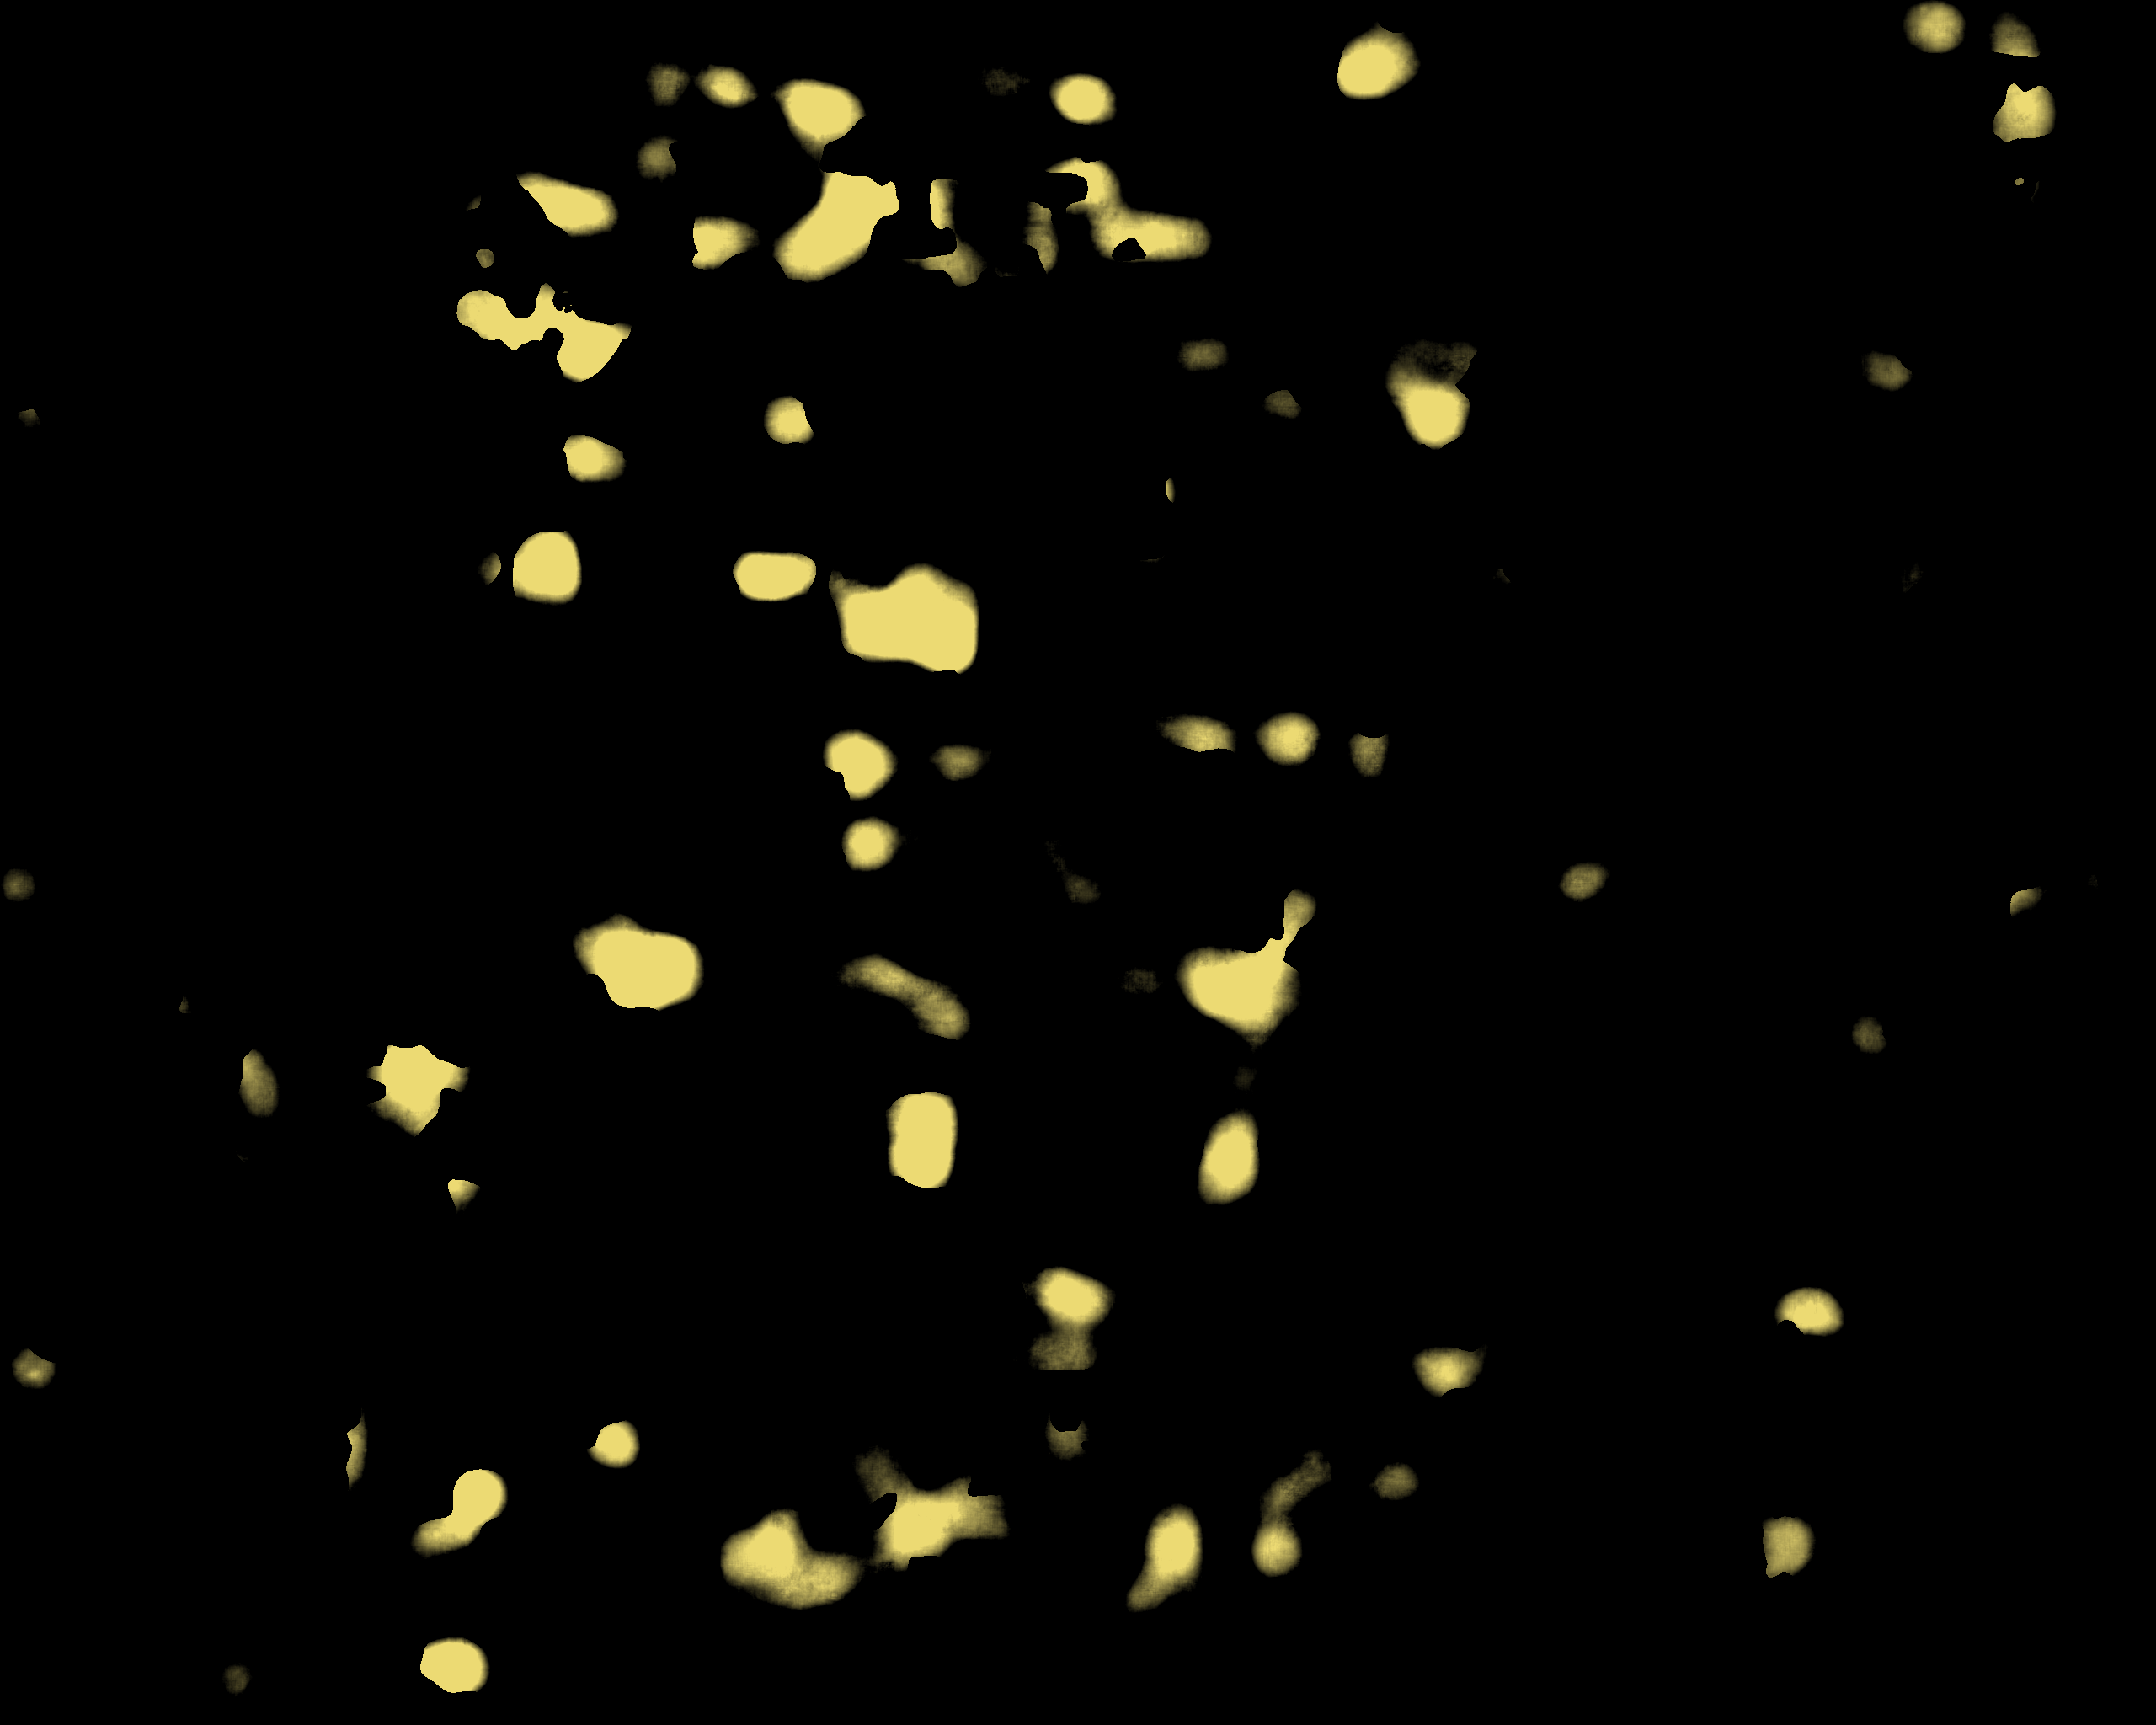
\includegraphics[width=0.29\textwidth]{../figures/m3/20250919140325_2_m3.png}
\hspace{3pt}
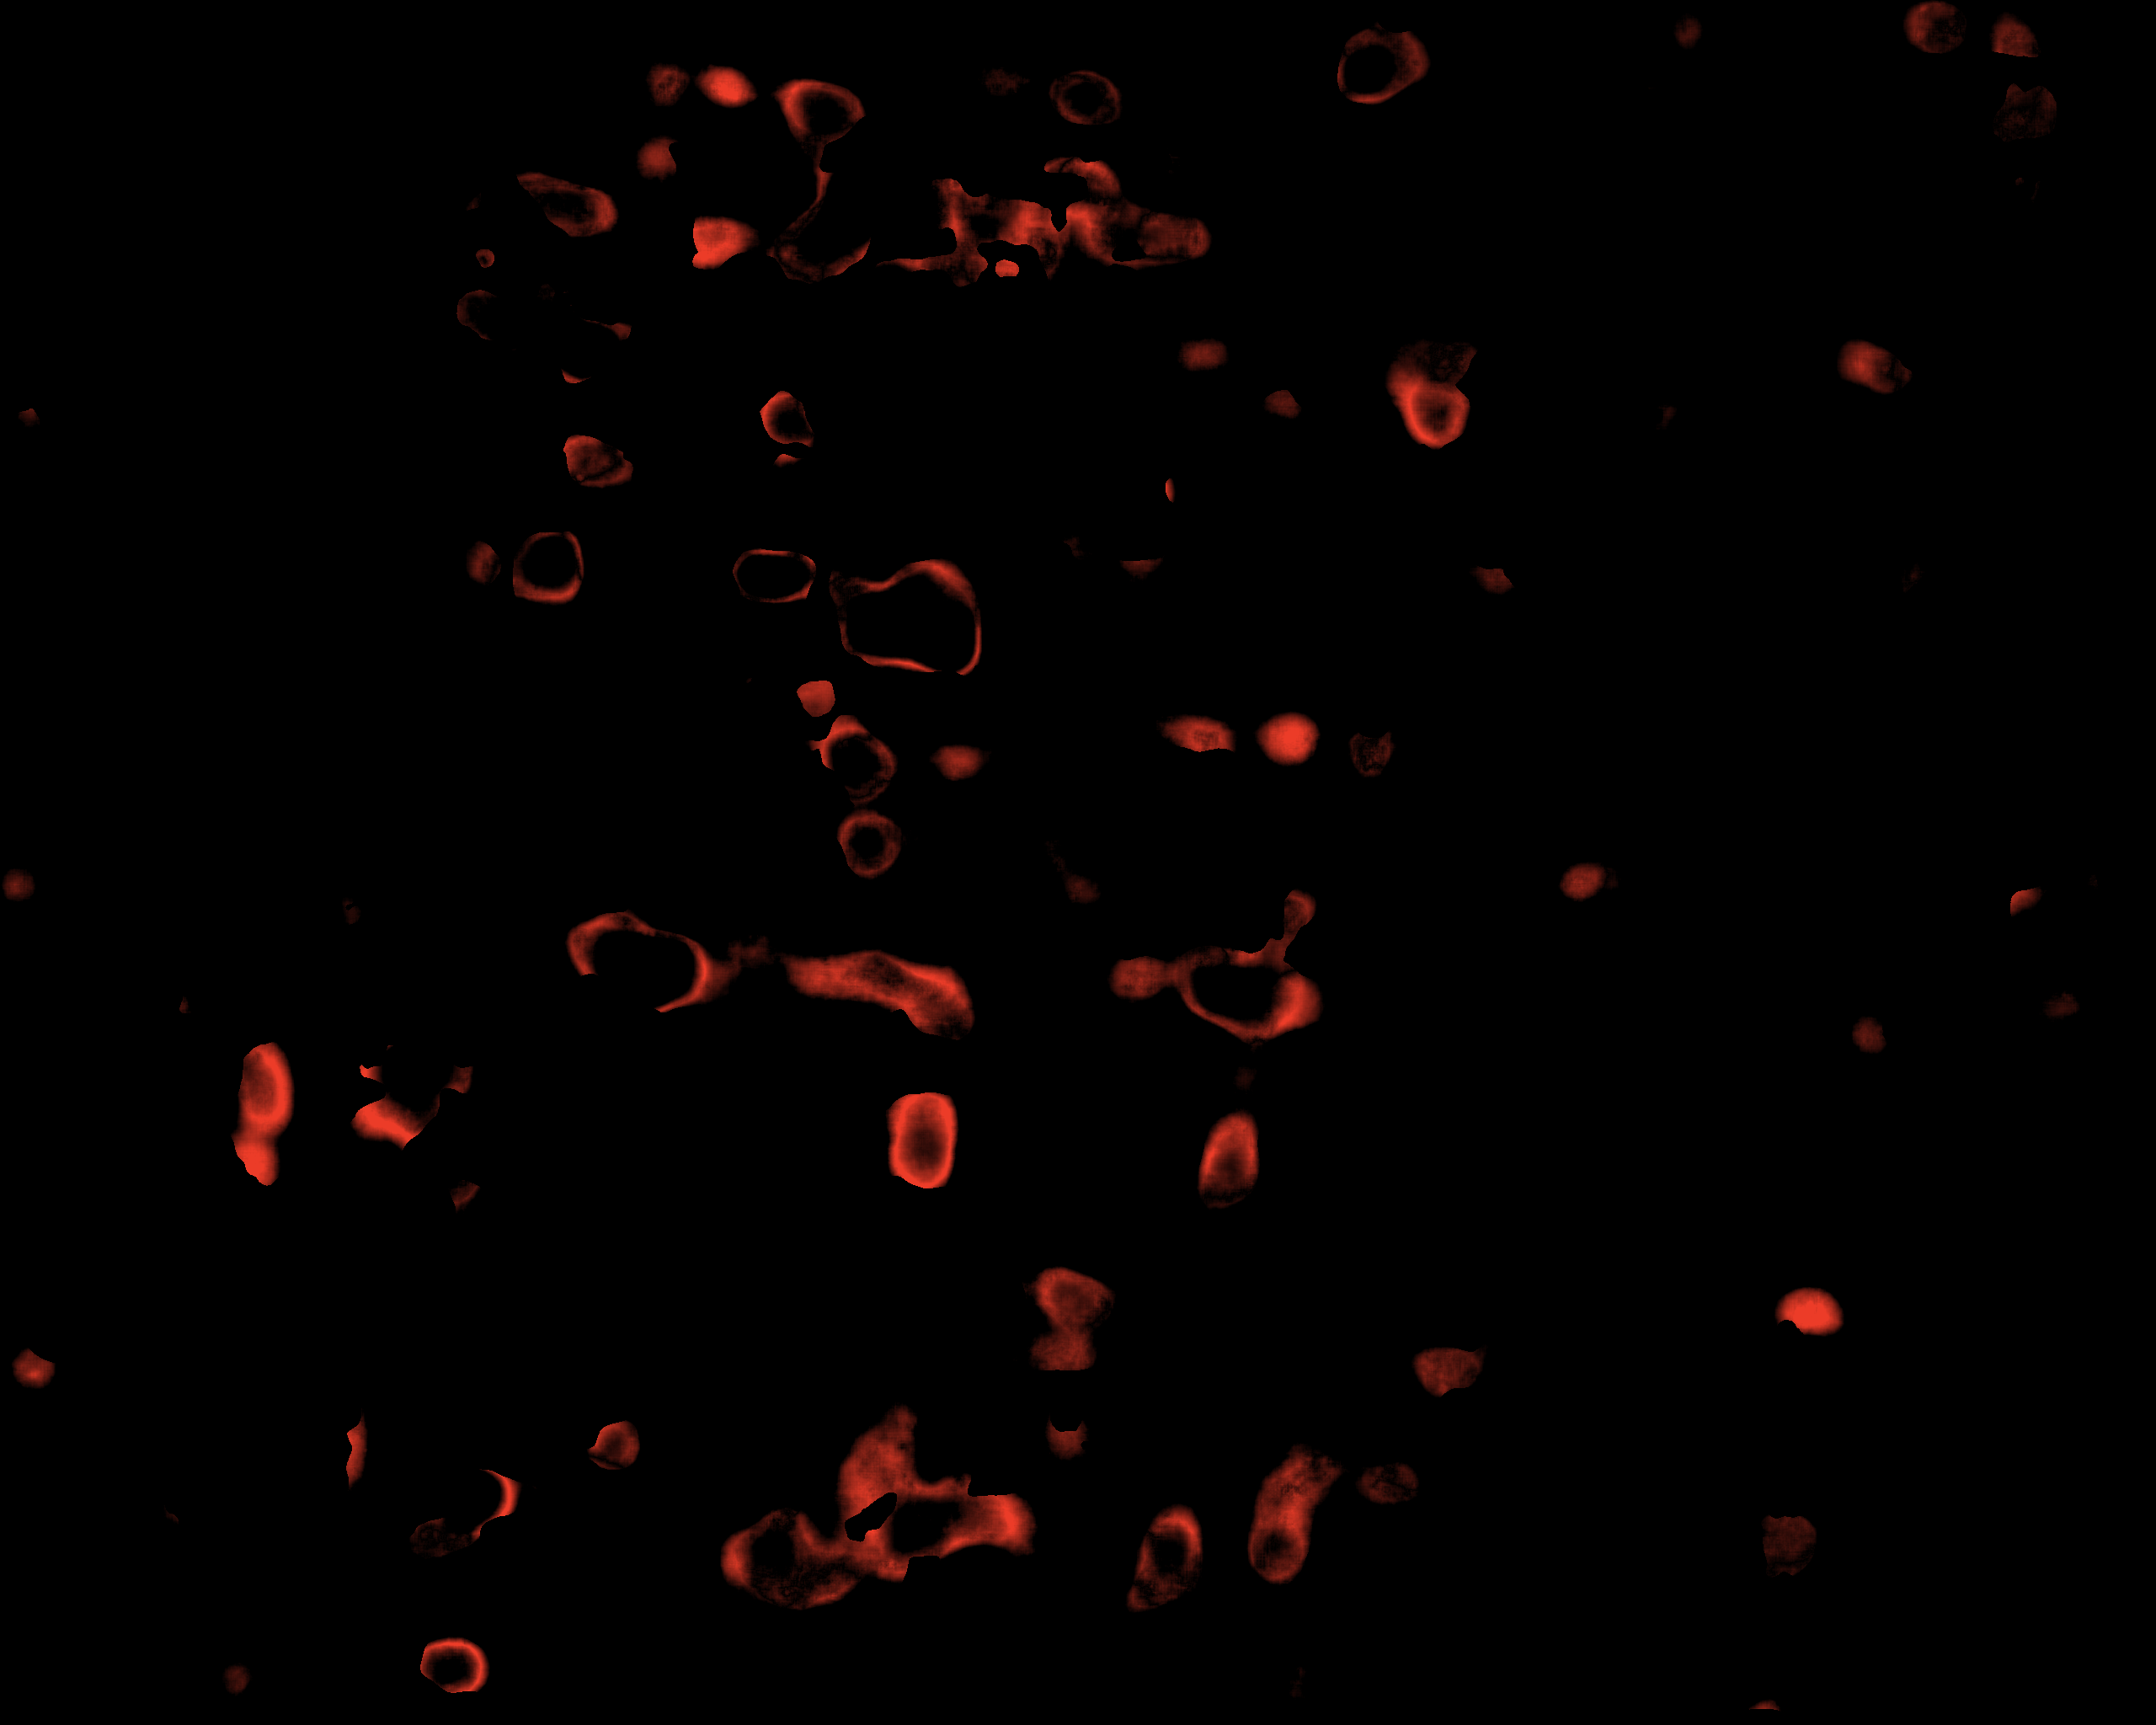
\includegraphics[width=0.29\textwidth]{../figures/m3/20250919140325_3_difference.png}
\caption{Held-out unit 0009B$\cdot$140325. Left, Reader v3 (AUC 0.9040); centre, \MtName{} (AUC 0.8761); right, the red difference between the two maps. Each map is stretched between its own percentiles, the panels are shown at the full resolution of the file.}\label{fig:m3-20250919140325}
\end{figure*}

\begin{figure*}[!tp]
\centering
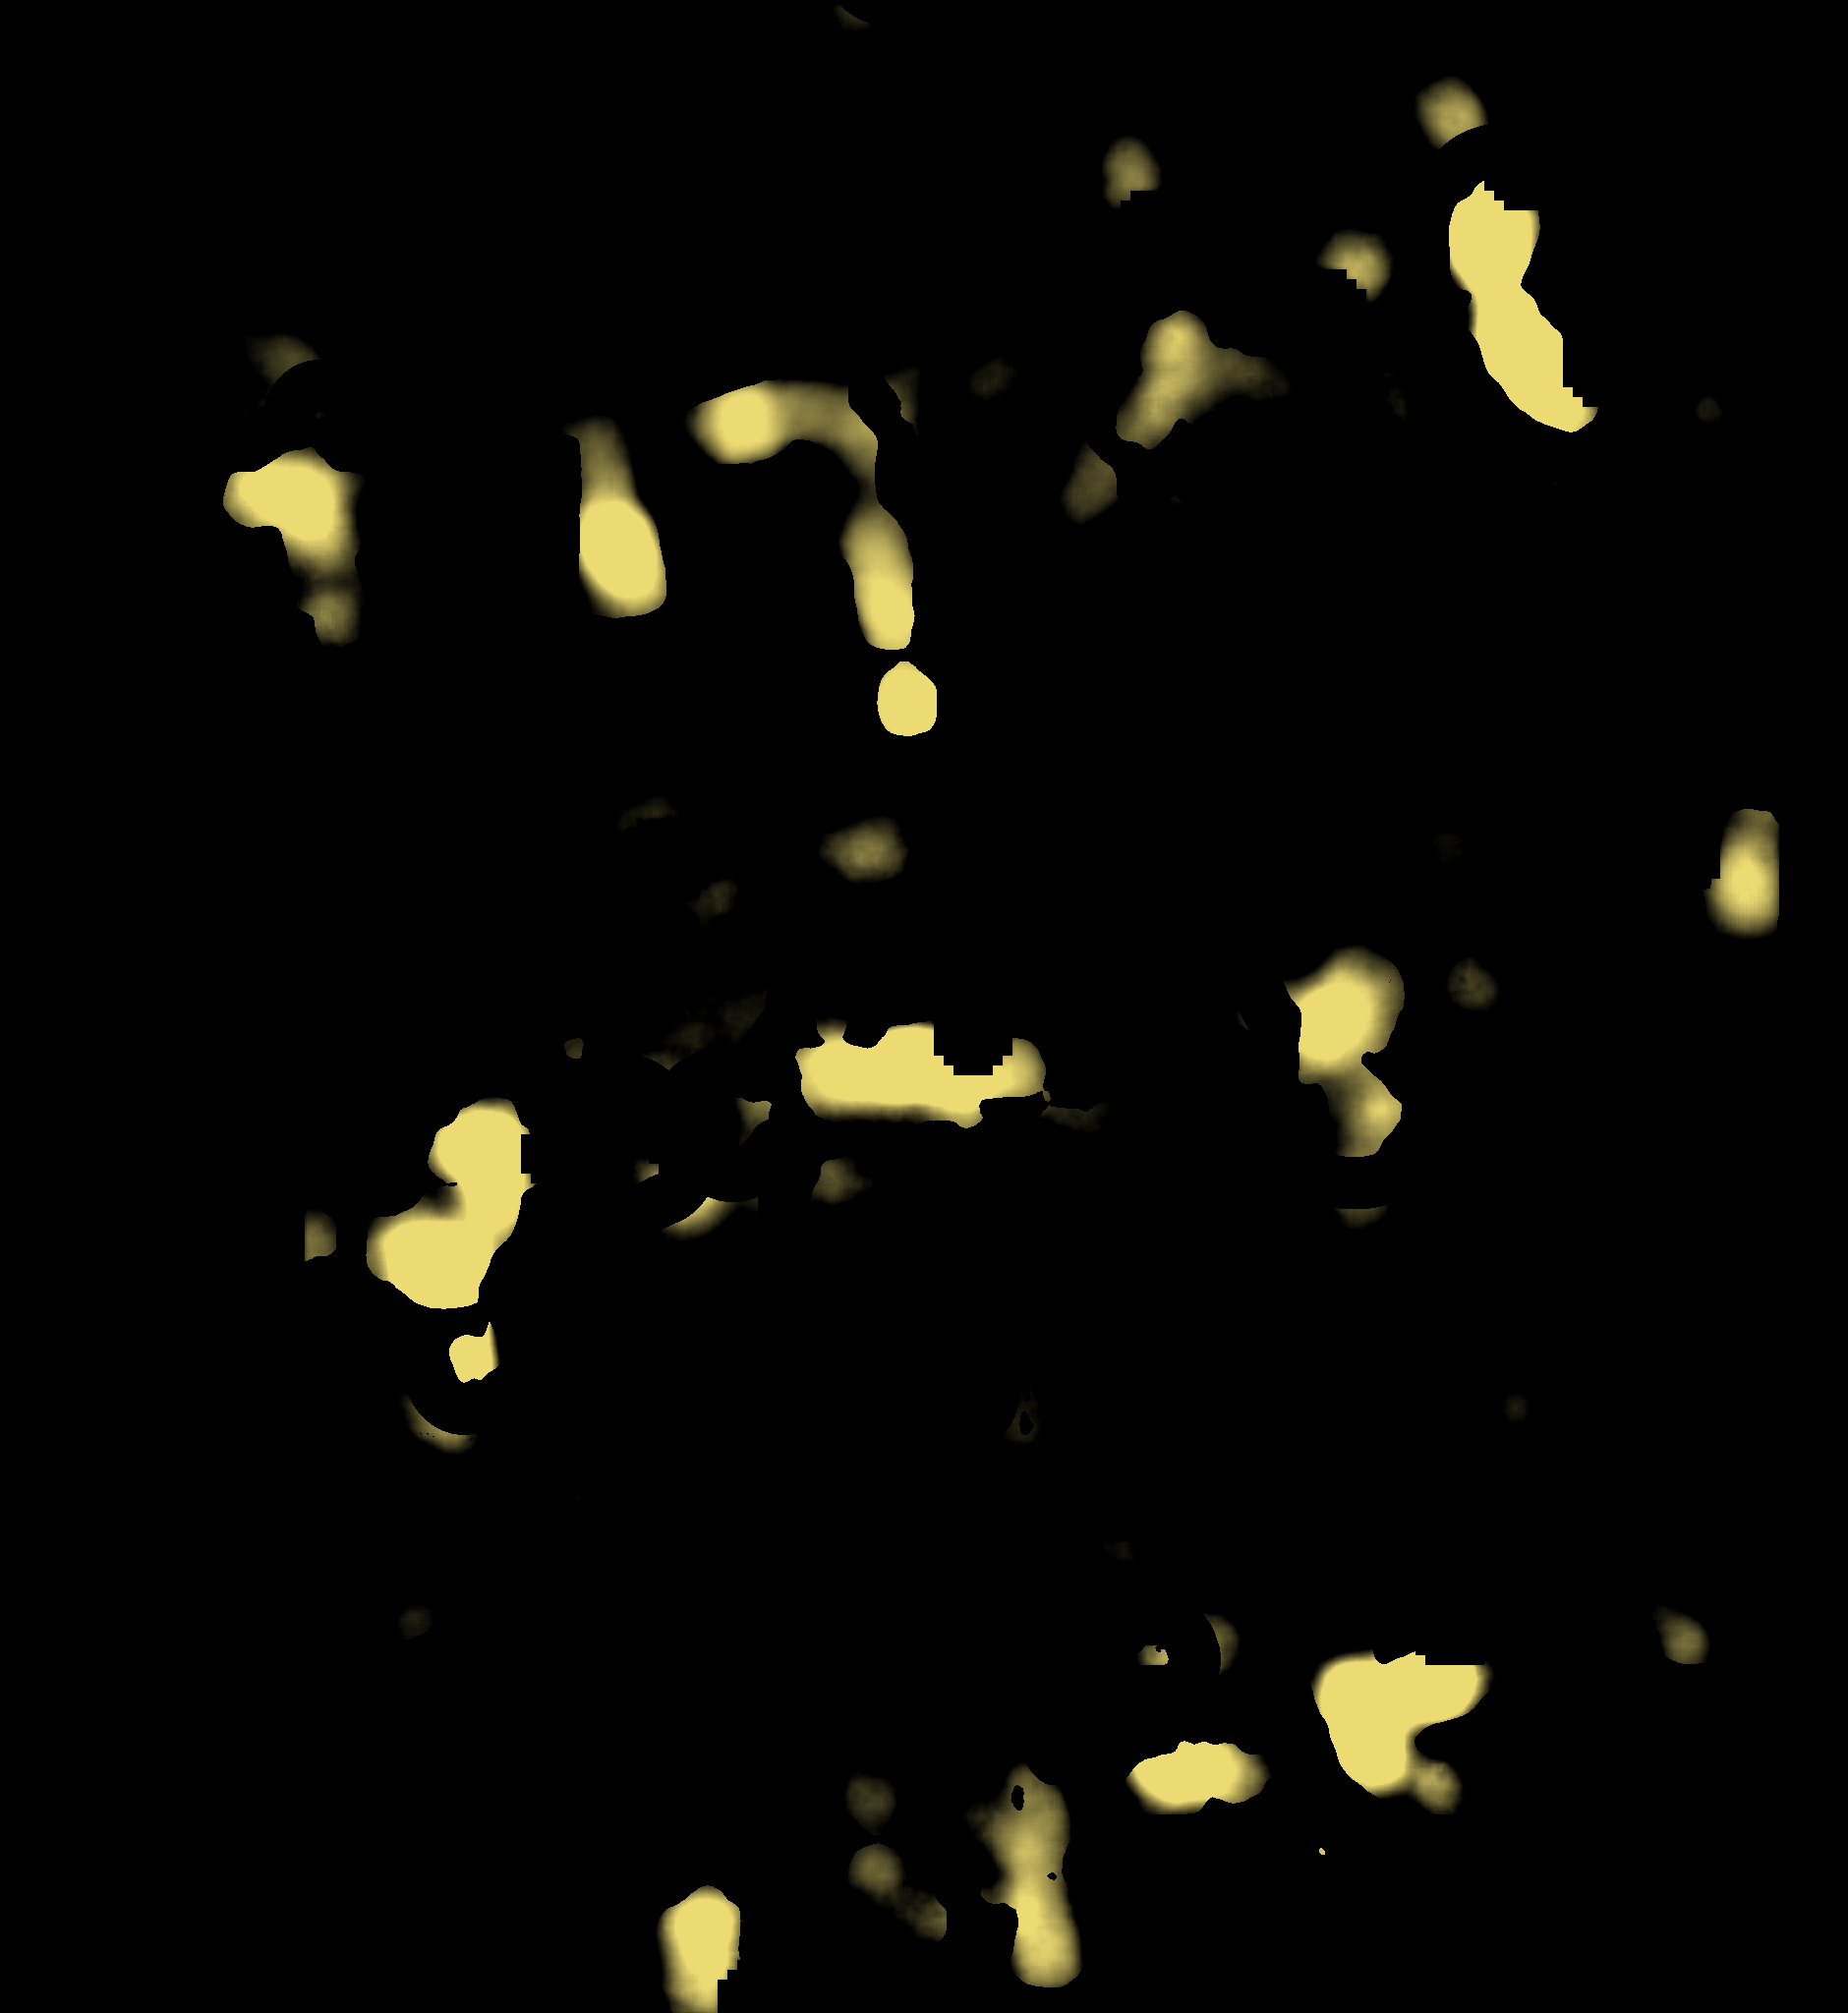
\includegraphics[width=0.29\textwidth]{../figures/m3/20250716055229_1_reader-v3.png}
\hspace{3pt}
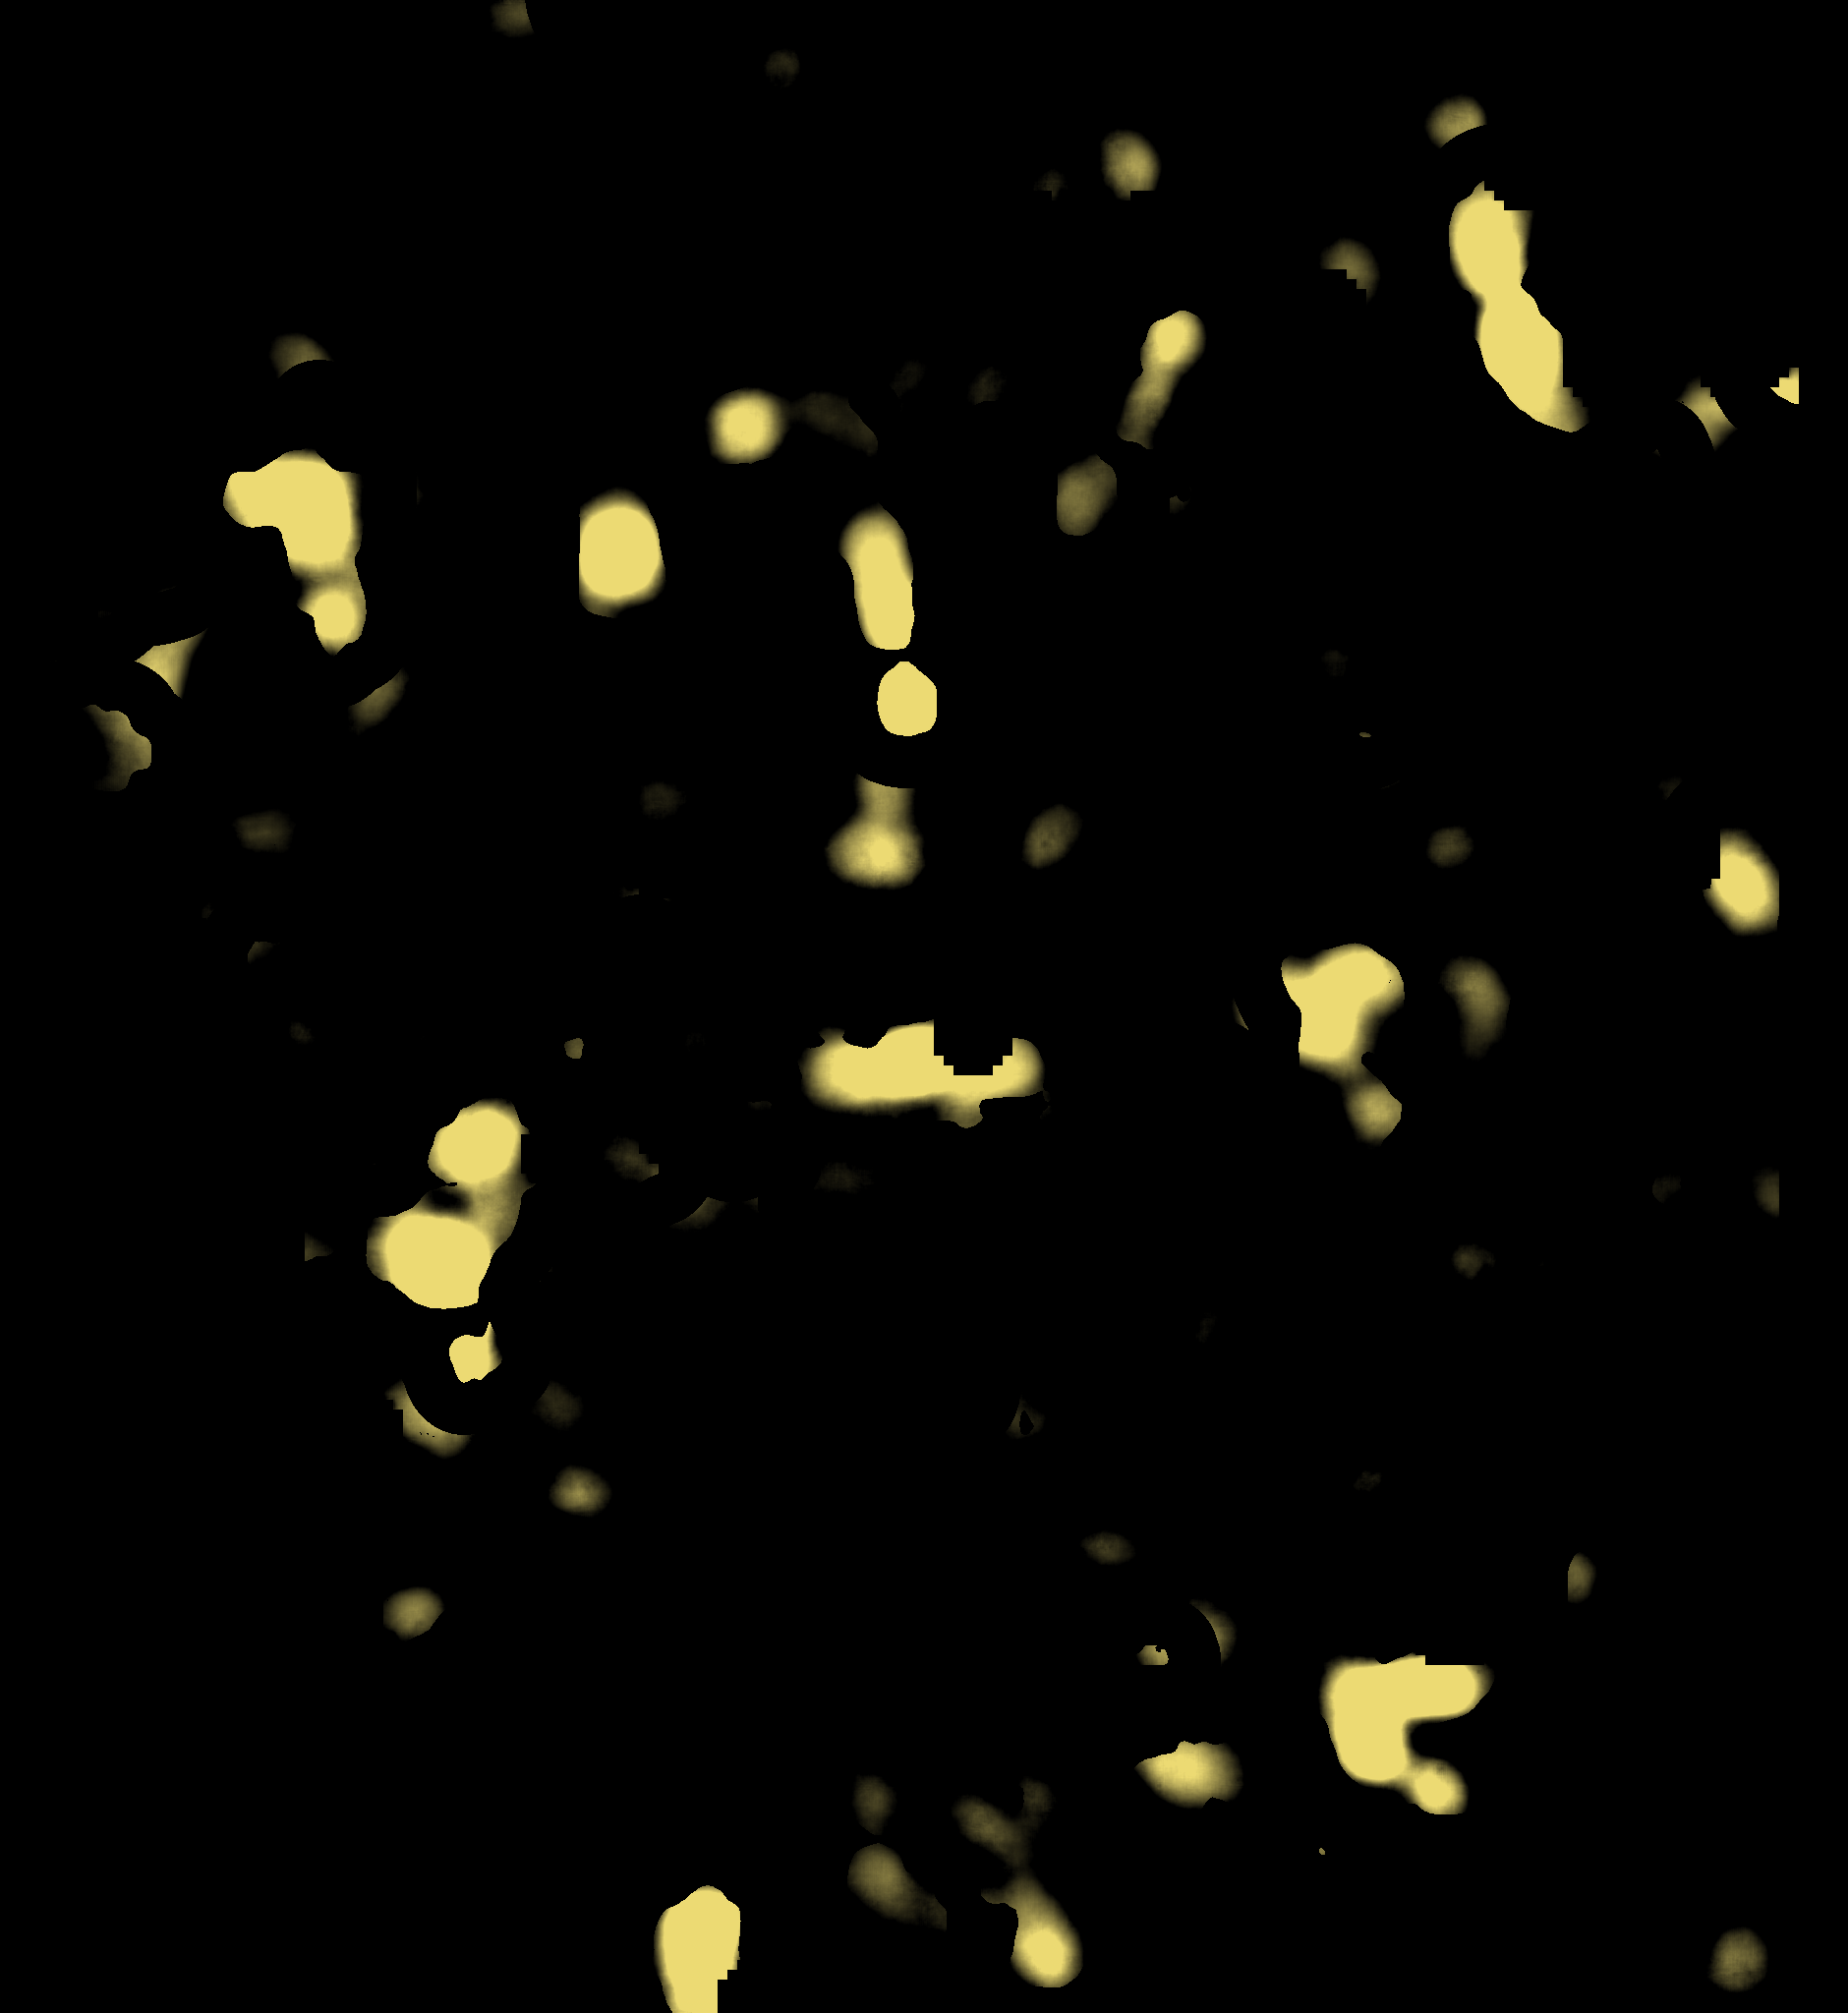
\includegraphics[width=0.29\textwidth]{../figures/m3/20250716055229_2_m3.png}
\hspace{3pt}
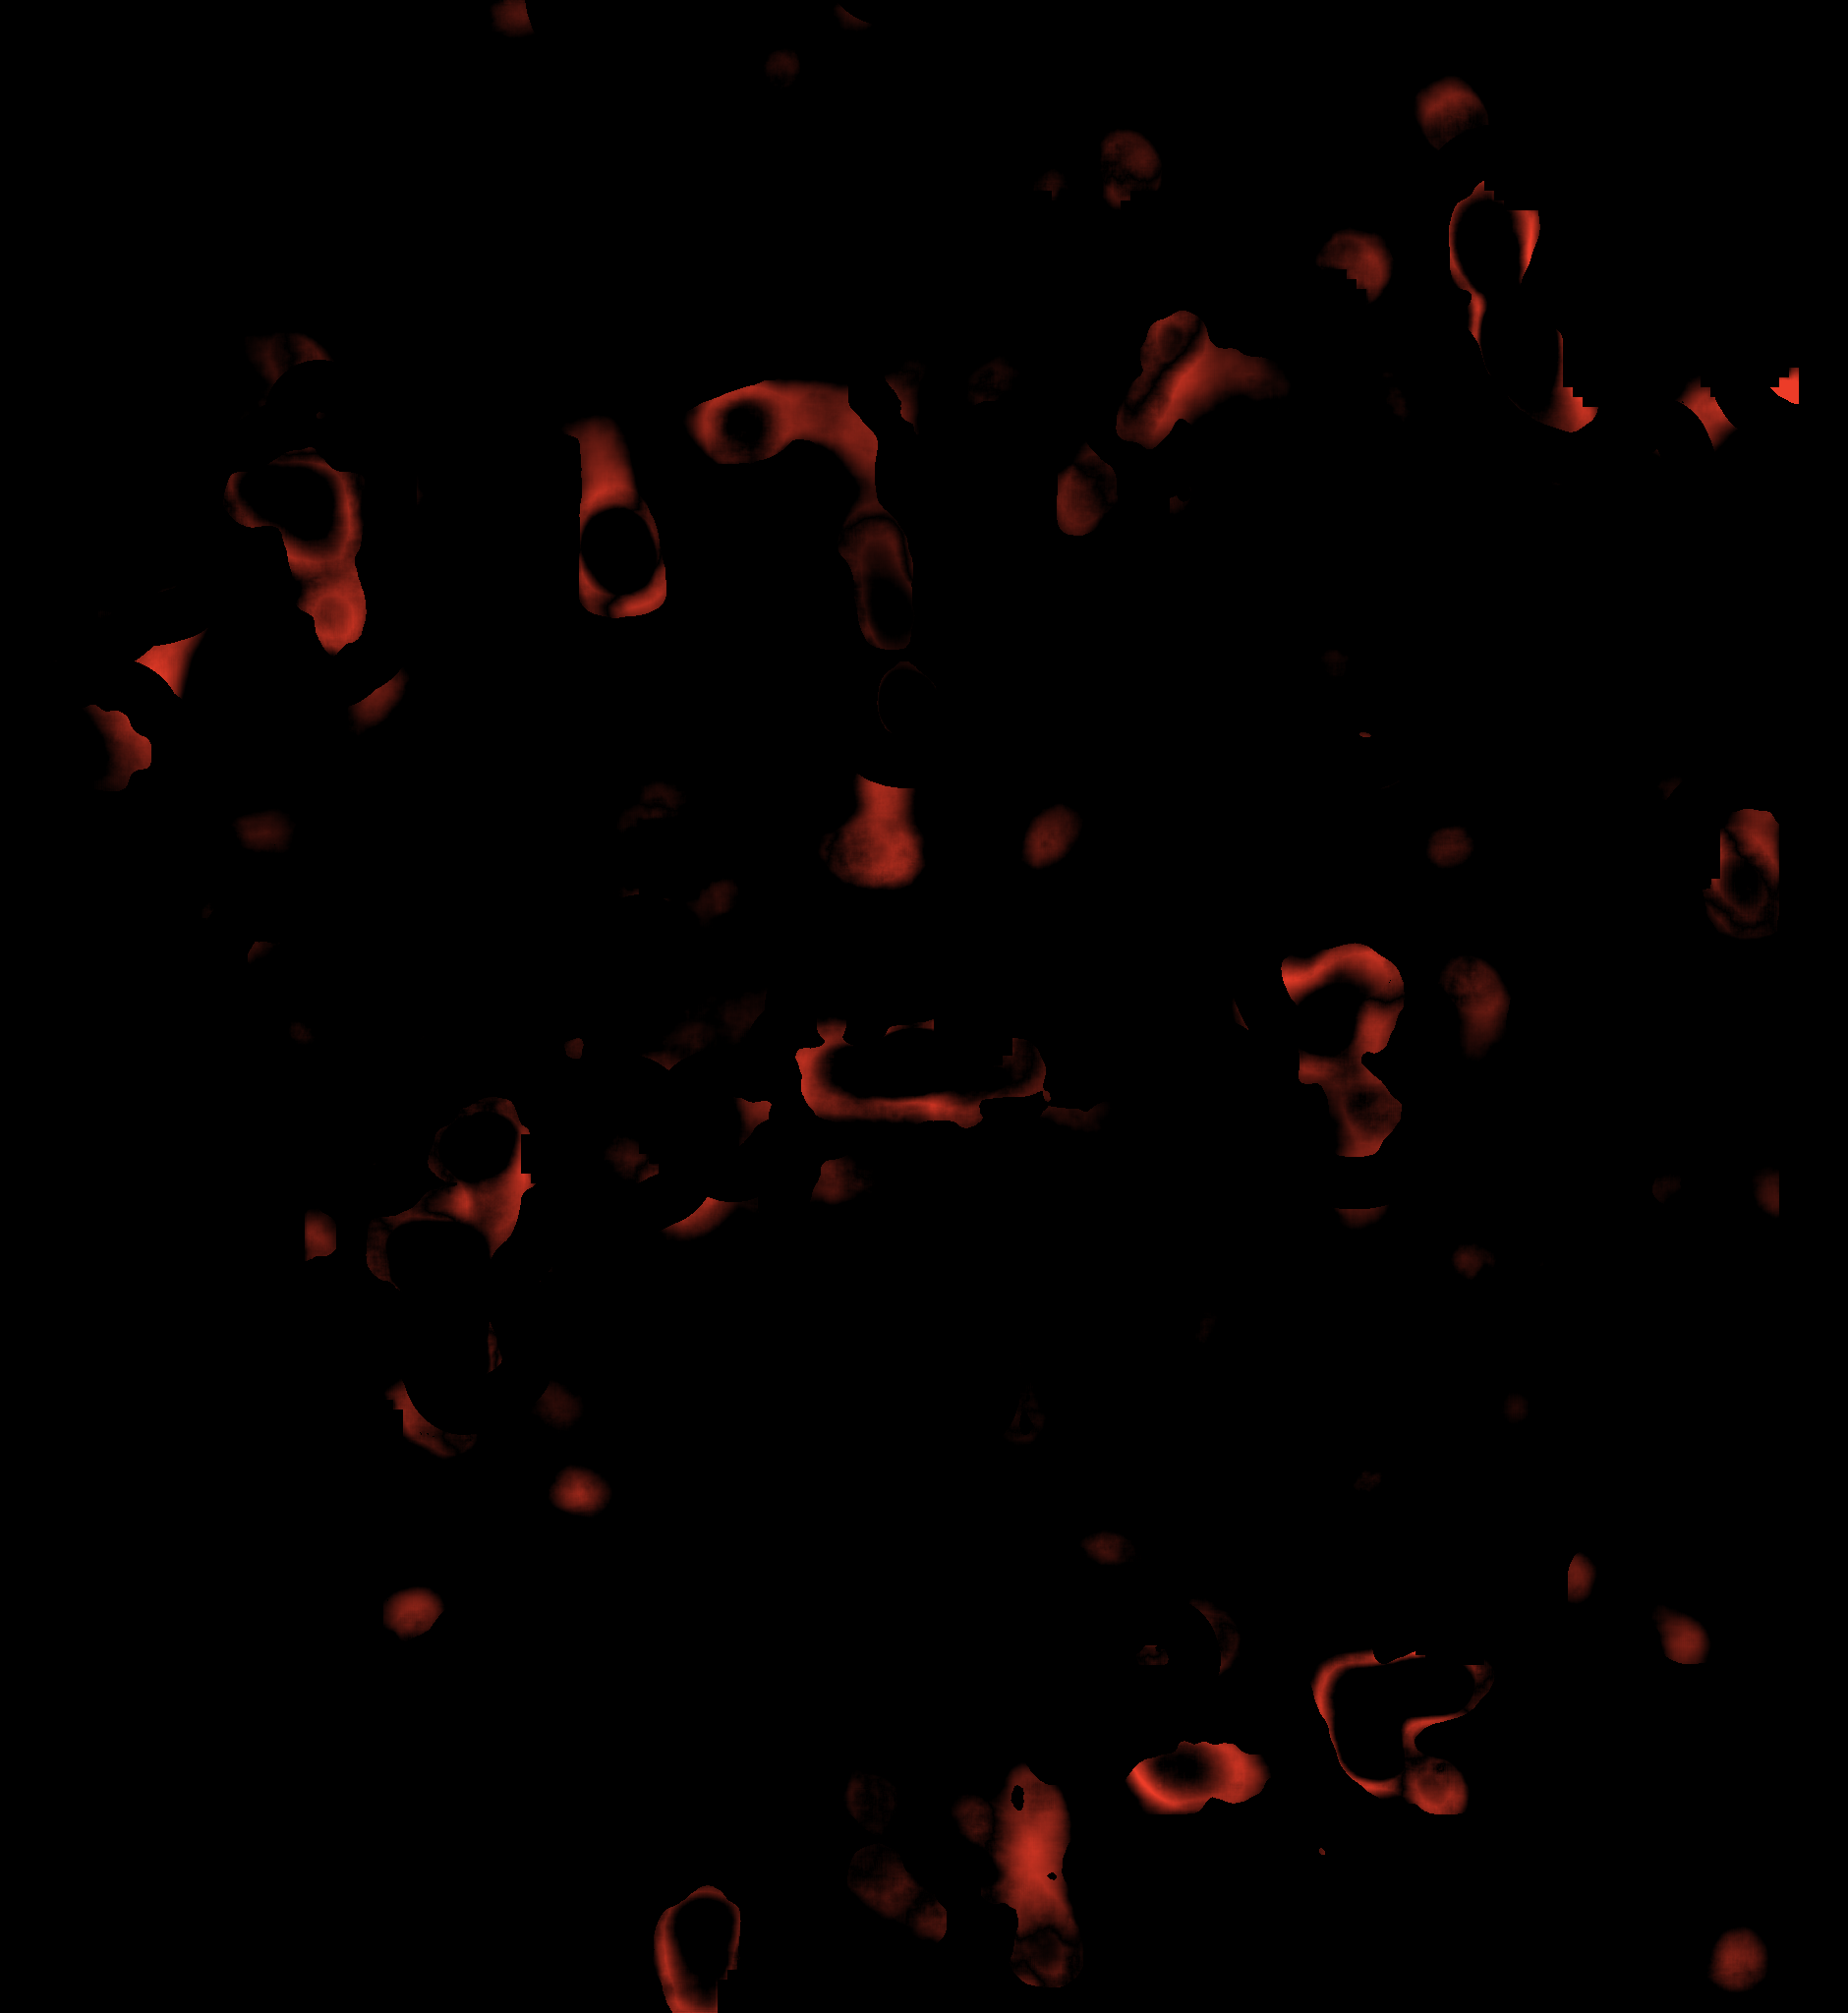
\includegraphics[width=0.29\textwidth]{../figures/m3/20250716055229_3_difference.png}
\caption{Held-out unit 0500P2$\cdot$055229. Left, Reader v3 (AUC 0.8971); centre, \MtName{} (AUC 0.8479); right, the red difference between the two maps. Each map is stretched between its own percentiles, the panels are shown at the full resolution of the file.}\label{fig:m3-20250716055229}
\end{figure*}

\begin{figure*}[!tp]
\centering
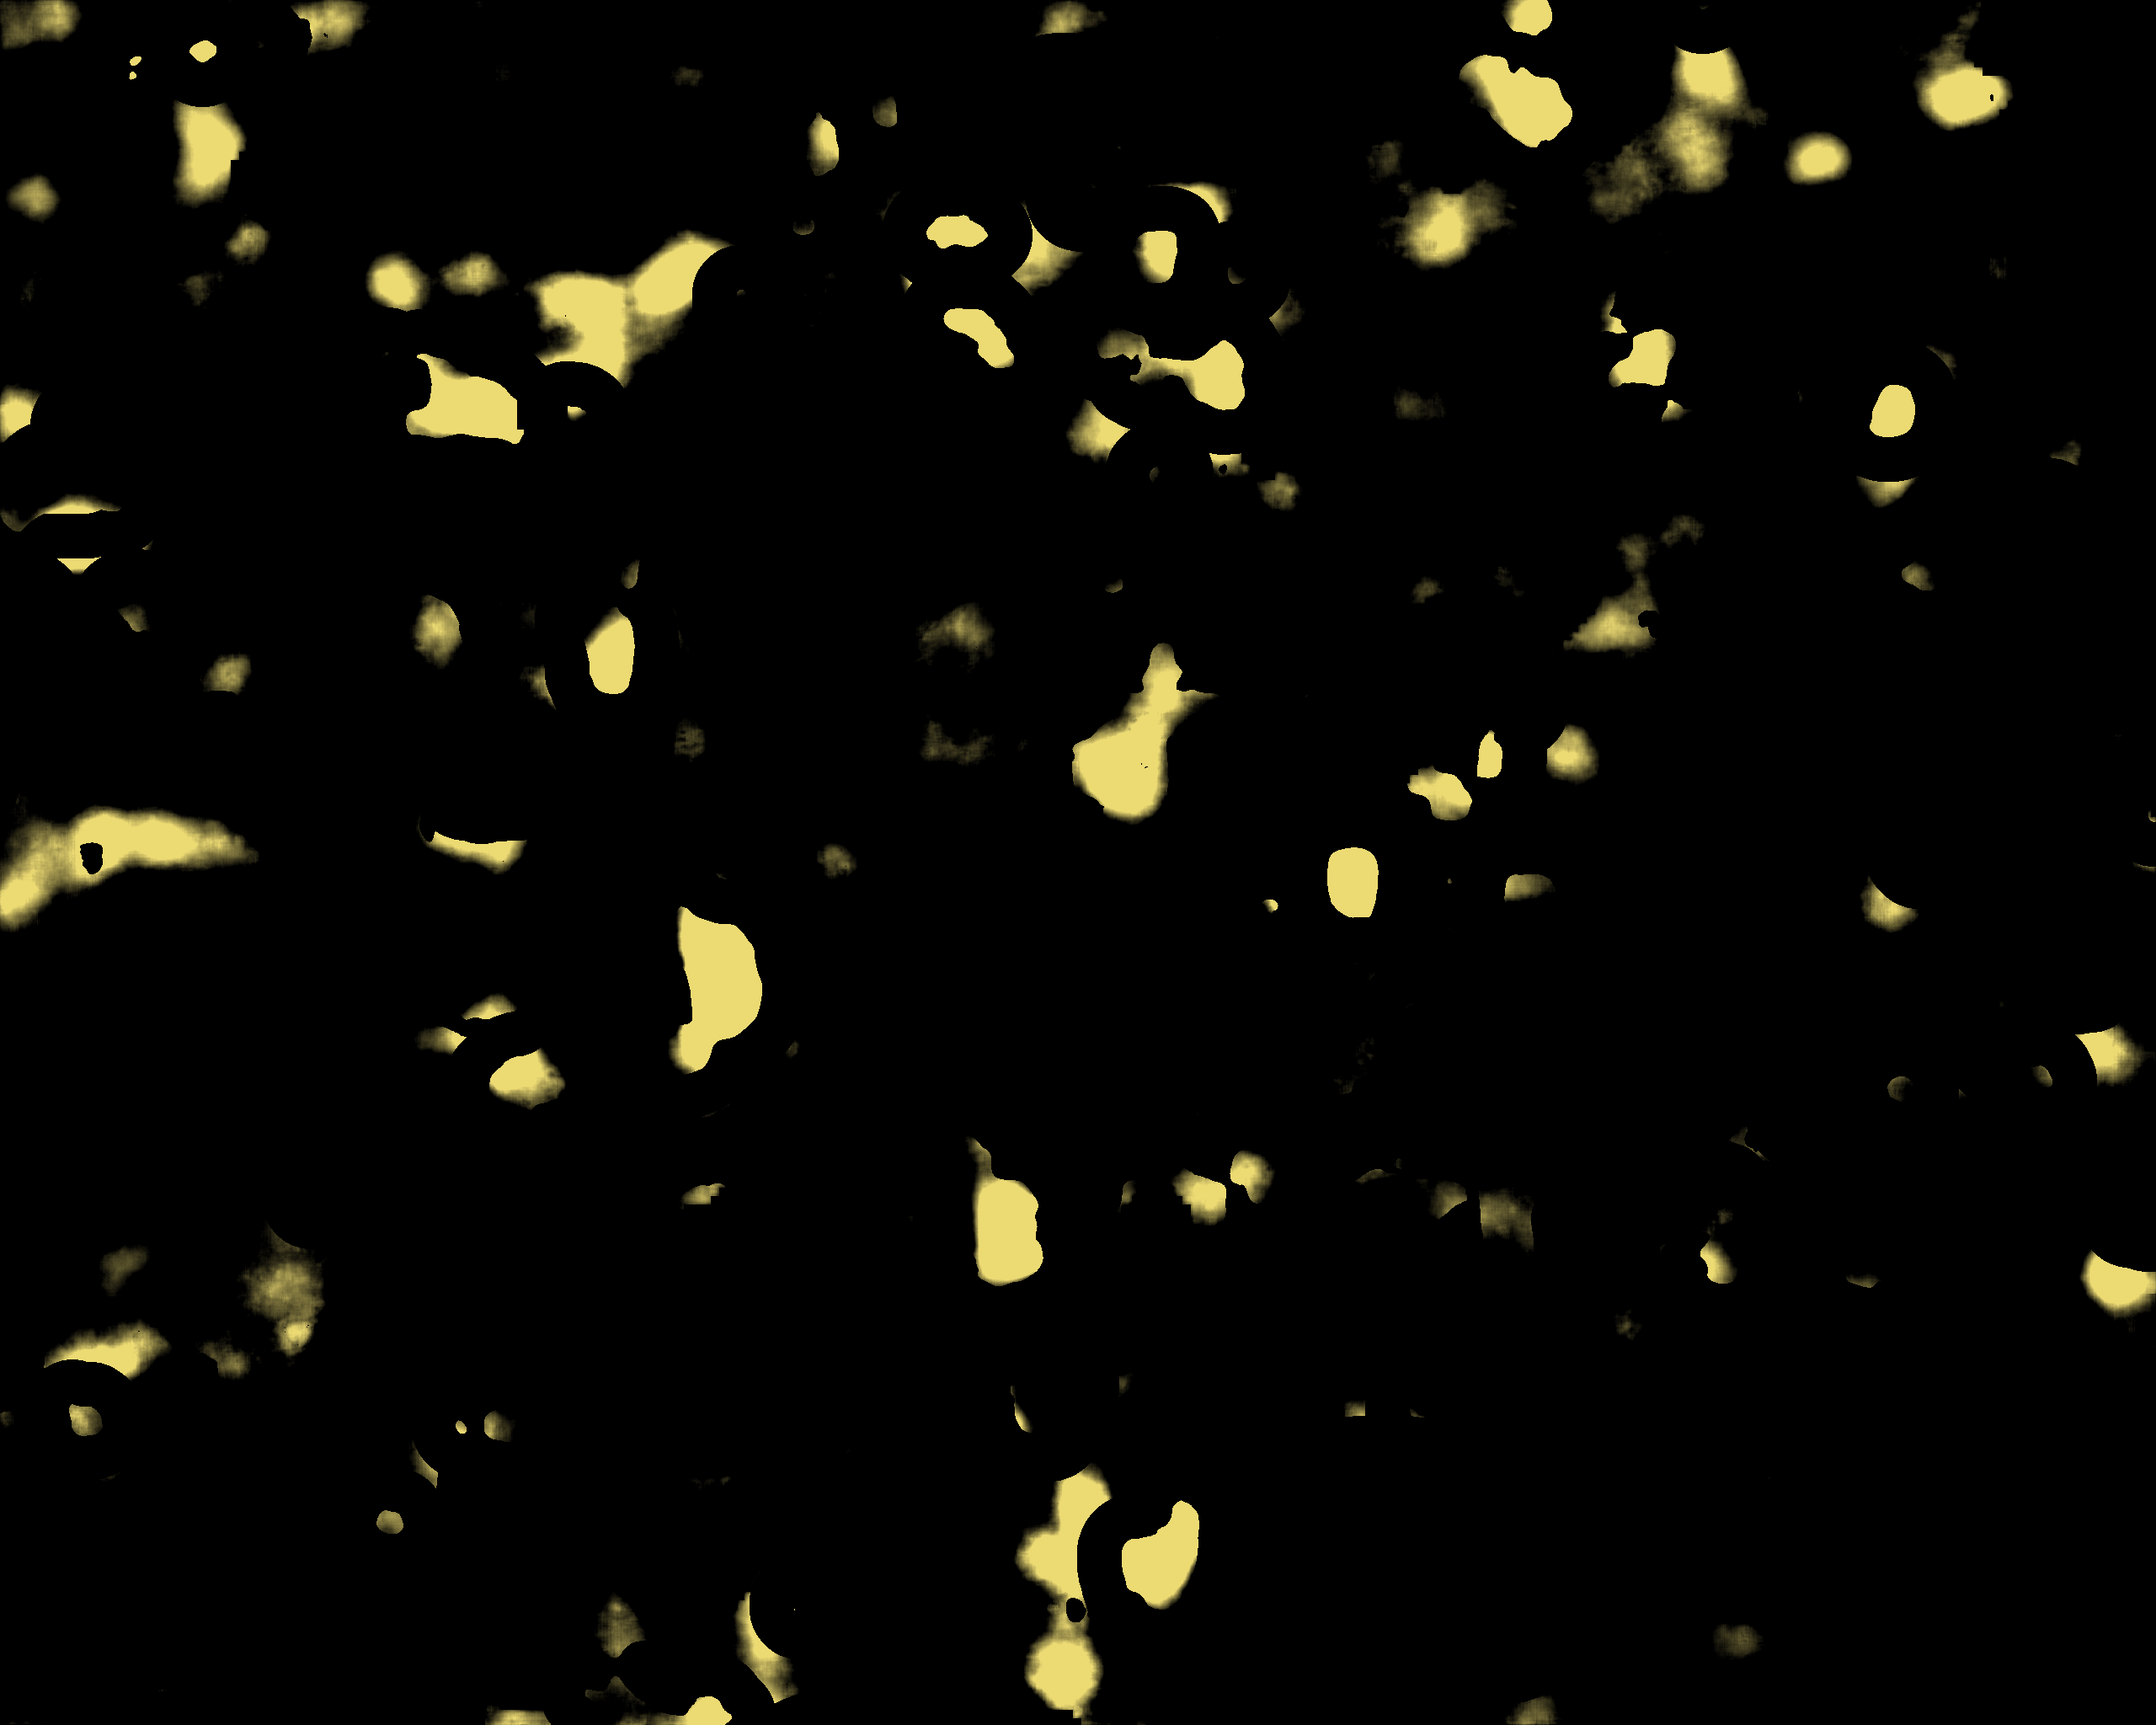
\includegraphics[width=0.29\textwidth]{../figures/m3/20250716055230_1_reader-v3.png}
\hspace{3pt}
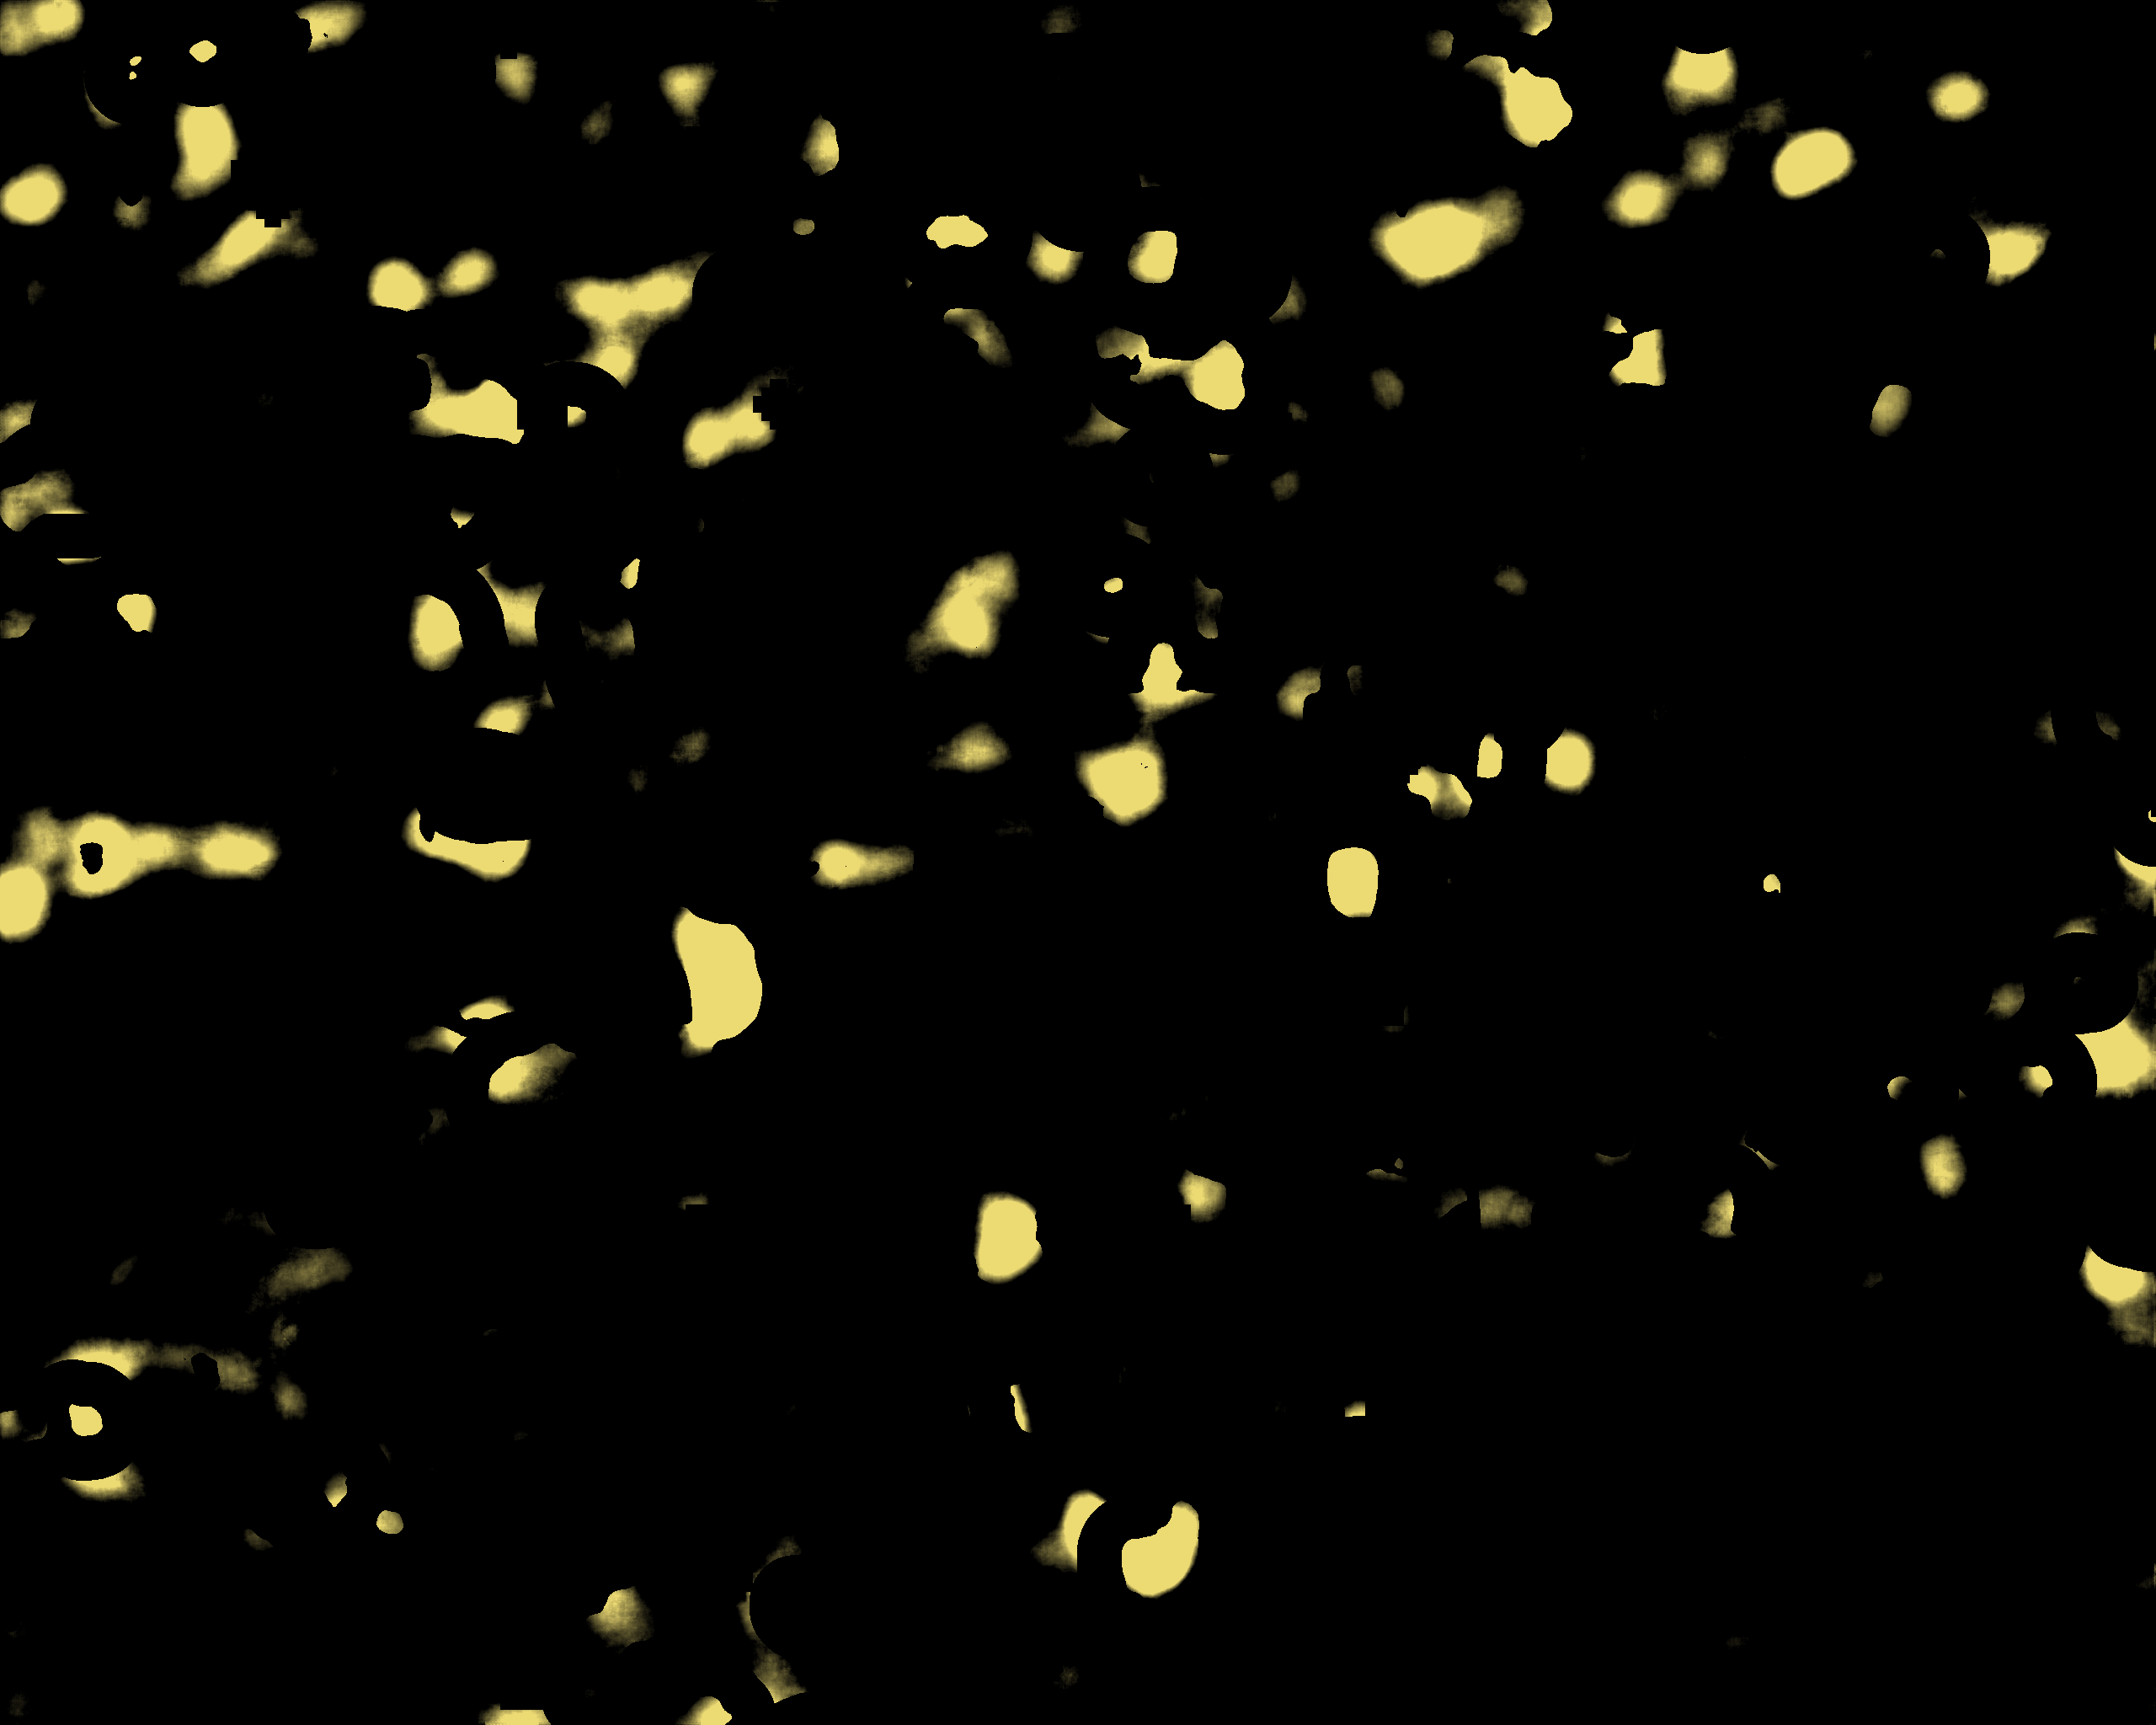
\includegraphics[width=0.29\textwidth]{../figures/m3/20250716055230_2_m3.png}
\hspace{3pt}
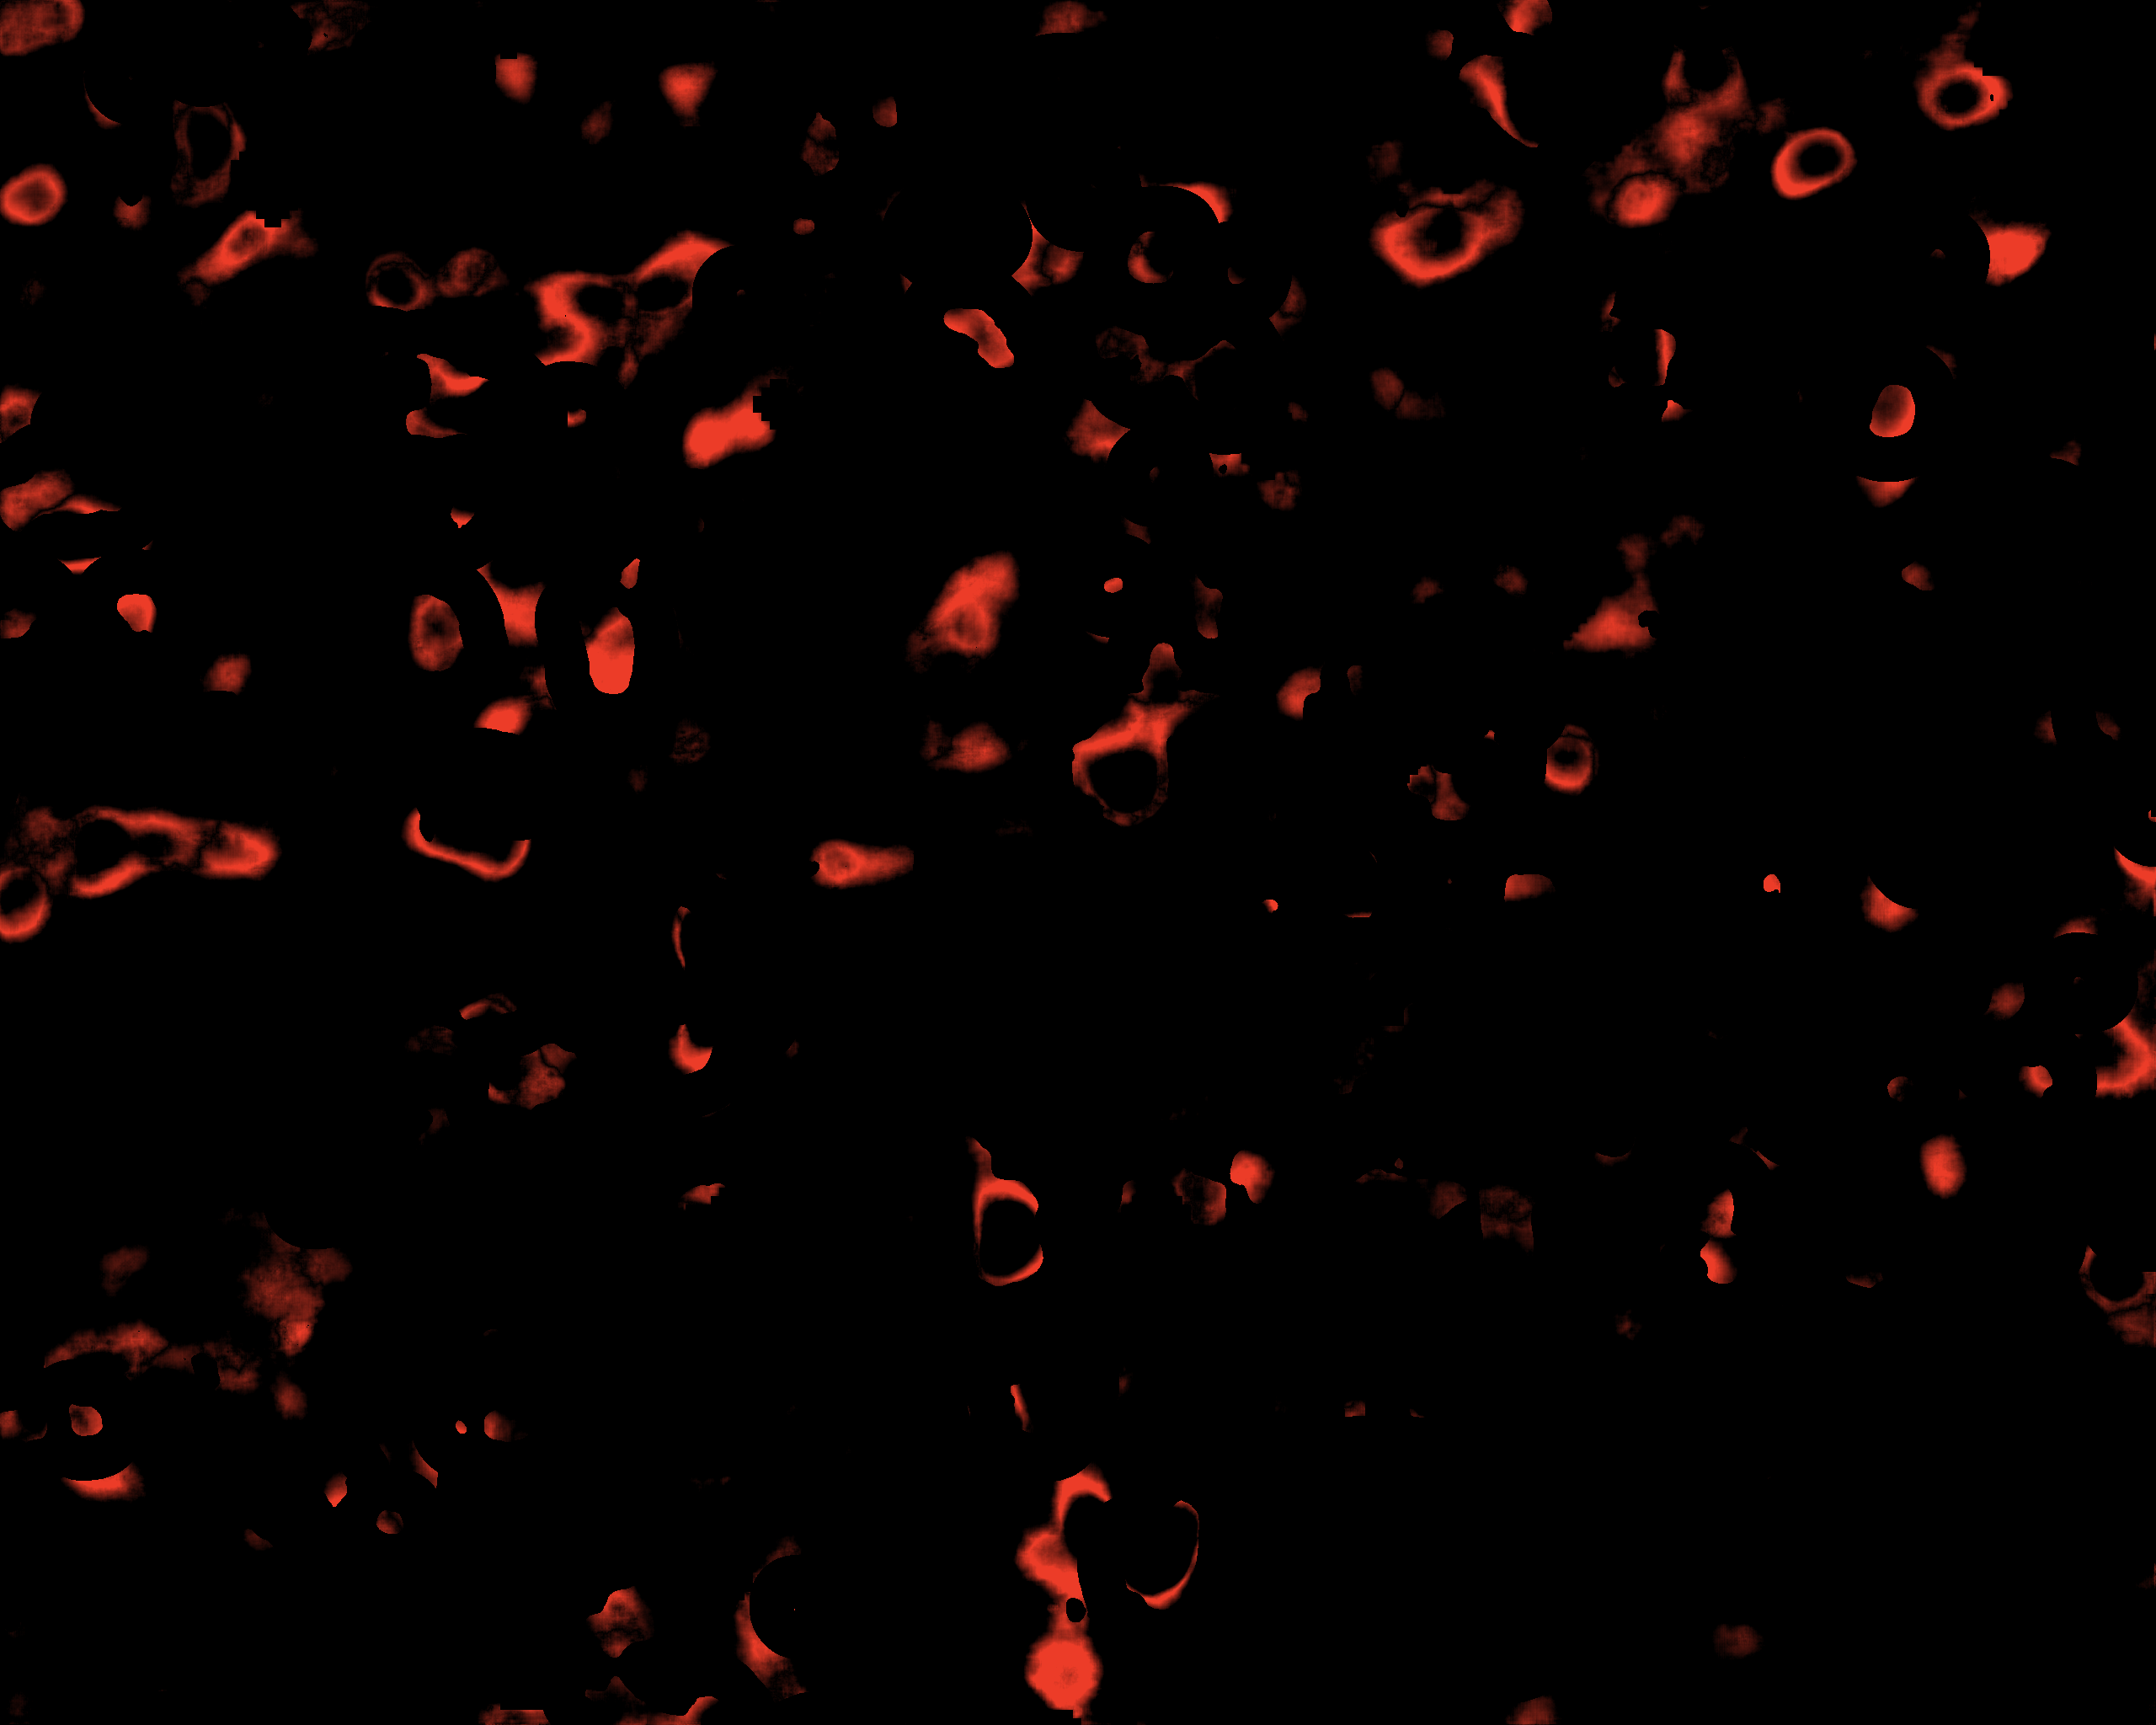
\includegraphics[width=0.29\textwidth]{../figures/m3/20250716055230_3_difference.png}
\caption{Held-out unit 0500P2$\cdot$055230. Left, Reader v3 (AUC 0.7881); centre, \MtName{} (AUC 0.7778); right, the red difference between the two maps. Each map is stretched between its own percentiles, the panels are shown at the full resolution of the file.}\label{fig:m3-20250716055230}
\end{figure*}

\begin{figure*}[!tp]
\centering
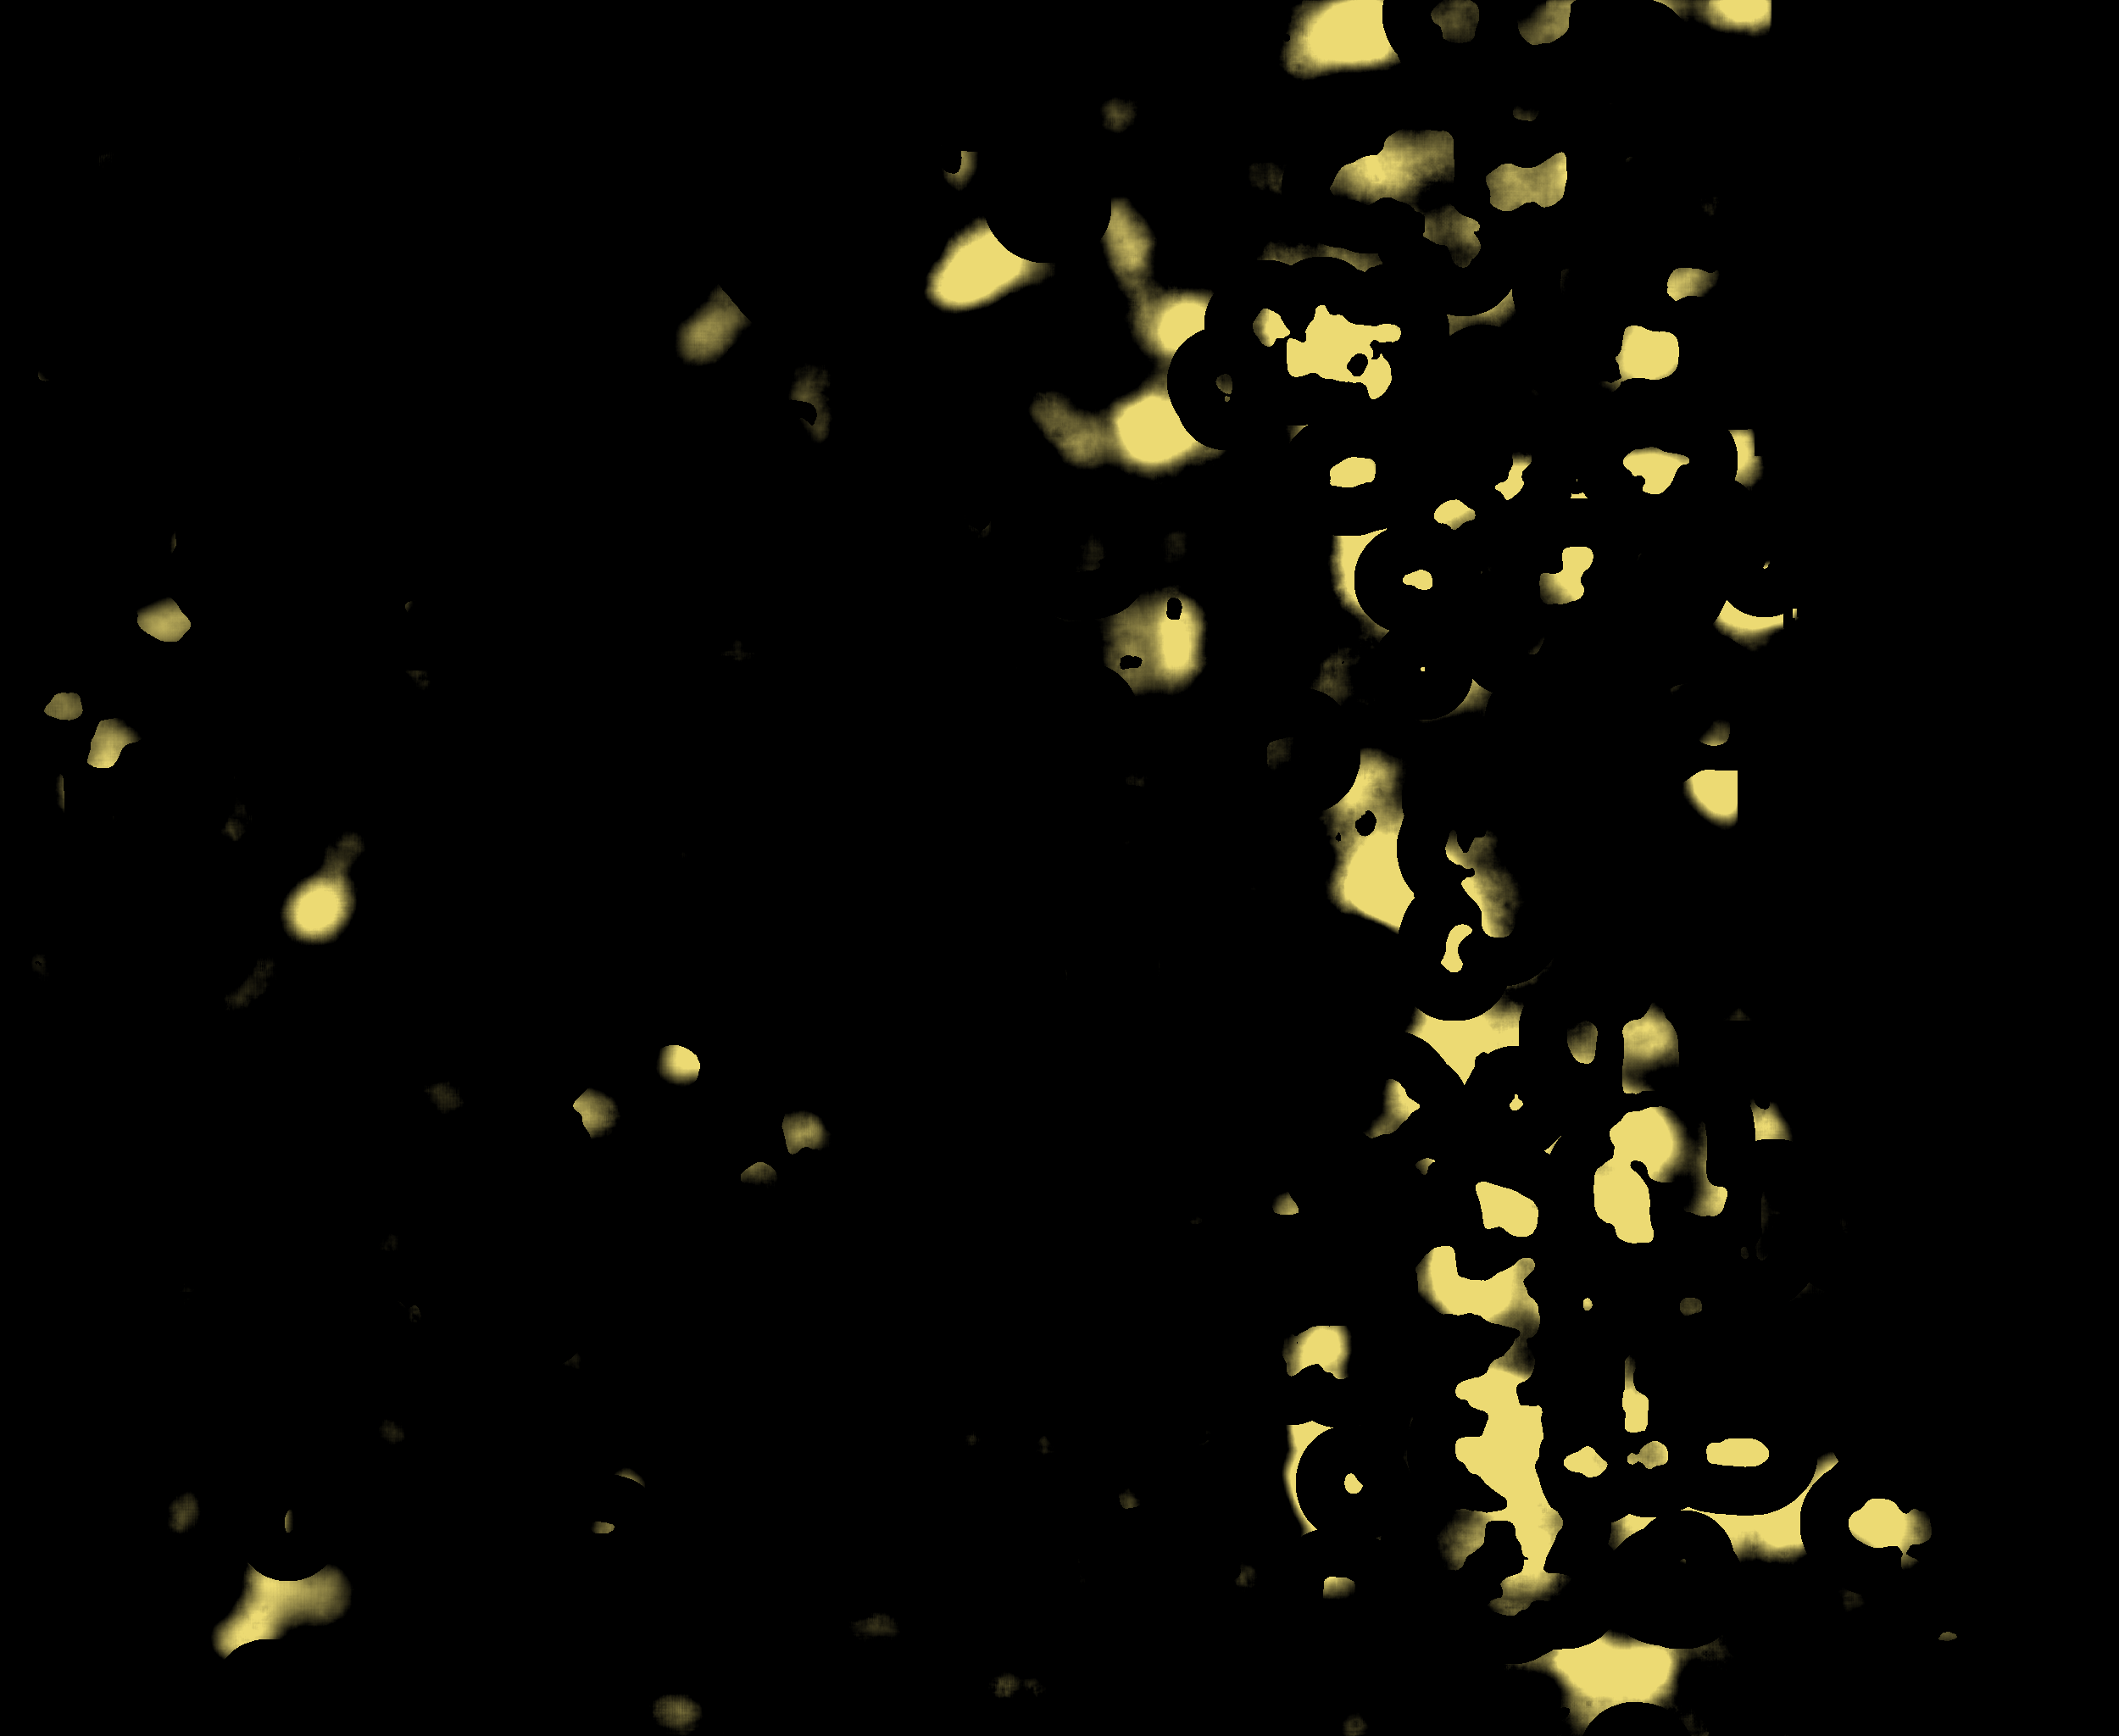
\includegraphics[width=0.29\textwidth]{../figures/m3/20250904233748-0_b2_1_reader-v3.png}
\hspace{3pt}
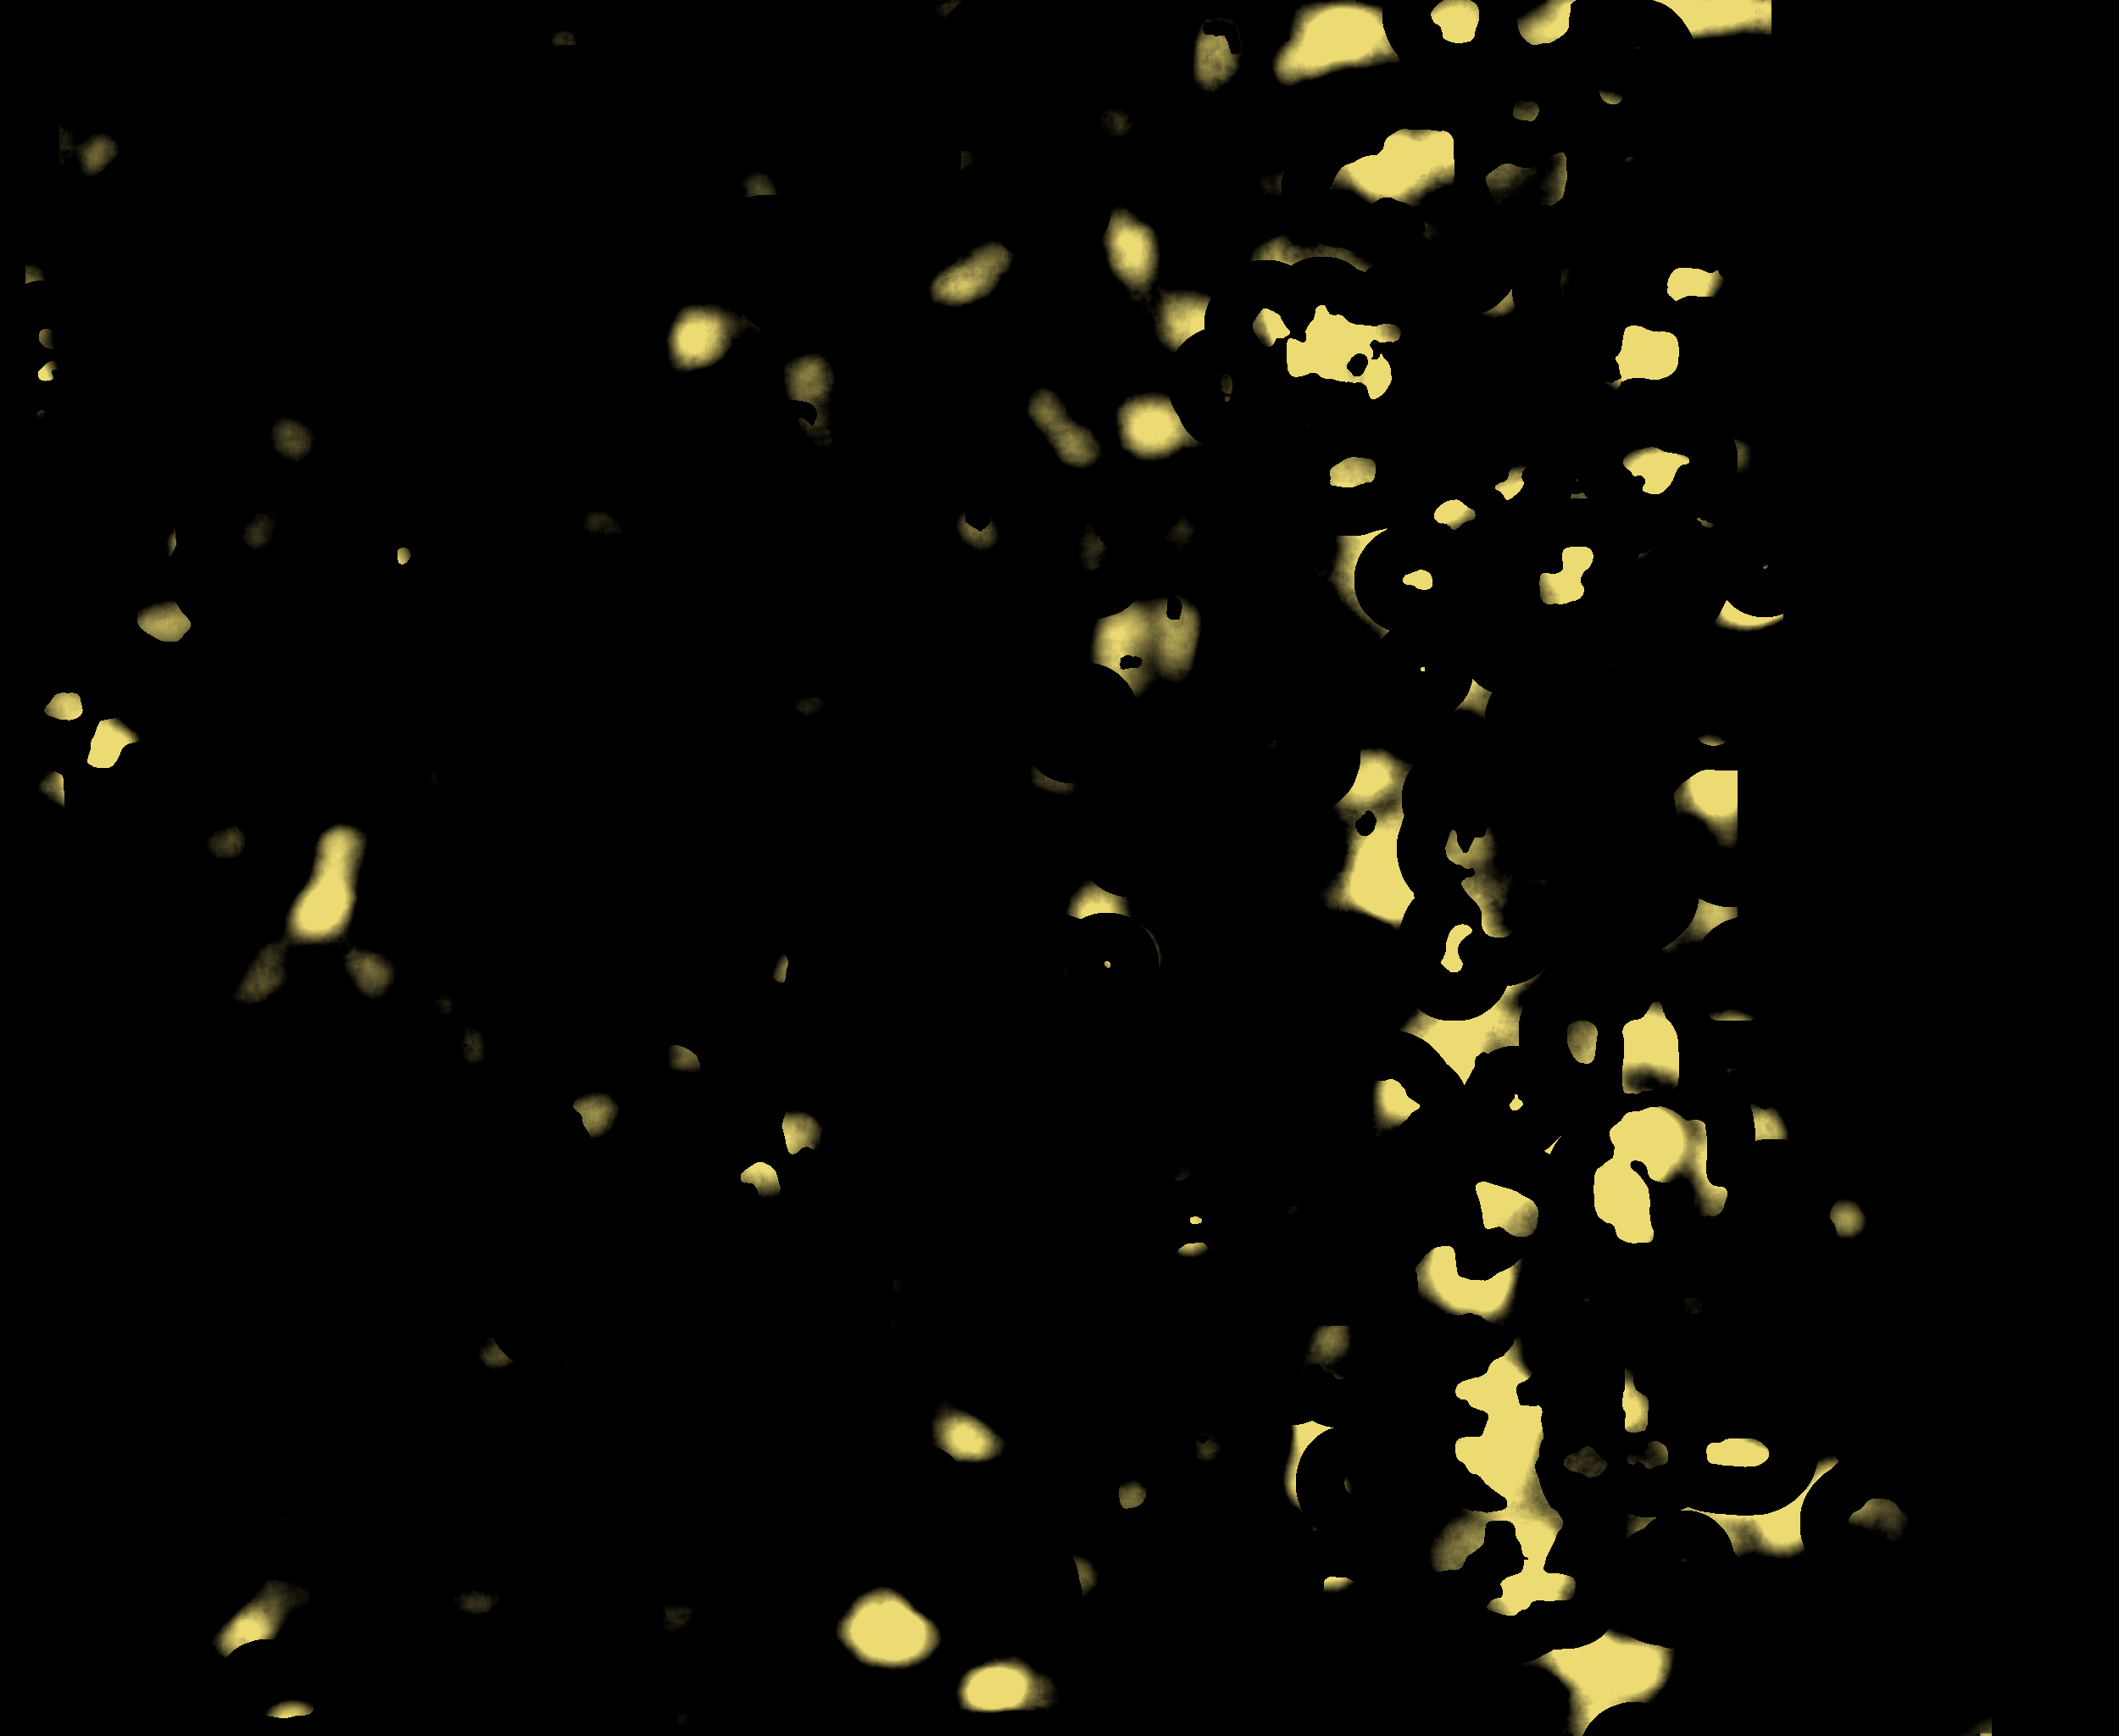
\includegraphics[width=0.29\textwidth]{../figures/m3/20250904233748-0_b2_2_m3.png}
\hspace{3pt}
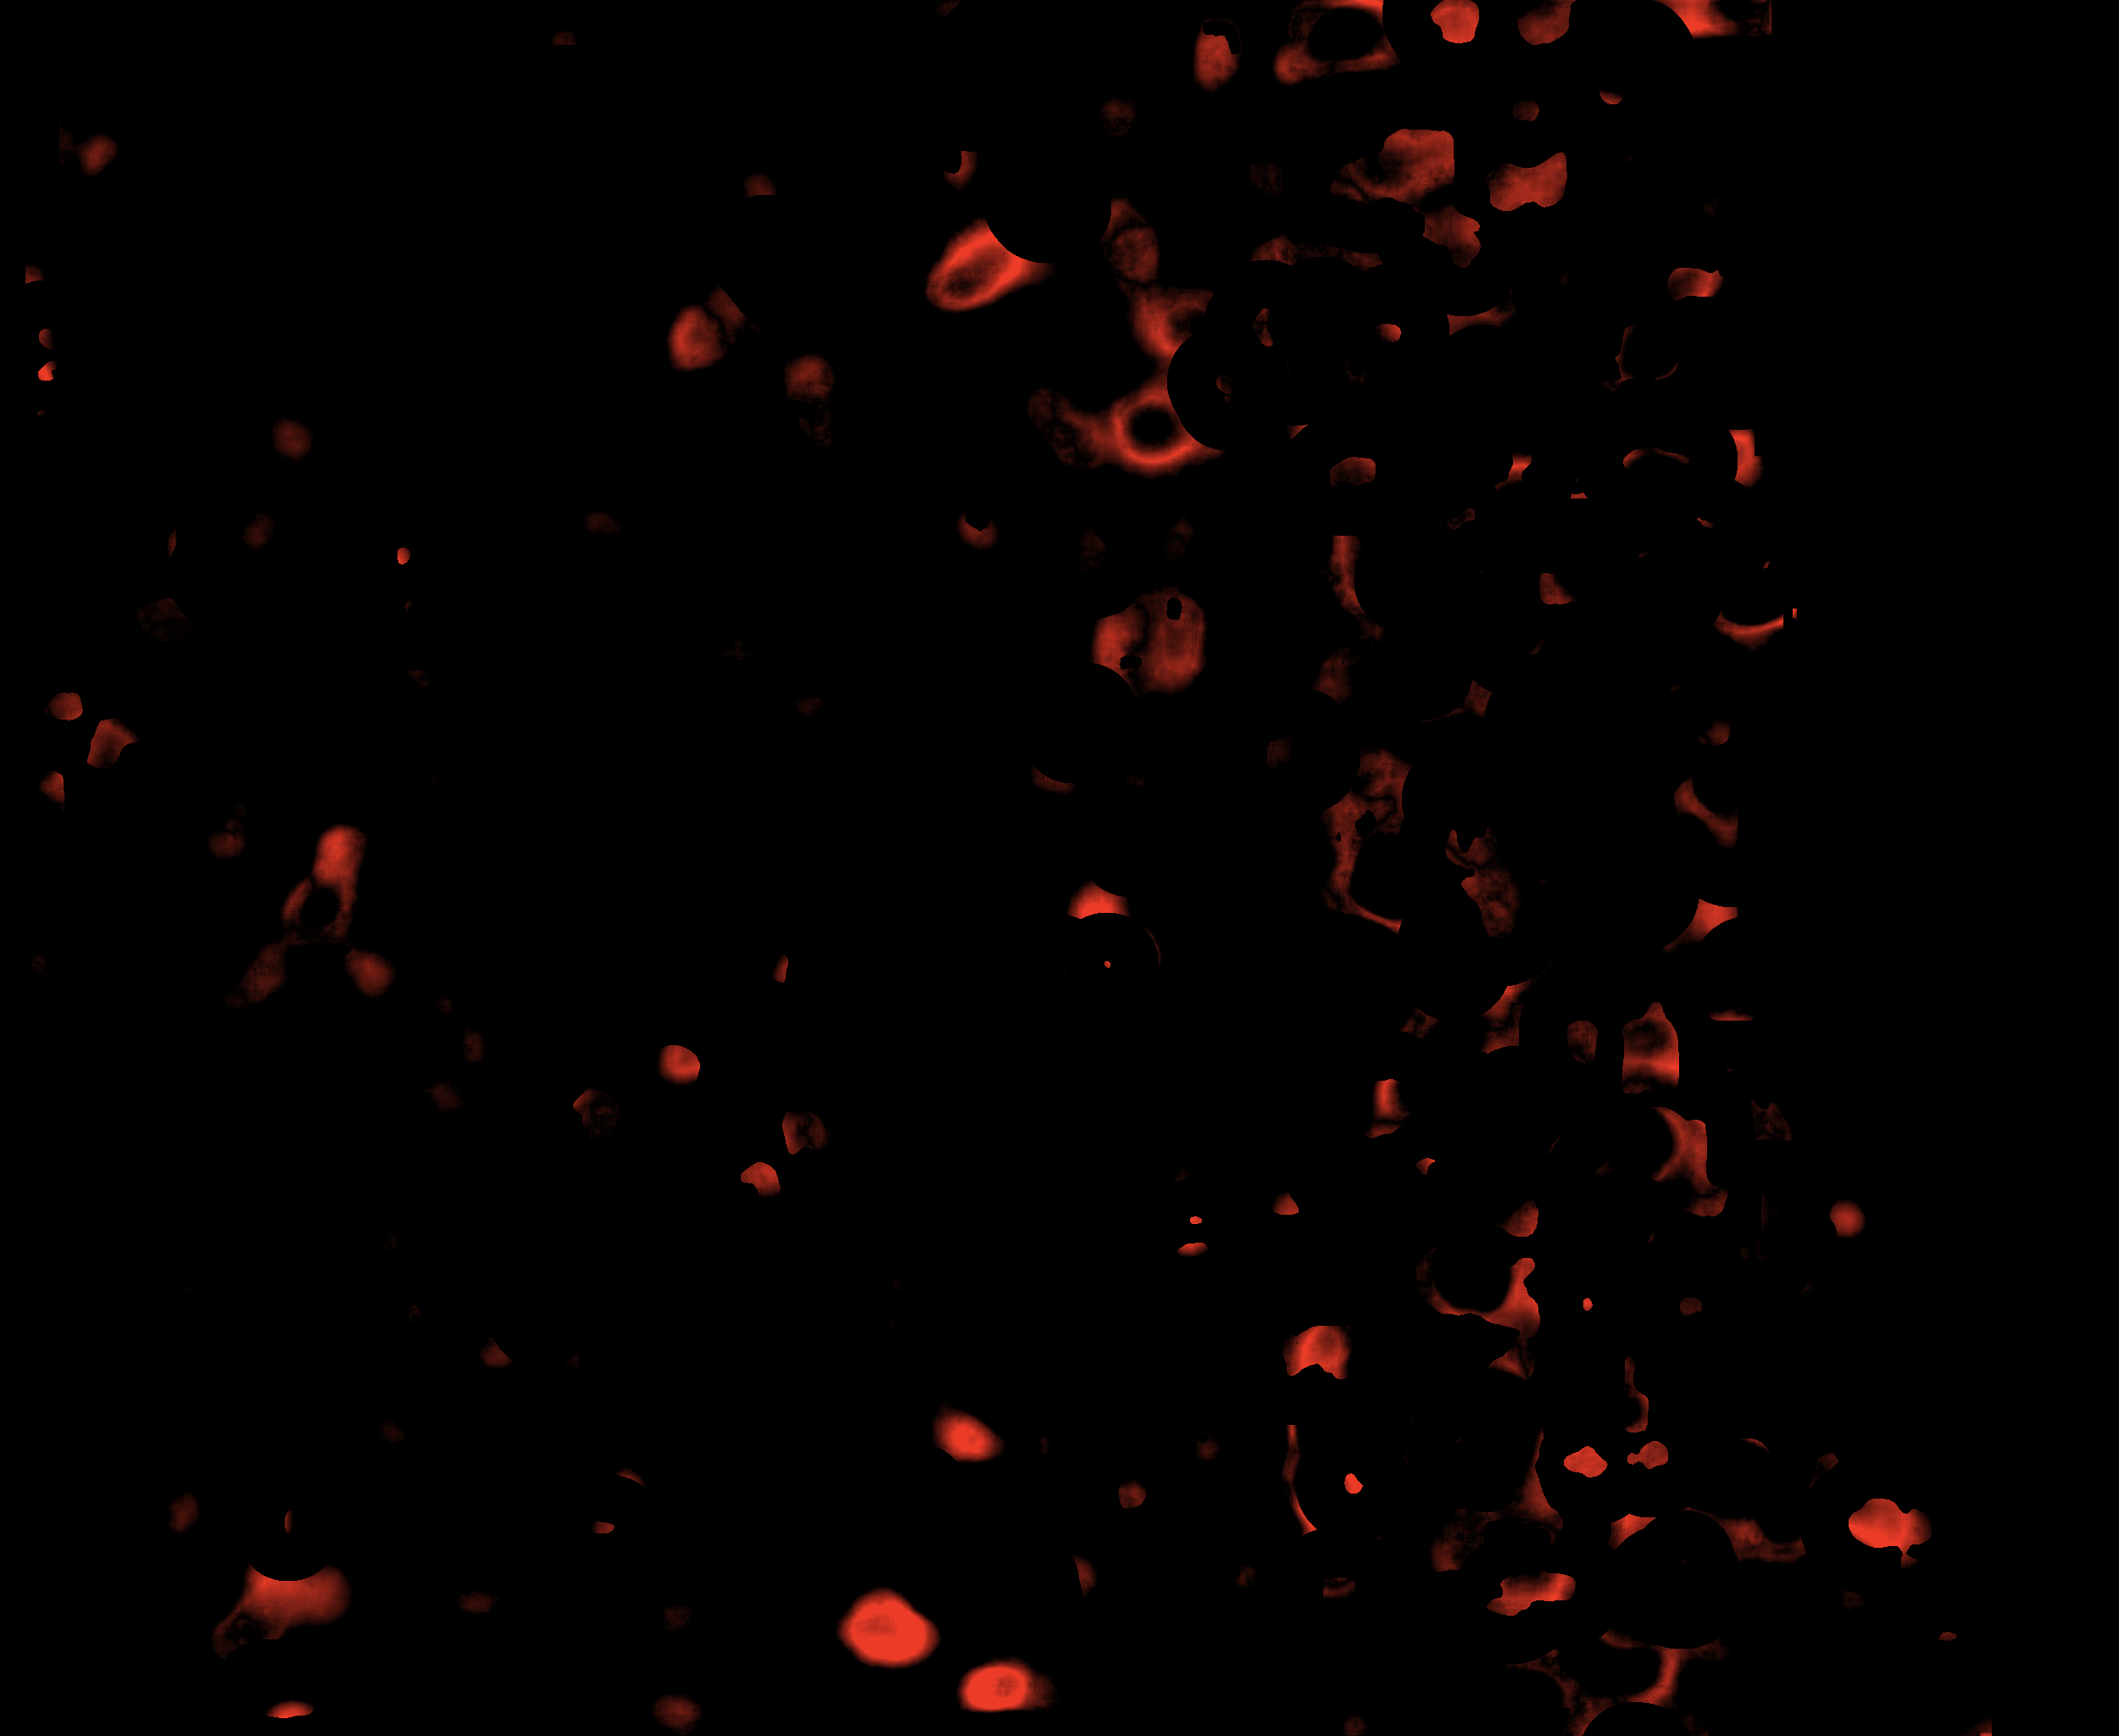
\includegraphics[width=0.29\textwidth]{../figures/m3/20250904233748-0_b2_3_difference.png}
\caption{Held-out unit 0343P$\cdot$233748-0. Left, Reader v3 (AUC 0.8340); centre, \MtName{} (AUC 0.8377); right, the red difference between the two maps. Each map is stretched between its own percentiles, the panels are shown at the full resolution of the file.}\label{fig:m3-20250904233748-0b2}
\end{figure*}

\begin{figure*}[!tp]
\centering
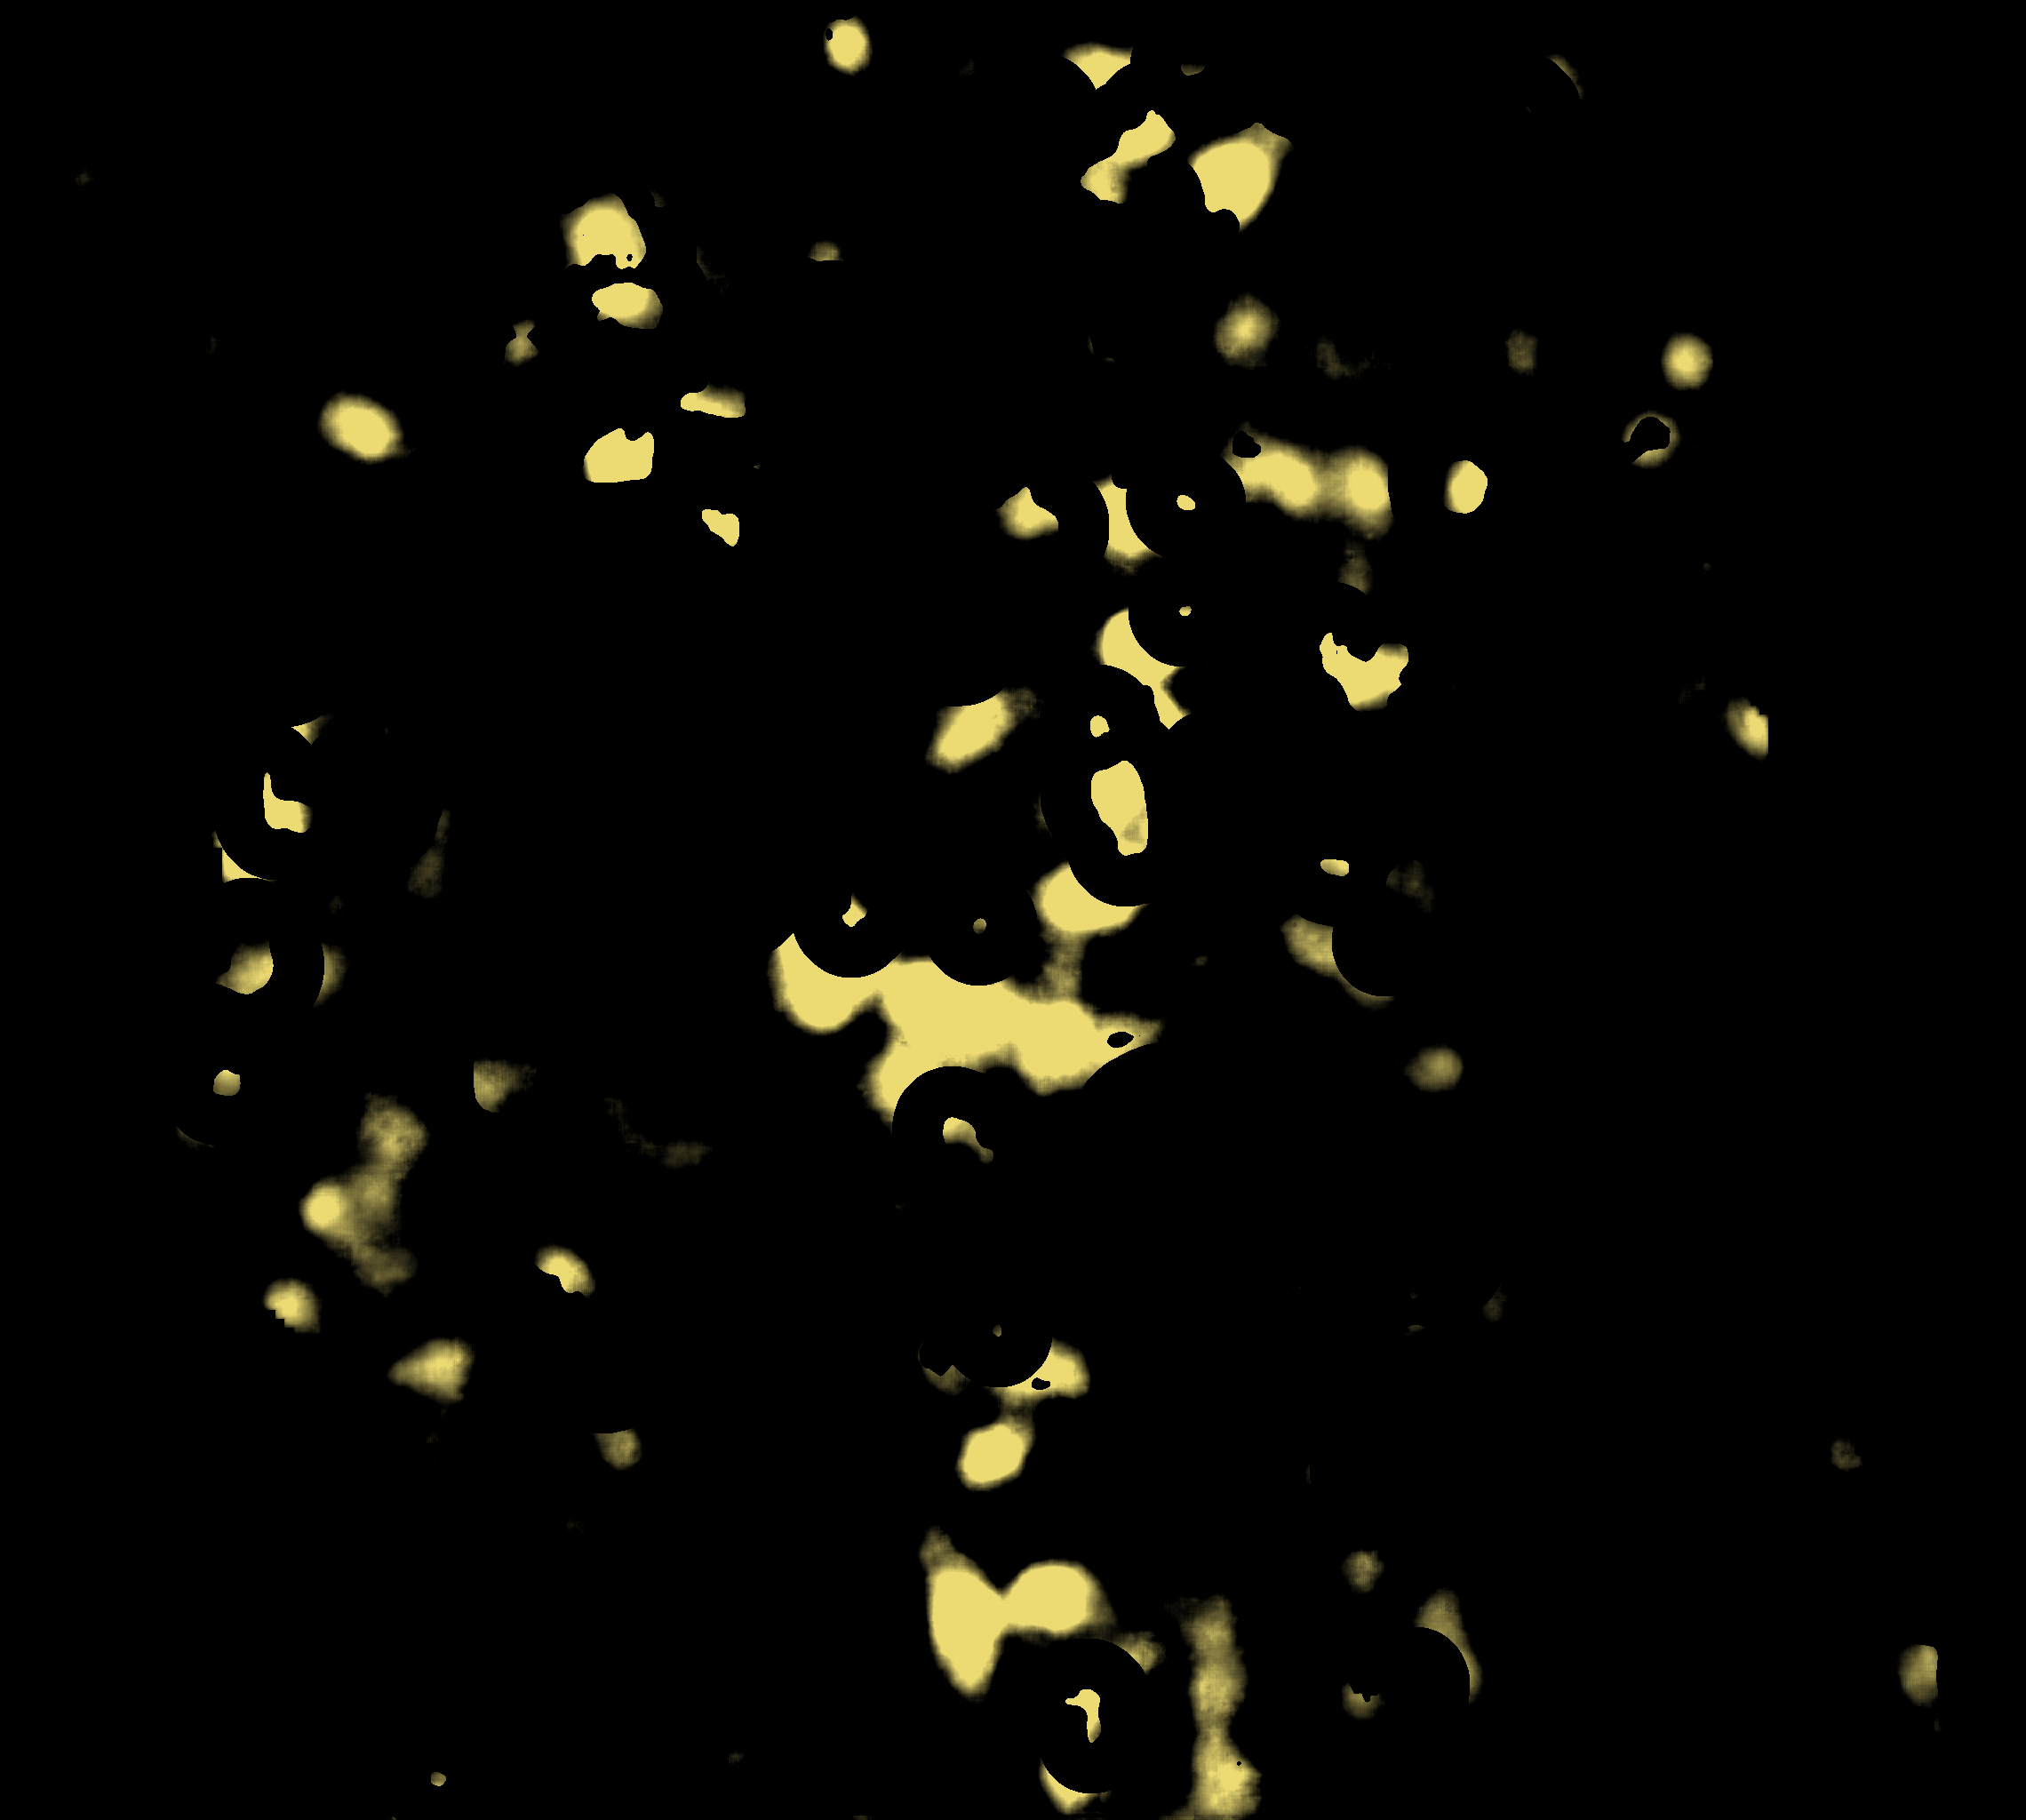
\includegraphics[width=0.29\textwidth]{../figures/m3/20250905172054-1_b2_1_reader-v3.png}
\hspace{3pt}
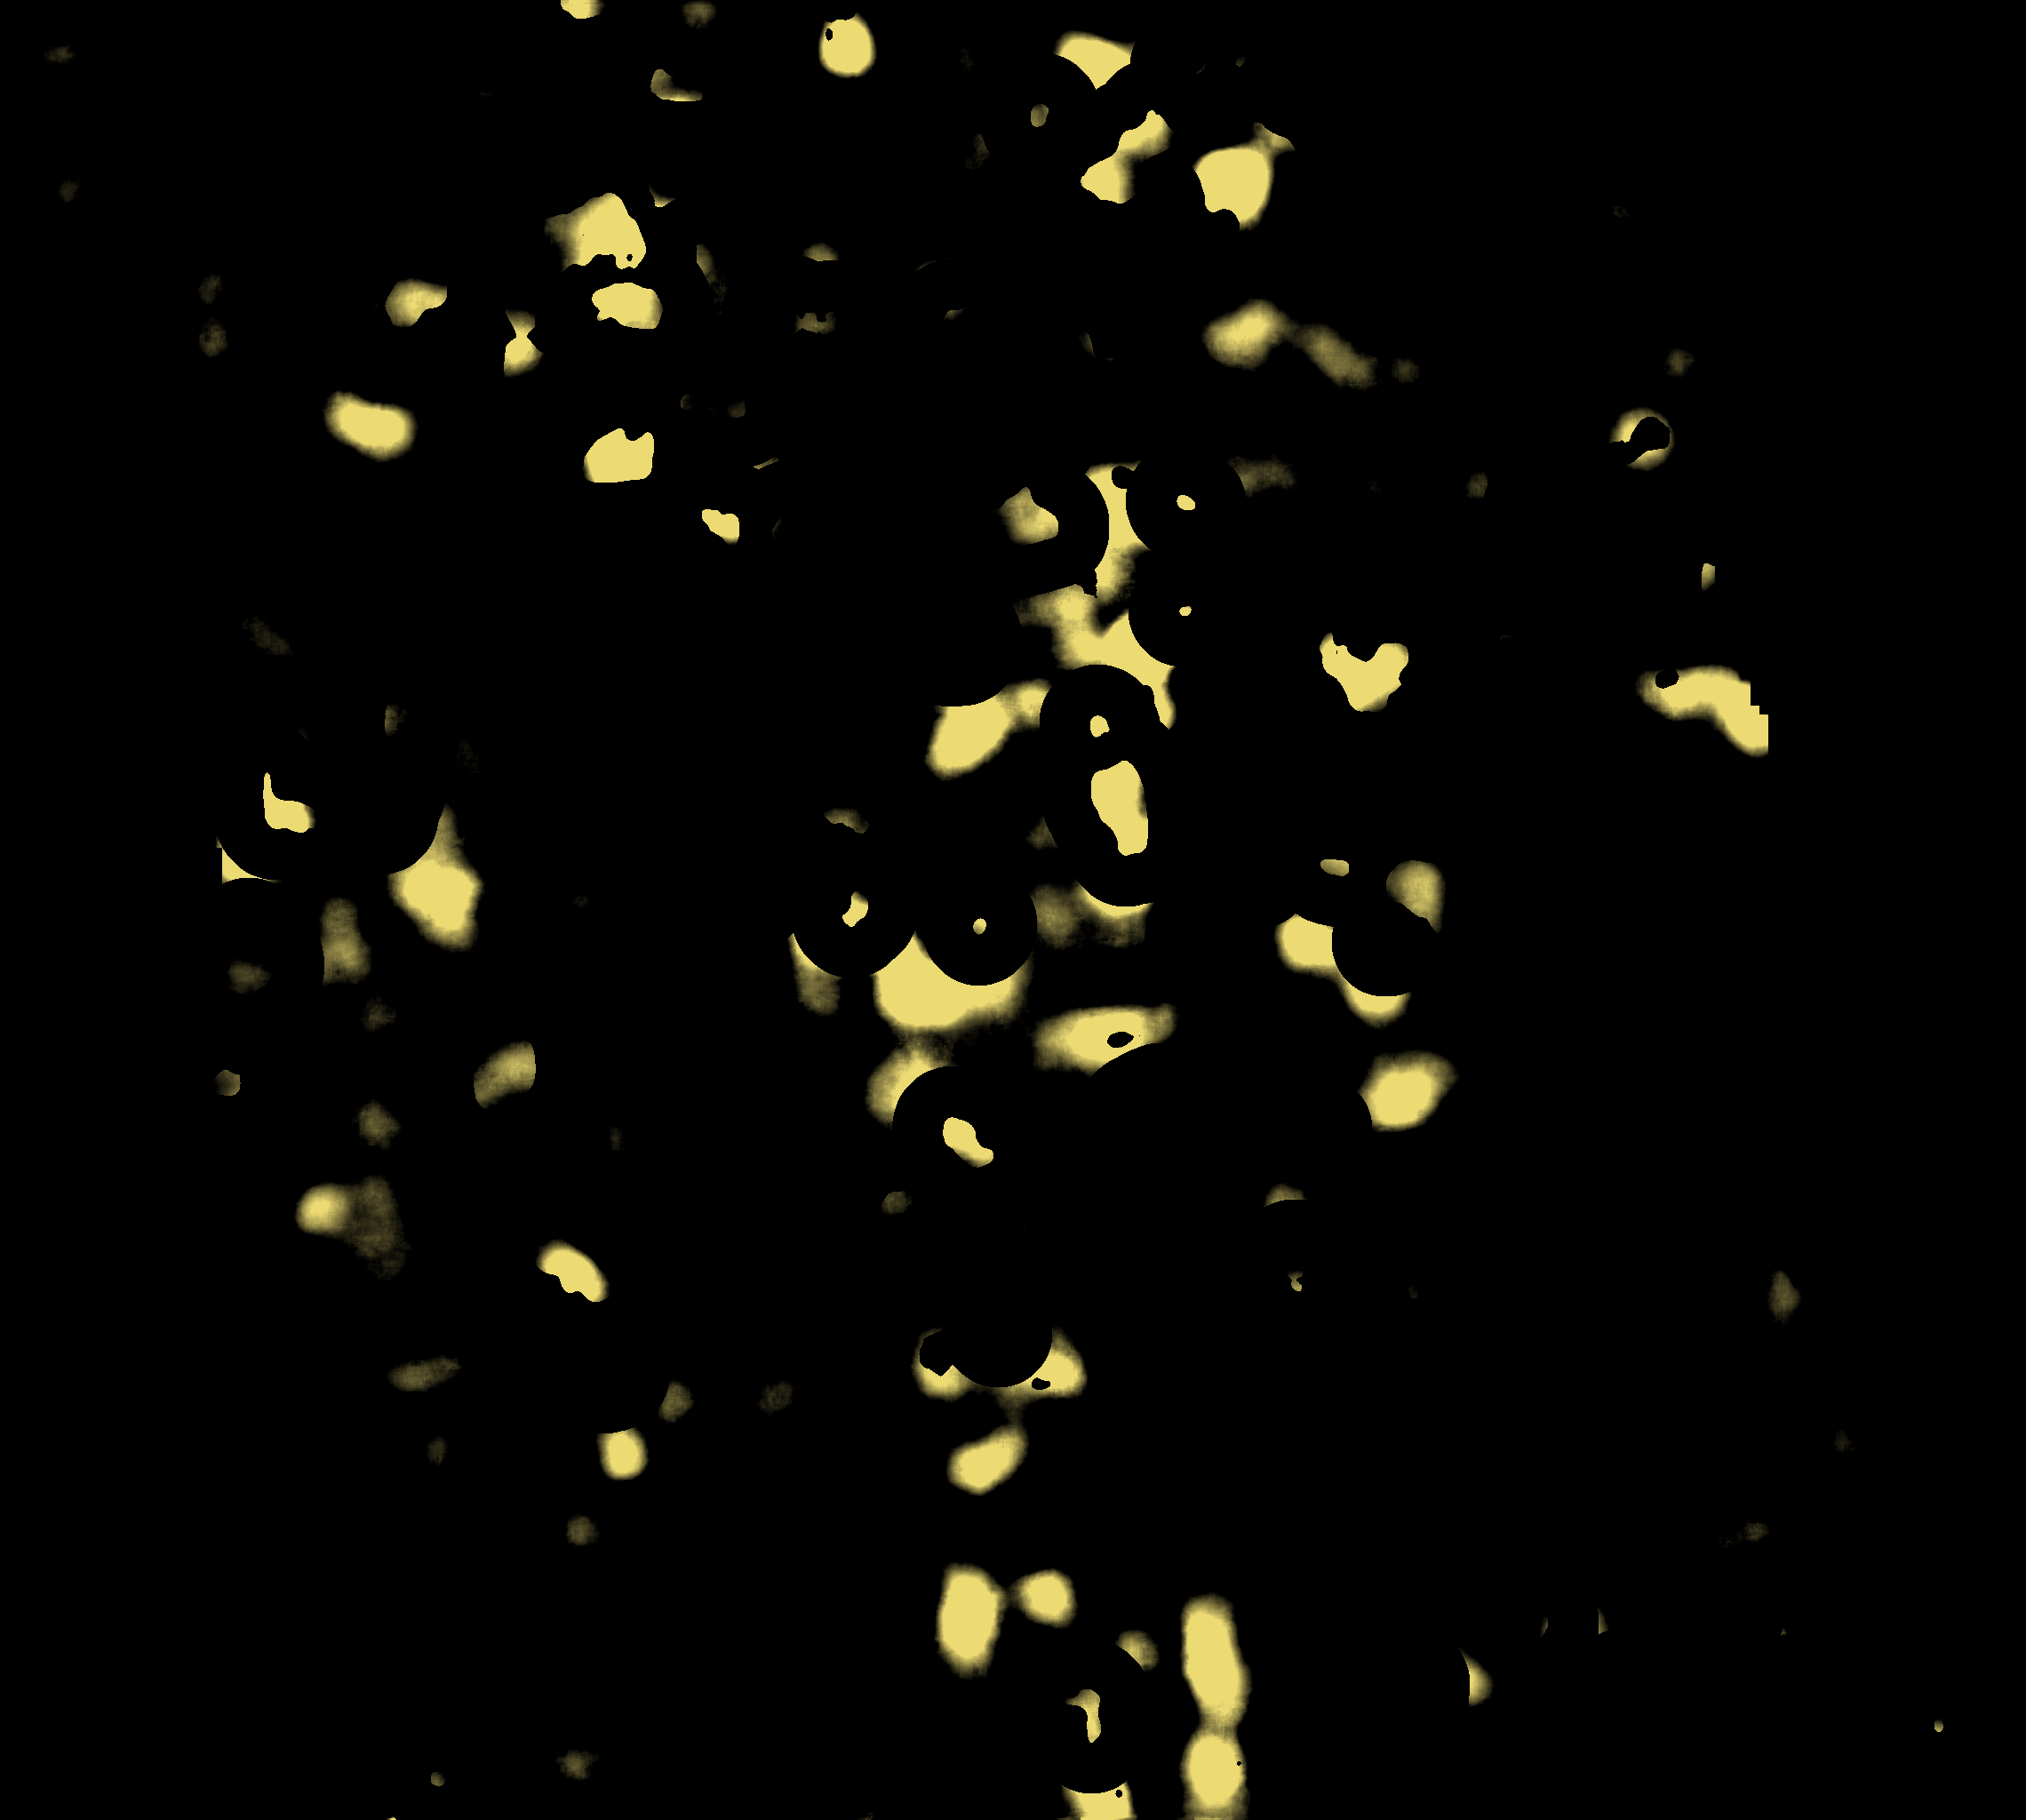
\includegraphics[width=0.29\textwidth]{../figures/m3/20250905172054-1_b2_2_m3.png}
\hspace{3pt}
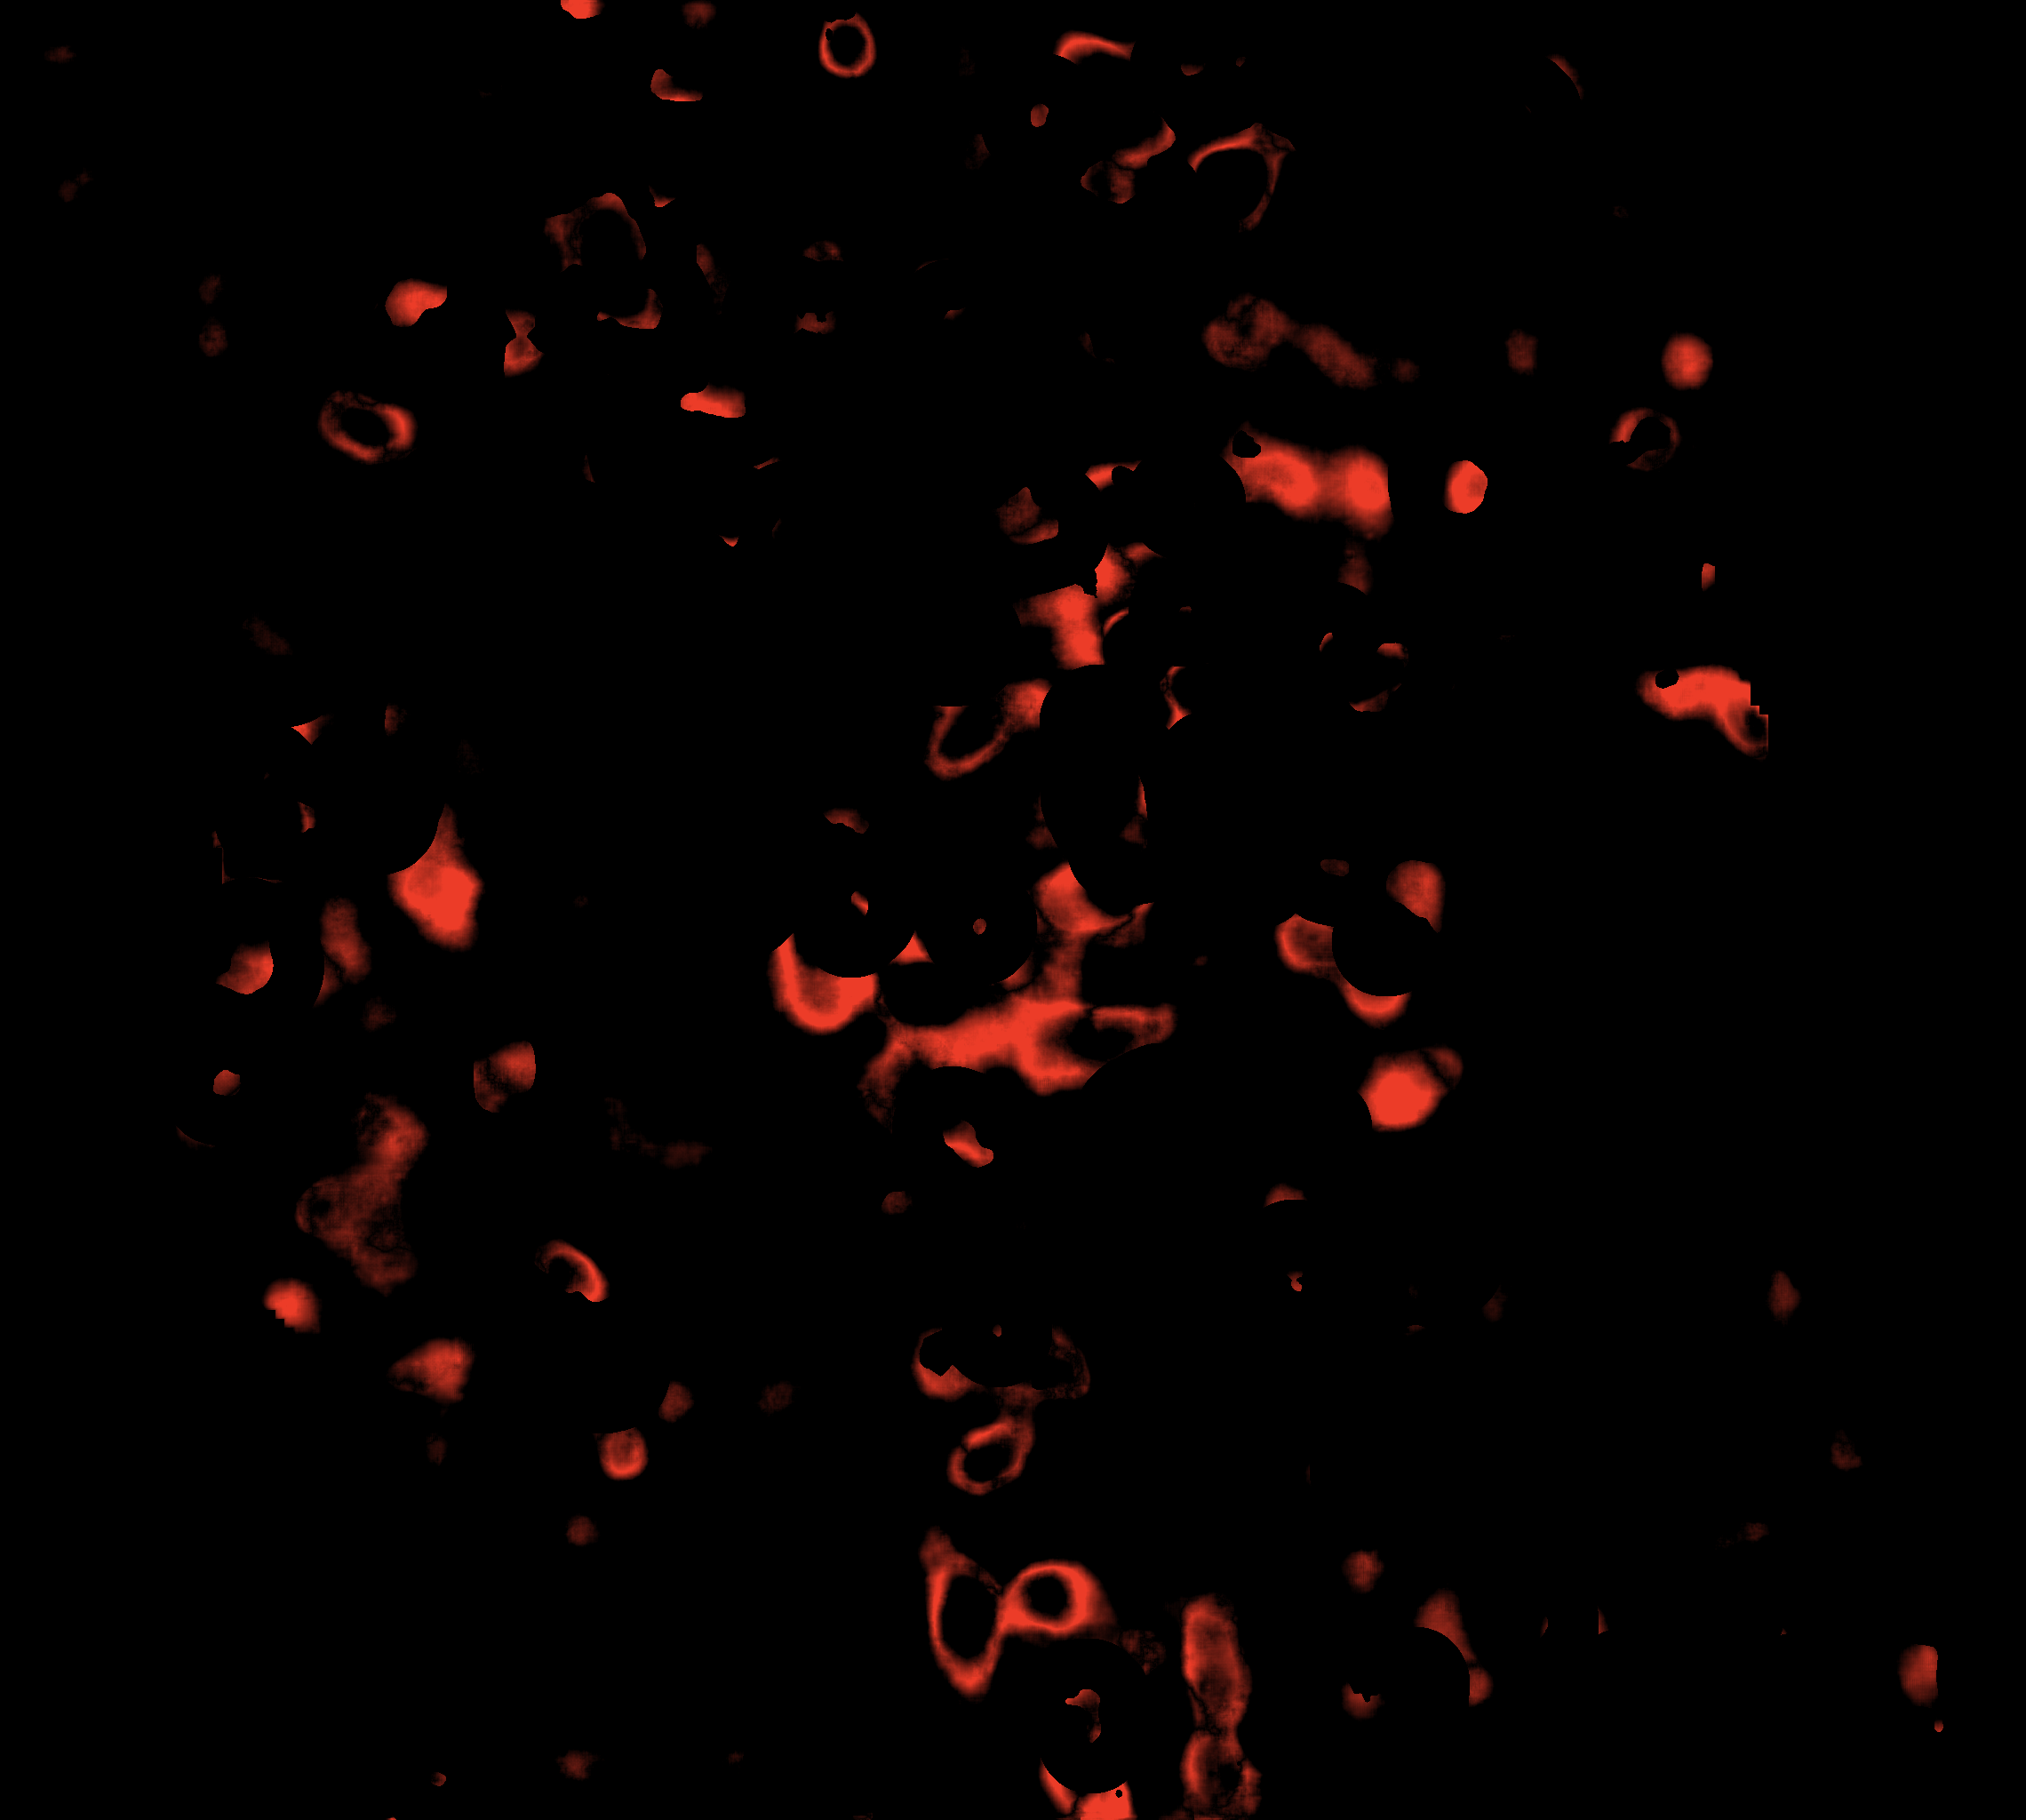
\includegraphics[width=0.29\textwidth]{../figures/m3/20250905172054-1_b2_3_difference.png}
\caption{Held-out unit 0343P$\cdot$172054-1. Left, Reader v3 (AUC 0.7573); centre, \MtName{} (AUC 0.7838); right, the red difference between the two maps. Each map is stretched between its own percentiles, the panels are shown at the full resolution of the file.}\label{fig:m3-20250905172054-1b2}
\end{figure*}
